% This is the Reed College LaTeX thesis template. Most of the work
% for the document class was done by Sam Noble (SN), as well as this
% template. Later comments etc. by Ben Salzberg (BTS). Additional
% restructuring and APA support by Jess Youngberg (JY).
% Your comments and suggestions are more than welcome; please email
% them to cus@reed.edu
%
% See http://web.reed.edu/cis/help/latex.html for help. There are a
% great bunch of help pages there, with notes on
% getting started, bibtex, etc. Go there and read it if you're not
% already familiar with LaTeX.
%
% Any line that starts with a percent symbol is a comment.
% They won't show up in the document, and are useful for notes
% to yourself and explaining commands.
% Commenting also removes a line from the document;
% very handy for troubleshooting problems. -BTS

% As far as I know, this follows the requirements laid out in
% the 2002-2003 Senior Handbook. Ask a librarian to check the
% document before binding. -SN

%%
%% Preamble
%%
% \documentclass{<something>} must begin each LaTeX document
\documentclass[12pt,twoside]{ugathesis}
% Packages are extensions to the basic LaTeX functions. Whatever you
% want to typeset, there is probably a package out there for it.
% Chemistry (chemtex), screenplays, you name it.
% Check out CTAN to see: http://www.ctan.org/
%%
\usepackage{graphicx,latexsym}
\usepackage[french]{babel}
\usepackage{amsmath}
\usepackage{amssymb,amsthm}
\usepackage[dvipsnames]{xcolor} % tk: for more color
\usepackage{xcolor}
\usepackage{eso-pic}
\usepackage{longtable,booktabs,setspace}
\usepackage{chemarr} %% Useful for one reaction arrow, useless if you're not a chem major
\usepackage[hyphens]{url}
\usepackage{pdfpages}
\usepackage{tikz}
\usetikzlibrary{calc}
% Added by CII
\usepackage{hyperref}
\usepackage{lmodern}
\usepackage{float}
\floatplacement{figure}{H}
% End of CII addition
\usepackage{rotating}
\usepackage{upgreek} % tk : pour pouvoir utiliser le symbole µ droit (pas en itallic)
\usepackage{pdfpages} % tk : pour pouvoir insérer des fichiers pdf dans le corp de texte
\usepackage{lscape} % tk : pour pouvoir insérer des images au format paysage
\newcommand{\blandscape}{\begin{landscape}}
\newcommand{\elandscape}{\end{landscape}}
\usepackage[utf8]{inputenc}

% Next line commented out by CII
%%% \usepackage{natbib}
% Comment out the natbib line above and uncomment the following two lines to use the new
% biblatex-chicago style, for Chicago A. Also make some changes at the end where the
% bibliography is included.
%\usepackage{biblatex-chicago}
%\bibliography{thesis}


% Added by CII (Thanks, Hadley!)
% Use ref for internal links
\renewcommand{\hyperref}[2][???]{\autoref{#1}}
\def\chapterautorefname{Chapter}
\def\sectionautorefname{Section}
\def\subsectionautorefname{Subsection}
% End of CII addition

% Added by CII
\usepackage{caption}
\captionsetup{width=5in}
% End of CII addition

% \usepackage{times} % other fonts are available like times, bookman, charter, palatino


% To pass between YAML and LaTeX the dollar signs are added by CII
\title{THÈSE}
\author{Thomas Karaouzene}
\lab{Génétique, Epigénétique et Thérapies de l'Infertilité (GETI) et
Techniques de l'Ingénierie Médicale et de la Complexité - Informatique,
Mathématiques et Applications de Grenoble (TIMC-IMAG)}
\date{07 novembre 2017}
\division{Mathematics and Natural Sciences}
\advisor{Pierre Ray}
%If you have two advisors for some reason, you can use the following
% Uncommented out by CII
\altadvisor{Nicolas Thierry-Mieg}
% End of CII addition
%\institution{}
%\degree{}

%%% Remember to use the correct department!
\department{Ingénierie de la Santé, de la Cognition et Environnement (EDISCE)}
% if you're writing a thesis in an interdisciplinary major,
% uncomment the line below and change the text as appropriate.
% check the Senior Handbook if unsure.
%\thedivisionof{The Established Interdisciplinary Committee for}
% if you want the approval page to say "Approved for the Committee",
% uncomment the next line
%\approvedforthe{Committee}

% Added by CII
%%% Copied from knitr
%% maxwidth is the original width if it's less than linewidth
%% otherwise use linewidth (to make sure the graphics do not exceed the margin)
\makeatletter
\def\maxwidth{ %
  \ifdim\Gin@nat@width>\linewidth
    \linewidth
  \else
    \Gin@nat@width
  \fi
}
\makeatother

\renewcommand{\contentsname}{Table of Contents}
% End of CII addition

\setlength{\parskip}{0pt}

% Added by CII
  %\setlength{\parskip}{\baselineskip}
  \usepackage[parfill]{parskip}

\providecommand{\tightlist}{%
  \setlength{\itemsep}{0pt}\setlength{\parskip}{0pt}}

\Acknowledgements{

}

\Dedication{

}

\Preface{

}

\Abstract{

}

	\usepackage{tikz}
% End of CII addition
%%
%% End Preamble
%%
%

\usepackage{amsthm}
\newtheorem{theorem}{Theorem}[chapter]
\newtheorem{lemma}{Lemma}[chapter]
\theoremstyle{definition}
\newtheorem{definition}{Definition}[chapter]
\newtheorem{corollary}{Corollary}[chapter]
\newtheorem{proposition}{Proposition}[chapter]
\theoremstyle{definition}
\newtheorem{example}{Example}[chapter]
\theoremstyle{definition}
\newtheorem{exercise}{Exercise}[chapter]
\theoremstyle{remark}
\newtheorem*{remark}{Remark}
\newtheorem*{solution}{Solution}
\begin{document}

% Everything below added by CII
  \maketitle

\frontmatter % this stuff will be roman-numbered
\pagestyle{empty} % this removes page numbers from the frontmatter



  \hypersetup{linkcolor=black}
  \setcounter{tocdepth}{3}
  \tableofcontents

  \listoftables

  \listoffigures



\mainmatter % here the regular arabic numbering starts
\pagestyle{fancyplain} % turns page numbering back on

\chapter*{Remerciements}\label{remerciements}
\addcontentsline{toc}{chapter}{Remerciements}

Je remercie Messieurs le \ldots{} et le \ldots{} d'avoir accepté la
charge d'être rapporteurs de ma thèse.

Je remercie Messieurs \ldots{} et \ldots{} d'avoir accepté de participer
à mon jury et juger ce travail.

À Agnès et Gérard pour avoir pris le temps de relir mon manuscrit et
corrigé mes nombreuses fautes.

À mes amis, toujours présents malgré la distance.

À l'ensemble du Budo club de Malesherbes et plus particulièrement à
Maître Hiram et Fanfan, qui m'ont vu grandir et qui, à travers leurs
enseignements du Karaté, ont réussi à me transmettre des valeurs et un
code de vie.

À ma famille pour son union et sa solidarité.

À Dadette et Marco pour m'avoir acqueilli pendant ces cinq années, et
tout les débats parfois endiablés que nous avons pu avoir ensemble.
``\emph{Hakuna matata}''.

À Aurélien pour tous ces moments de ``luronage'', les grecs, les parties
de tarots, nos années \emph{Bell \& Barksdale}. N'oublie jamais,
``\emph{le lion ne pactise pas avec les hommes}''.

À mes parents, pour avoir toujours été à mes côtés quelques soit mes
choix. Pour votre amour et votre devouement indéfectible. Votre mission
est desormai accomplie, profitez bien de votre vie de grands-parents.

À ma soeur pour toutes ces années de complicité. Bonne chance dans ta
nouvelle vie qui commence.

À Estelle, mon garde fou. Tu as su pendant ces années me conseiller et
me soutenir sans jamais faillir. Tu as toujours été là pour moi. Ta
capacité à me supporter est la preuve de ton courrage et ta force. Tu
m'as donné le plus beau des cadeaux en me permettant de construire, avec
toi, une famille. Tu es la clef de voute sur laquelle je me repose (trop
souvent). J'espère sincèrement que ces dix années ne sont que les
prémisses de notre Histoire et sache que tu pourras toujours compter sur
moi comme je compte sur toi.

À Noham, mon fils, ma plus grande fierté et source de bonheur. Tu as
boulversé ma vie . Ton seul rire à le pouvoir de me rendre heureux et de
me faire oublier tous mes tracas. Puisses-tu mener ta vie comme tu
l'entends, faire tes propres choix, tes propres erreurs en sachant que
je te soutiendrai toujours. Je t'aime.

\chapter*{Résumé}\label{resume}
\addcontentsline{toc}{chapter}{Résumé}

\newpage

Ces dix dernières années, l'investigation des maladies génétiques a été
bouleversée par l'émergence des techniques de séquençage haut-débit.
Celles-ci permettent désormais de ne plus séquencer les gènes un par un,
mais d'avoir accès à l'intégralité de la séquence génomique ou
transcriptomique d'un individu. La difficulté devient alors d'identifier
les variants causaux parmi une multitude d'artefacts techniques et de
variants bénins, pour ensuite comprendre la physiopathologie des gènes
identifiés.

L'application du séquençage haut débit est particulièrement prometteuse
dans le champ de la génétique de l'infertilité masculine car il s'agit
d'une pathologie dont l'étiologie est souvent génétique, qui est
génétiquement très hétérogène et pour laquelle peu de gènes ont été
identifiés. Mon travail de thèse est donc centré sur la l'infertilité et
comporte deux parties majeures : l'analyse des données issues du
séquençage haut débit d'homme infertiles et de modèles animaux et la
caractérisation moléculaire d'un phénotype spécifique d'infertilité, la
globozoospermie.

Le nombre de variants identifiés dans le cadre d'un séquençage exomique
pouvant s'élever à plusieurs dizaines de milliers, l'utilisation d'un
outil informatique performant est indispensable. Pour arriver à une
liste de variants suffisamment restreinte pour pouvoir être interprétée,
plusieurs traitements sont nécessaires. Ainsi, j'ai développé un
pipeline d'analyse de données issues de séquençage haut-débit effectuant
de manière successive l'intégralité des étapes de l'analyse
bio-informatique, c'est-à-dire l'alignement des \emph{reads} sur un
génome de référence, l'appel des génotypes, l'annotation des variants
obtenus ainsi que le filtrage de ceux considérés comme non pertinents
dans le contexte de l'analyse. L'ensemble de ces étapes étant
interdépendantes, les réaliser au sein du même pipeline permet de mieux
les calibrer pour ainsi réduire le nombre d'erreurs générées. Ce
pipeline a été utilisé dans cinq études au sein du laboratoire, et a
permis l'identification de variants impactants des gènes candidats
prometteurs pouvant expliquer le phénotype d'infertilité des patients.
L'ensemble des variants retenus ont ensuite pu être validés
expérimentalement.

J'ai également pris part aux investigations génétiques et moléculaires
permettant la caractérisation du gène \emph{DPY19L2}, identifié au
laboratoire et dont la délétion homozygote entraine une globozoospermie,
caractérisée par la présence dans l'éjaculât de spermatozoïdes à tête
ronde dépourvus d'acrosome. Pour cela, j'ai contribué à caractériser les
mécanismes responsables de cette délétion récurrente, puis, en utilisant
le modèle murin \emph{Dpy19l2 knock out} (KO) mimant le phénotype
humain, j'ai réalisé une étude comparative des transcriptomes
testiculaires de souris sauvages et de souris KO
\emph{Dpy19l2\textsuperscript{-/-}}. Cette étude a ainsi permis de
mettre en évidence la dérégulation de 76 gènes chez la souris KO. Parmi
ceux-ci, 23 sont impliqués dans la liaison d'acides nucléiques et de
protéines, pouvant ainsi expliquer les défauts d'ancrage de l'acrosome
au noyau chez les spermatozoïdes globozoocéphales.

Mon travail a donc permis de mieux comprendre la globozoospermie et de
développer un pipeline d'analyse bioinformatique qui a déjà permis
l'identification de plus de 15 gènes de la gamétogénèse humaine
impliqués dans différents phénotypes d'infertilité.

\newpage

\chapter*{Abstract}\label{abstract}
\addcontentsline{toc}{chapter}{Abstract}

\newpage

In the last decade, the investigations of genetic diseases have been
revolutionized by the rise of high throughput sequencing (HTS). Thanks
to these new techniques it is now possible to analyze the totality of
the coding sequences of an individual (exome sequencing) or even the
sequences of his entire genome or transcriptome. The understanding of a
pathology and of the genes associated with it now depends on our ability
to identify causal variants within a plethora of technical artifact and
benign variants.

HTS is expected to be particularly useful in the field infertility as
this pathology is expected to be highly genetically heterogeneous and
only a few genes have so far been associated with it. My thesis focuses
on male infertility and is divided into two main parts: HTS data
analysis of infertile men and the molecular characterization of a
specific phenotype, globozoospermia.

Several thousands of distinct variants can be identified in a single
exome, thereby using effective informatics is essential in order to
obtain a short and actionable list of variants. It is for this purpose
that I developed a HTS data analysis pipeline performing successively
all bioinformatics analysis steps: 1) reads mapping along a reference
genome, 2) genotype calling, 3) variant annotation and 4) the filtering
of the variants considered as non-relevant for the analysis. Performing
all these independent steps within a single pipeline is a good way to
calibrate them and therefore to reduce the number of erroneous calls.
This pipeline has been used in five studies and allowed the
identification of variants impacting candidate genes that may explain
the patients' infertility phenotype. All these variants have been
experimentally validated using Sanger sequencing.

I also took part in the genetic and molecular investigations which
permitted to demonstrate that the absence of the \emph{DPY192} gene
induces male infertility due to globozoospermia, the presence in the
ejaculate of only round-headed and acrosomeless spermatozoa. Most
patients with globozoospermia have a homozygous deletion of the whole
gene. I contributed to the characterization of the mechanisms
responsible for this recurrent deletion, then, using \emph{Dpy19l2}
knockout (KO) mice, I realized the comparative study of testicular
transcriptome of wild type and \emph{Dpy19l2}\textsuperscript{-/-} KO
mice. This study highlighted a dysregulation of 76 genes in KO mice.
Among them, 23 are involved in nucleic acid and protein binding, which
may explain acrosome anchoring defaults observed in the sperm of
globozoospermic patients.

My work allowed a better understanding of globozoospermia and the
development of a HTS data analysis pipeline. The latter allowed the
identification of more than 15 human gametogenesis genes involved in
different infertility phenotypes.

\chapter{Introduction}\label{introInf}

\section{La spermatogenèse}\label{la-spermatogenese}

La spermatogenèse des mammifères est un processus long et complexe
contrôlé par plusieurs mécanismes étroitement liés
{[}\protect\hyperlink{ref-Gnessi1997}{1}--\protect\hyperlink{ref-KIERSZENBAUM1994}{3}{]}.
C'est au cours de celle-ci, qu'à partir de cellules germinales, seront
produits les spermatozoïdes matures. Ce processus est divisé en trois
phases principales : la phase de multiplication, la phase de division
(appelée la \protect\hyperlink{meiose}{méiose}) et la phase de
maturation. Chez les hommes, ces étapes se déroulent en continu dans la
paroi des tubes séminifères du testicule depuis la puberté jusqu'à la
mort et impliquent trois types de cellules germinales : les
spermatogonies, les spermatocytes et les spermatides. Le temps
nécessaire pour obtenir un spermatozoïde mature à partir de cellules
germinales est de 74 jours et la production quotidienne de
spermatozoïdes s'élève environ à 45 millions par testicule
{[}\protect\hyperlink{ref-Johnson1980}{4}{]}. Le cycle spermatogénétique
est défini comme la succession chronologique des différents stades de
différenciation d'une génération de cellules germinales (depuis la
spermatogonie jusqu'au spermatozoïde). Chacune des étapes du cycle
spermatogénétique a une durée fixe et constante selon les espèces
(\textbf{Table : }\ref{tab:spermatotime}).

\begin{longtable}[t]{ll}
\caption{\label{tab:spermatotime}Durée de vie moyenne des cellules germinales humaines}\\
\toprule
Cellules germinales & Durée de vie moyenne (jours)\\
\midrule
Spermatogonies Ap & 16-18\\
Spermatogonie B & 7.5-9\\
Spermatocytes primaires & 23\\
Spermatocytes secondaires & 1\\
Spermatides & 1\\
\bottomrule
\end{longtable}

\newpage

\subsection{Rappels sur le testicule}\label{rappels-sur-le-testicule}

Les testicules sont les organes sexuels masculins. Ils possèdent deux
fonctions principales plus ou moins exprimées selon les périodes de la
vie de l'individu : une fonction endocrine caractérisée par la synthèse
des hormones stéroïdes sexuelles masculines (la stéroïdogenèse) et une
fonction exocrine au cours de laquelle seront produits les gamètes
masculins. Chez un individu adulte en bonne santé, le testicule présente
une forme ovoïde ayant un volume moyen de 18 cm\textsuperscript{3}. Chez
l'homme, comme chez la plupart des mammifères terrestres, ils sont
localisés sous le pénis dans une poche de peau appelée scrotum et reliés
à l'abdomen par le cordon spermatique (\textbf{Figure :}
\ref{fig:testicule}). Cette externalisation des testicules permet leur
maintien à une température plus basse que celle du reste du corps,
nécessaire à la spermatogenèse.

L'intérieur du testicule contient des tubes séminifères enroulés ainsi
que du tissu entre les tubules appelé espace interstitiel. Les tubes
séminifères sont de longs tubes compactés sous forme de boucles et dont
les deux extrémités débouchent sur le \emph{rete testis} (\textbf{Figure
:} \ref{fig:testicule}). C'est le long des parois du tube séminifère que
se déroulera l'ensemble des étapes de la spermatogenèse.

\begin{figure}

{\centering 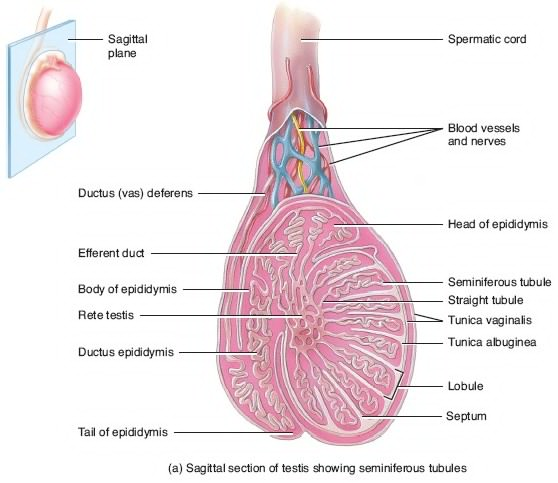
\includegraphics[scale=0.65]{figure/coupe_testicule2} 

}

\caption[Schéma anatomique du testicule humain]{\textbf{\emph{Schéma anatomique du testicule humain}.}}\label{fig:testicule}
\end{figure}



\newpage

\subsection{La phase de
multiplication}\label{la-phase-de-multiplication}

La phase de multiplication est la phase au cours de laquelle les
spermatogonies se divisent par mitoses pour aboutir au stade de
spermatocytes primaires. Les spermatogonies sont des cellules diploïdes
à l'origine de l'ensemble des autres cellules germinales humaines. Pour
cela, elles vont s'auto-renouveler par mitoses successives afin de
maintenir une production continue de spermatozoïdes tout au long de la
vie de l'individu. Ces cellules sont localisées dans le compartiment
basal des tubes séminifères. Les analyses histologiques ont permis de
distinguer trois types de spermatogonies en fonction de leur contenu en
hétérochromatine
{[}\protect\hyperlink{ref-Clermont1963}{5}--\protect\hyperlink{ref-Goossens2013}{7}{]}
: Les spermatogonies de type A dark (ou Ad), les spermatogonies de type
A pale (ou Ap) et les spermatogonies de type B.

Chez l'Homme, les spermatogonies Ad ont une activité mitotique au cours
de la spermatogénèse et servent de réserve. Elles vont au cours d'une
première mitose former une spermatogonie Ad et un spermatogonie Ap
(\textbf{Figure :} \ref{fig:spermatogenese}). Cette propriété permet à
la fois de se différencier en spermatocytes tout en constituant un
compartiment de réserve de spermatogonies Ad pour la régénération de la
population de cellules germinales au sein de l'épithélium séminifère.
L'entrée en division des spermatogonies Ap se fait par groupes
cellulaires tous les 16 jours. Les cellules d'une même génération
maintiennent entre elles des ponts cytoplasmiques jusqu'à la
\protect\hyperlink{spermiogenese}{spermiogenèse} ce qui permet la
synchronisation parfaite du développement gamétique de toutes les
cellules filles issues d'un groupe de spermatogonies Ap. Ce phénomène
est appelé onde spermatogénétique. Chaque spermatogonie Ap va former,
lorsqu'elle se divise par mitose, deux spermatogonies B qui elles-mêmes
se diviseront en deux spermatocytes primaires diploïdes (\textbf{Figure
:} \ref{fig:spermatogenese}).

\newpage

\begin{figure}

{\centering 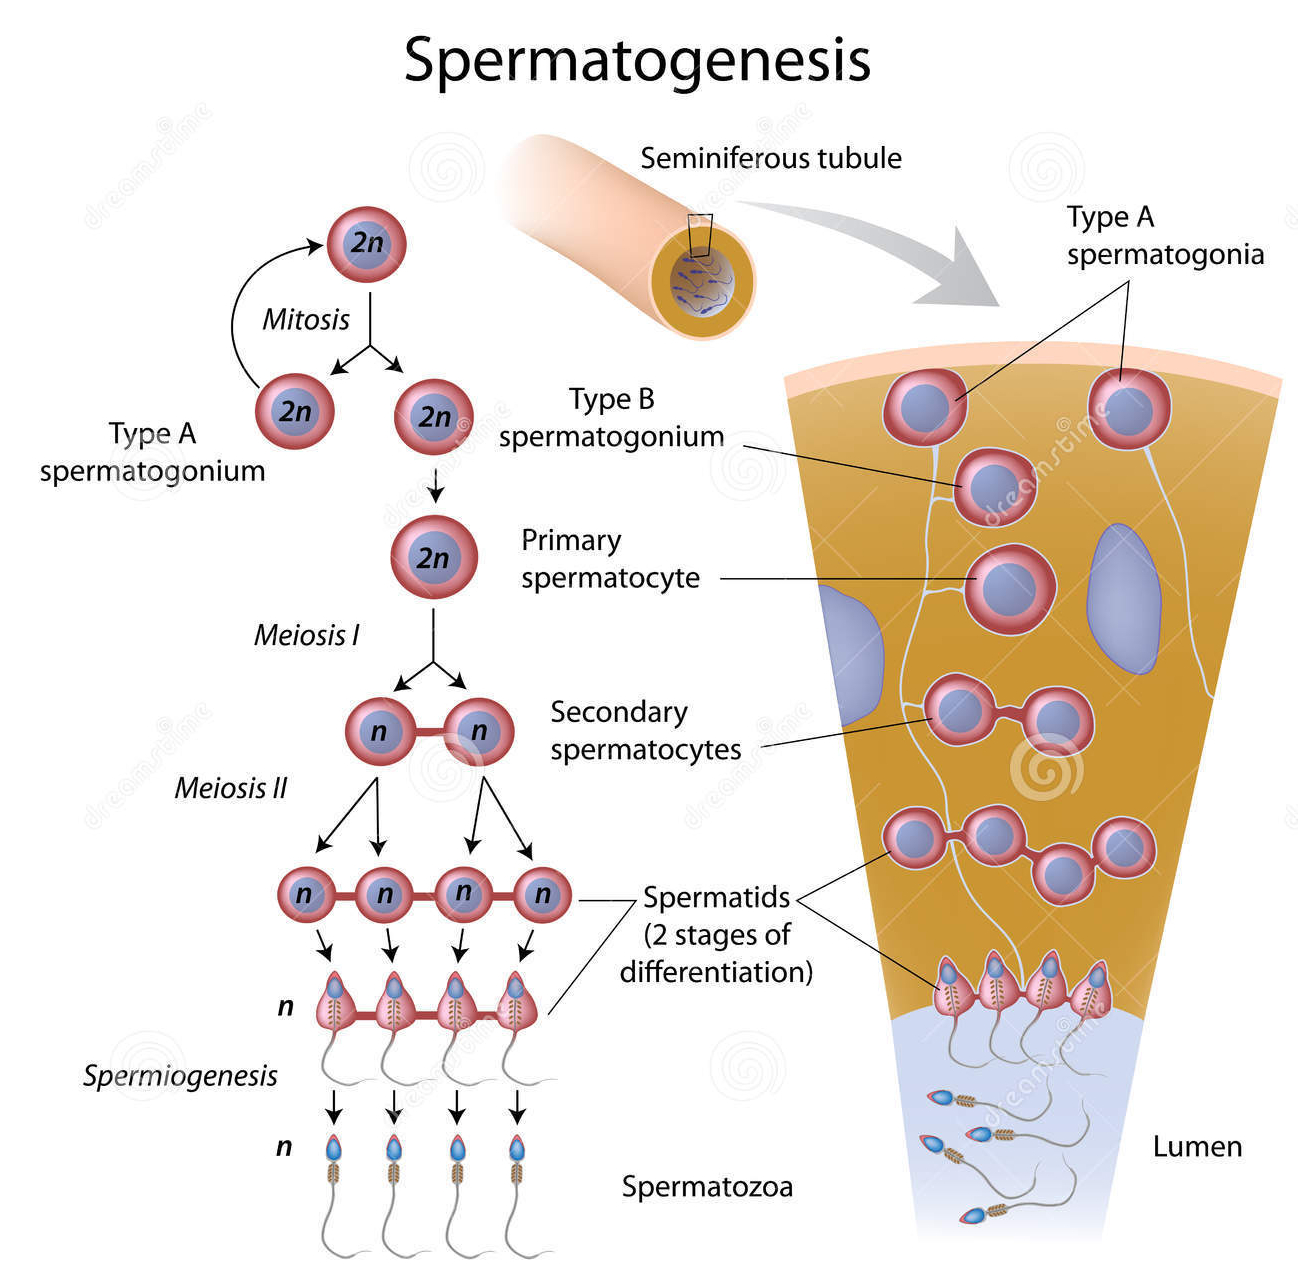
\includegraphics[scale=0.35]{figure/spermatogenese2} 

}

\caption[Les différentes phases de la spermatogenèse]{\textbf{\emph{Les différentes phases de la
spermatogenèse} d'après
\href{http://www.medizin-kompakt.de/spermatogenese}{medizin-kompakt}} :
L'évolution de la spermatogenèse est strictement coordonnée, tant dans
le sens transversal des tubules, que dans le sens longitudinal. Le sens
transversal correspond au sens unique de la différenciation germinale,
les cellules souches sont situées à la base du tube séminifère alors que
les spermatozoïdes aboutissent à la lumière. Dans le sens longitudinal
de ces tubules, on retrouve l'ensemble des cellules d'un même cycle
donnant ainsi l'onde spermatique.}\label{fig:spermatogenese}
\end{figure}












\newpage 

\hypertarget{meiose}{\subsection{La méiose}\label{meiose}}

La méiose, ou phase de maturation, est l'étape au cours de laquelle, à
partir de cellules diploïdes (les spermatogonies B) vont se former des
cellules haploïdes, les spermatocytes secondaires (spermatocytes II). Ce
résultat est le fruit de deux divisions successives (\textbf{Figure :
}\ref{fig:pictmeiose}) appelées respectivement méiose réductionnelle ou
méiose I (MI) et méiose équationnelle ou méiose II (MII). La MI va
séparer les chromosomes homologues, produisant deux cellules et
réduisant la ploïdie de diploïde à haploïde (d'où son nom
\emph{réductionnelle}). En plus de son rôle de division vu précédemment,
la méiose joue un rôle clef dans le brassage génétique (mélange des
gènes) et ce, grâce à deux mécanismes de brassage : le brassage
inter-chromosomique, lorsque les chromosomes sont séparés et le brassage
intra-chromosomique impliquant notamment des enjambements chromosomiques
(crossing-over) (\textbf{Figure : }\ref{fig:pictcrossingover}).

La méiose est initiée dès la fin de la phase de multiplication à partir
des spermatocytes primaires issus de la division des spermatogonies de
type B. Ces cellules nouvellement formées se situent dans le
compartiment basal du tube séminifère. C'est là qu'elles vont tout
d'abord subir une interphase (stade préleptotène) durant entre 2 et 4
jours. Au cours de cette phase a lieu la réplication de l'ADN. Cette
réplication se fait lorsque l'ADN est à l'état de chromatine, pendant la
phase S (pour synthèse) de l'interphase. À l'issue de cette phase,
chaque chromosome sera composé de deux chromatides reliées entre elles
par le centromère, le matériel génétique de chaque cellule ayant donc
été multiplié par deux. Par la suite, ces cellules vont subir deux
divisions méiotiques, chacune composée de quatre étapes distinctes
(\textbf{Figure : }\ref{fig:pictmeiose}) :

\begin{figure}

{\centering 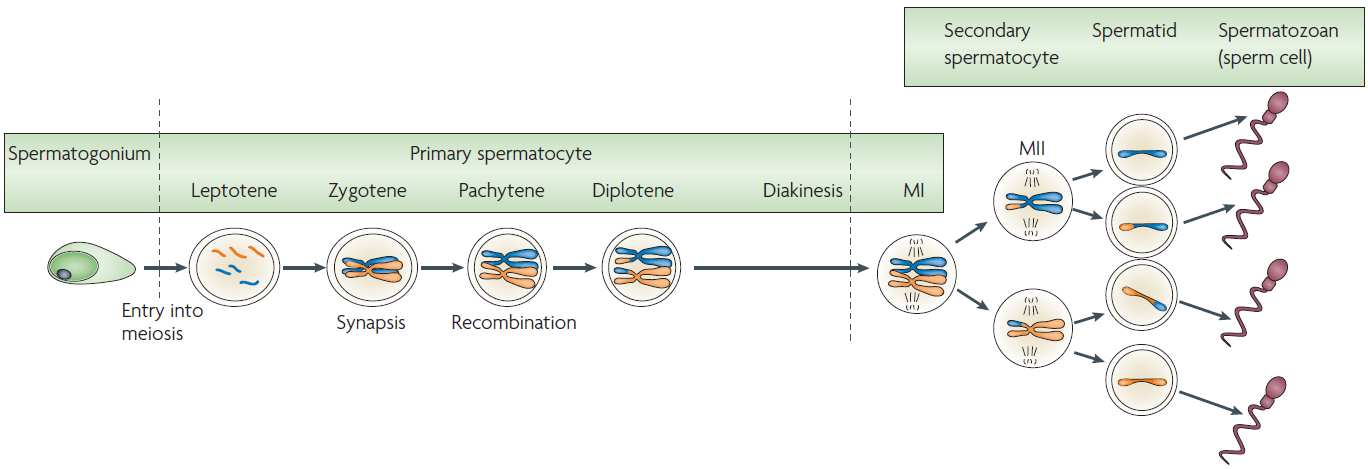
\includegraphics[scale=0.33]{figure/Meiosis_Stages} 

}

\caption[Les différentes étapes de la méiose gamétique masculine]{\textbf{\emph{Les différentes étapes de la méiose
gamétique masculine} d'après
{[}\protect\hyperlink{ref-Sasaki2008}{8}{]}} : Les spermatogonies B
servent de point d'initiation et se différentient en spermatocyte
primaire. Les cinq étapes de la prophase I sont suivient d'une première
division cellulaire, donnant deux cellules haploides au sein desquelles
les chromosomes sont composés de deux chromatides. Celles-ci seront
séparées au cours de la méiose II donnant ainsi quatre spermatides qui
après plusieurs étapes de maturation donneront les spermatozoïdes.}\label{fig:pictmeiose}
\end{figure}











\newpage

\begin{enumerate}
\def\labelenumi{\arabic{enumi}.}
\tightlist
\item
  \textbf{Méiose réductionnelle} : (\textbf{Figure : }\ref{fig:meiosei})

  \begin{enumerate}
  \def\labelenumii{\alph{enumii}.}
  \item
    \textbf{La prophase I} : cette longue étape dure 23 jours chez
    l'homme et peut être subdivisée en cinq phases successives :
    leptotène, zygotène, pachytène, diplotène et diacinèse.

    \begin{enumerate}
    \def\labelenumiii{\roman{enumiii}.}
    \tightlist
    \item
      \textbf{Leptotène} : condensation de la chromatine et formation
      des chromosomes.\\
    \item
      \textbf{Zygotène} : appariement des chromosomes homologues par
      paires appelés bivalents grâce à l'intermédiaire d'une structure
      multi-protéique : le complexe synaptonémal.\\
    \item
      \textbf{Pachytène} : ce stade dure 16 jours. Il est le plus long
      de la prophase I. C'est au cours de celui-ci, qu'a lieu l'échange
      de matériel génétique par le biais des crossing-over entre les
      chromatides non-sœurs appelées nodules de recombinaison
      (\textbf{Figure : }\ref{fig:pictcrossingover}).\\
    \item
      \textbf{Diplotène} : la dissociation du complexe synaptonémal va
      permettre aux chromosomes homologues d'initier leur séparation.
      Certains sites d'appariement étroits nommés chiasmas demeurent
      néanmoins liés permettant une séparation plus progressive des
      chromosomes et réduisant ainsi le risque d'aneuploïdies (nombre
      anormal de chromosomes)
      {[}\protect\hyperlink{ref-Handyside2012}{9}{]}.\\
    \item
      \textbf{Diacinèse} : cette étape marque la fin de la méiose I et
      fait office de transition avec la méiose II. Elle est caractérisée
      par une condensation maximale des chromosomes et la disparition de
      la membrane nucléaire et du nucléole. Le fuseau méiotique commence
      à s'assembler, les centromères des chromosomes homologues
      s'éloignent et les chiasmas glissent progressivement vers les
      télomères.\\
    \end{enumerate}
  \item
    \textbf{La métaphase I} : phase au cours de laquelle les chromosomes
    vont s'aligner à l'équateur de la cellule pour former la plaque
    équatoriale.
  \item
    \textbf{L'anaphase I} : les chromatides sœurs (ou les chromosomes
    homologues en fonction de la phase méiotique) vont se séparer et
    migrer aux pôles opposés de la cellule.\\
  \item
    \textbf{La télophase I} : qui est l'étape finale, les chromosomes se
    décondensent et l'enveloppe nucléaire se reforme autour des
    chromosomes. La cellule mère se sépare alors en deux cellules filles
    appelées spermatocytes secondaires.
  \end{enumerate}
\end{enumerate}

\newpage

\begin{enumerate}
\def\labelenumi{\arabic{enumi}.}
\setcounter{enumi}{1}
\tightlist
\item
  \textbf{Méiose équationnelle} : (\textbf{Figure : }\ref{fig:meioseii})
  la MII est similaire à une division mitotique et peut se décomposer en
  quatre parties distinctes :

  \begin{enumerate}
  \def\labelenumii{\alph{enumii}.}
  \tightlist
  \item
    \textbf{La prophase II} : contrairement à la prophase I, la prophase
    II est très courte. Les chromosomes alors formés de deux chromatides
    sœurs se dirigent vers la plaque équatoriale.\\
  \item
    \textbf{La métaphase II} : à ce stade, les chromosomes sont alignés
    le long de la plaque équatoriale au niveau de leur centromère.\\
  \item
    \textbf{L'anaphase II} : les centromères de chaque chromosome se
    séparent permettant aux chromatides sœurs de se diriger vers les
    pôles opposés des spermatocytes II.\\
  \item
    \textbf{La télophase II} : comme en télophase I, les cellules mères
    se séparent en deux cellules filles haploïdes appelées spermatides,
    contenant chacune n chromosomes.
  \end{enumerate}
\end{enumerate}

\begin{figure}

{\centering 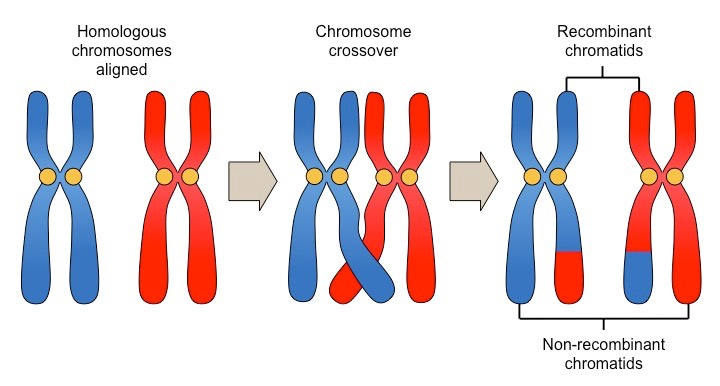
\includegraphics[scale=0.35]{figure/crossingover} 

}

\caption[Schéma simplifié d'un enjambement chromosomique (crossing-over)]{\textbf{\emph{Schéma simplifié d'un enjambement
chromosomique (crossing-over)}.}}\label{fig:pictcrossingover}
\end{figure}




\newpage 

\begin{figure}

{\centering 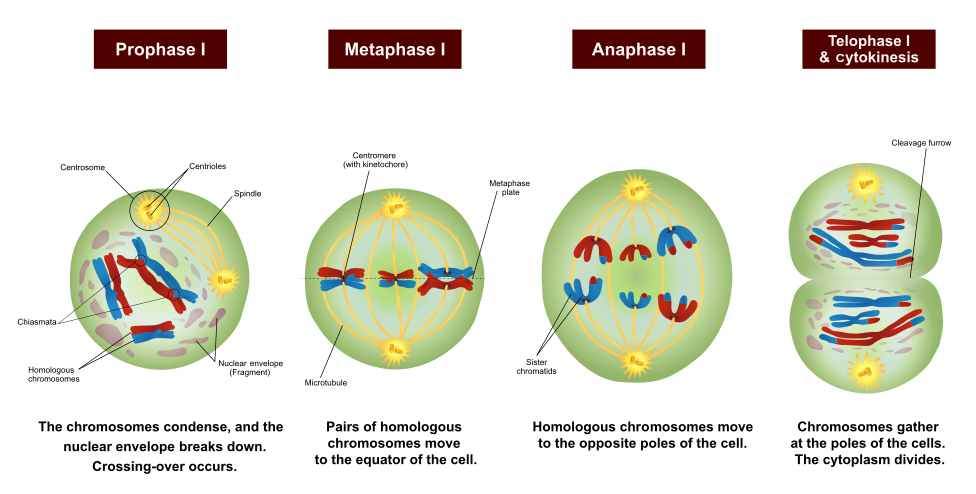
\includegraphics[scale=0.43]{figure/MeiosisI} 

}

\caption[Les différentes étapes de la première division méiotique masculine]{\textbf{\emph{Les différentes étapes de la première
division méiotique masculine} adapté
d'après{[}\protect\hyperlink{ref-Reece2014}{10}{]}}.}\label{fig:meiosei}
\end{figure}





\begin{figure}

{\centering 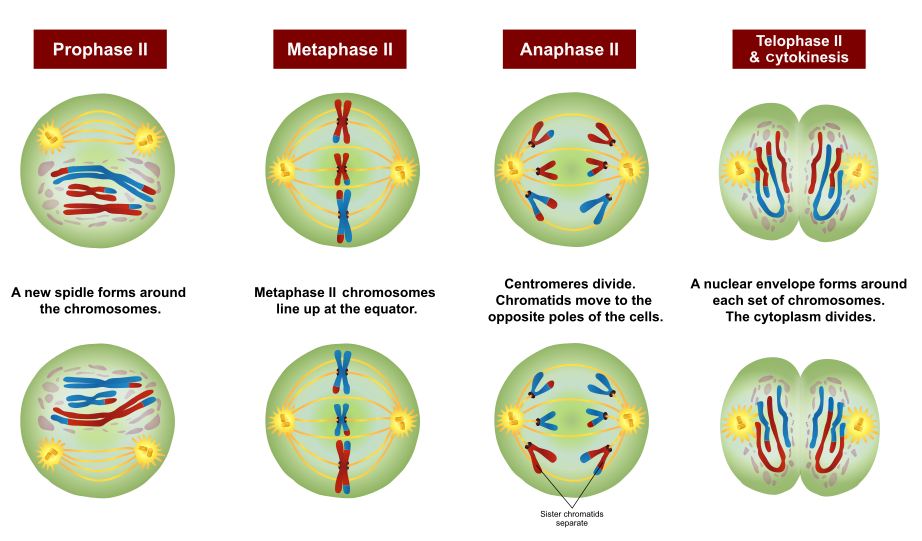
\includegraphics[scale=0.43]{figure/MeiosisII} 

}

\caption[Les différentes étapes de la deuxième division méiotique masculine]{\textbf{\emph{Les différentes étapes de la deuxième
division méiotique masculine} adapté
d'après{[}\protect\hyperlink{ref-Reece2014}{10}{]}}.}\label{fig:meioseii}
\end{figure}





\newpage

\hypertarget{spermiogenese}{\subsection{La
spermiogenèse}\label{spermiogenese}}

La spermiogenèse est la phase finale de la spermatogenèse. Elle dure
environ 23 jours chez l'humain et peut être subdivisée en sept étapes
(\textbf{Figure : }\ref{fig:spermiogenese}). La spermiogenèse définit la
cytodifférentiation des spermatides en spermatozoïdes. C'est au cours de
cette phase que les caractéristiques morphologiques et fonctionnelles du
spermatozoïde seront déterminées
{[}\protect\hyperlink{ref-YvesClermontRichardOko1993}{11}{]}. Elle est
caractérisée par trois évènements majeurs : la formation de l'acrosome,
la compaction de l'ADN nucléaire et la formation du flagelle. Le
développement de l'acrosome et la formation du flagelle commencent au
niveau des spermatides rondes
{[}\protect\hyperlink{ref-Escalier1991}{12}{]}. Pendant l'élongation de
la spermatide, le noyau se condense et devient hautement polarisé
{[}\protect\hyperlink{ref-Hamilton1987}{13}{]}. Les spermatides sont
situées dans le compartiment adluminal, à proximité de la lumière du
tube séminifère. Ce sont de petites cellules (8 à 10 \(\upmu\)m) que
l'on peut schématiquement diviser en trois classes :

\begin{enumerate}
\def\labelenumi{\arabic{enumi}.}
\item
  \textbf{Les spermatides rondes} (\textbf{Figure :
  }\ref{fig:spermiogenese} - \textbf{1} et \textbf{2}) :
  l'identification de ces cellules représente une difficulté technique.
  Elles ont cependant pu être décrites en détail par différentes
  techniques de coloration sous microscope optique
  {[}\protect\hyperlink{ref-Clermont1963}{5},
  \protect\hyperlink{ref-Papic}{14}--\protect\hyperlink{ref-WorldHealthOrganization1992}{17}{]}.
  Plusieurs études animales ont pu démontrer le potentiel des
  spermatides rondes à donner la vie à des individus sains et fertiles,
  {[}\protect\hyperlink{ref-Ogura1994}{18}--\protect\hyperlink{ref-Sasagawa}{20}{]},
  la même chose ayant été également observée plus récemment chez l'homme
  {[}\protect\hyperlink{ref-Tanaka2015}{21}{]} bien que le taux de
  fécondation et d'implantation soit extrêmement faible
  {[}\protect\hyperlink{ref-Asimakopoulos2003}{22}{]}. Ils possèdent un
  noyau rond avec une chromatine pâle et homogène. C'est à partir de ces
  étapes que démarre la biogenèse de l'acrosome avec la production par
  l'appareil de Golgi des vésicules pro-acrosomales (phase de Golgi).
  Les deux centrioles contenus dans le cytoplasme vont se déplacer au
  futur pôle caudal. Le centriole proximal est inactif alors que le
  centriole distal donne naissance à un ensemble de microtubules à
  l'origine de l'axonème du futur flagelle.
\item
  \textbf{Les spermatides en élongation} (\textbf{Figure :
  }\ref{fig:spermiogenese} - \textbf{3} et \textbf{4}) : à ce stade,
  l'acrosome va s'étendre le long du noyau lui donnant une forme plus
  allongée et la chromatine devient plus sombre. Un réseau de
  microtubules se forment autour du noyau créant ainsi la manchette qui
  participera également à l'allongement de la tête du spermatozoïde et
  permettra la migration des mitochondries vers la pièce intermédiaire
  du flagelle pour former le manchon de mitochondries
  {[}\protect\hyperlink{ref-Moreno2006}{23}{]}. Les spermatides en
  élongation peuvent aussi permettre la fécondation et d'initier des
  grossesses avec un meilleur taux de réussite que les spermatides
  rondes. De plus, ils engendreraient théoriquement moins de risques
  d'anomalies génétiques
  {[}\protect\hyperlink{ref-Asimakopoulos2003}{22}{]}.
\end{enumerate}

\newpage

\begin{enumerate}
\def\labelenumi{\arabic{enumi}.}
\setcounter{enumi}{2}
\tightlist
\item
  \textbf{Les spermatides en condensation} (\textbf{Figure :
  }\ref{fig:spermiogenese} - \textbf{5} et \textbf{7}) : c'est le stade
  final de la différenciation du spermatide en spermatozoïde. À ce stade
  le noyau est très allongé, avec une partie caudale globulaire et une
  partie antérieure saillante. La chromatine est sombre et condensée.
  L'axonème va continuer à s'allonger pour former le flagelle mature.
  Les différentes organelles inutiles pour la physiologique spermatique
  et l'excès de cytoplasme vont former la gouttelette cytoplasmique qui
  va se détacher et donner le corps résiduel qui va ensuite être
  phagocyté par les cellules de Sertoli
  {[}\protect\hyperlink{ref-Hermo2010}{24}{]}.
\end{enumerate}

Une fois ces étapes de différentiation finies, les spermatides sont
relâchées en tant que spermatozoïdes dans la lumière du tube séminifère.
Ce procédé est appelé spermiation.

\begin{figure}

{\centering 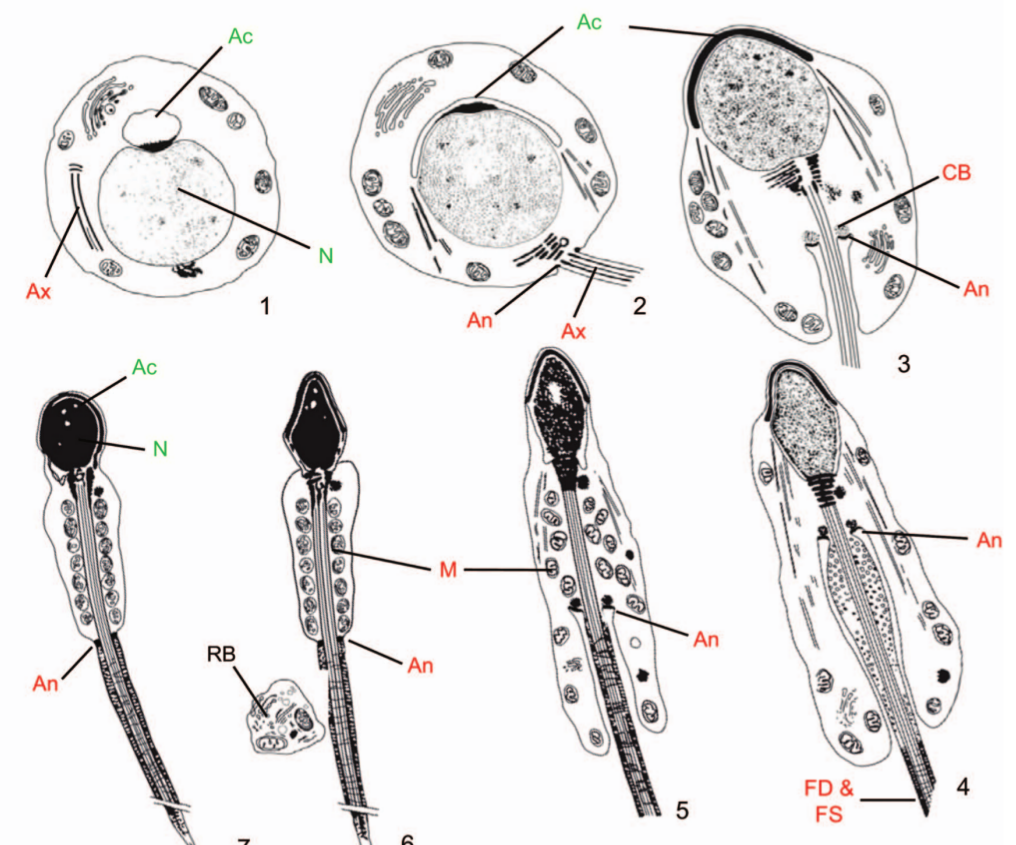
\includegraphics[scale=0.3]{figure/spermiogenese} 

}

\caption[Principales étapes et modifications structurales lors de la spermiogenèse]{\textbf{\emph{Principales étapes et modifications
structurales lors de la spermiogenèse}
d'après{[}\protect\hyperlink{ref-Toure2011}{25}{]}} : \textbf{1.} La
spermatide immature avec un gros noyau arrondi. La vésicule acrosomale
est attachée au noyau, l'ébauche du flagelle n'atteint pas le noyau.
\textbf{2.} La vésicule acrosomale a augmenté de taille et apparaît
aplatie au niveau du noyau. Le flagelle entre en contact avec le noyau.
\textbf{3-7.} Formation de l'acrosome, condensation du noyau et
développement des structures flagellaires. Ac = Acrosome, Ax = Axonème,
CC = Corps Chromatoïdes, CR = Corps Résiduel, FD = Fibres Denses, GF =
Gaine Fibreuse, M = Mitochondrie, Ma = Manchette.}\label{fig:spermiogenese}
\end{figure}













\newpage  

\section{Structure et fonction du
spermatozoïde}\label{structure-et-fonction-du-spermatozoide}

Le spermatozoïde est une cellule hautement différenciée dont la taille,
l'orientation et la symétrie sont déterminées. La morphologie générale
du spermatozoïde éjaculé est similaire à celle du spermatozoïde
testiculaire. Le spermatozoïde humain normal mature mesure environ 60
\(\upmu\)m de long et est essentiellement constitué de deux parties : la
tête et le flagelle (\textbf{Figure : }\ref{fig:spz}). En plus d'être
unique dans sa morphologie, le spermatozoïde l'est aussi dans sa
fonction puisque c'est la seule cellule produite de manière endogène et
dont l'action est exercée de manière exogène. La fécondation d'un
ovocyte par un spermatozoïde formera un zygote diploïde qui pourra se
développer ensuite en embryon dans l'uterus féminin.




\begin{figure}

{\centering 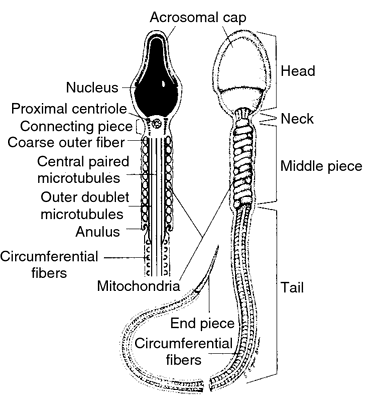
\includegraphics[scale=.75]{figure/sperm_anatomy} 

}

\caption[Anatomie simplifiée du spermatozoïde]{\textbf{\emph{Anatomie simplifiée du spermatozoïde} d'après
\href{http://medical-dictionary.thefreedictionary.com/Human+sperm}{medical-dictionary}}.}\label{fig:spz}
\end{figure}

\newpage

\subsection{La tête}\label{la-tete}

\begin{enumerate}
\def\labelenumi{\arabic{enumi}.}
\item
  \textbf{L'acrosome} : c'est une vésicule de sécrétion géante située
  dans la moitié supérieure de la tête du spermatozoïde. Elle se
  développe à partir de l'appareil de Golgi lors de la spermiogenèse. Au
  cours de sa formation, l'acrosome forme tout d'abord un granule
  sphérique qui se colle sur la partie apicale du noyau. En
  s'aplatissant contre celui-ci, l'acrosome va prendre une forme
  hémisphérique recouvrant la membrane nucléaire formant la coiffe
  céphalique. Le rôle de l'acrosome est fondamental dans le processus de
  fécondation puisqu'il permet d'excréter notamment l'acrosine, une
  enzyme de digestion permettant au spermatozoïde de traverser la zone
  pellucide qui entoure les ovocytes. Ce processus de relargage est
  appelé réaction acrosomale.
\item
  \textbf{L'acroplaxome} : l'acroplaxome est une structure cytosquelette
  composée de microfilaments d'actine (F- actine) et de kératine 5.
  Cette structure est positionnée en face de l'appareil de golgi et
  contre le noyau et sert de point d'attachement ainsi que de guide aux
  vésicules pro-acrosomales
  {[}\protect\hyperlink{ref-Kierszenbaum2004}{26}{]}. C'est une
  structure transitoire qui disparaît pour être remplacée par la thèque
  périnucléaire dans le spermatozoïde mature.
\item
  \textbf{Le noyau} : c'est une structure cellulaire présente dans la
  majorité des cellules eucaryotes. Il contient l'essentiel du matériel
  génétique. Le noyau du spermatozoïde est caractérisé par une
  compaction extrêmement importante de l'ADN. Dans les cellules
  somatiques l'ADN est enroulé par unité de 146 paires de bases autour
  d'un octamère d'histones dit de cœur (H2A, H2B, H3 et H4) afin
  d'organiser les trois milliards de paires de bases du génome humain
  dans un noyau de quelques microns (\textbf{Figure : }\ref{fig:noyau}).
  L'ADN des spermatides va subir une réorganisation chromatinienne plus
  importante au cours de la spermatogenèse afin d'augmenter sa
  compaction. Ainsi, les octamères d'histones présents dans les cellules
  somatiques sont remplacés par les protéines de transition (TPN1, TPN2)
  puis par les protamines (PRM1, PRM2), deux protéines riches en
  arginine et en cystéine (\textbf{Figure : }\ref{fig:noyau}).
  L'intégrité des deux protéines composant ce dimère est nécessaire pour
  la procréation {[}\protect\hyperlink{ref-Cho2001}{27}{]}. Cette
  compaction extrême permet de réduire la taille du noyau, mais aussi de
  protéger l'ADN d'agents de dégradation comme l'oxydation des bases.
  Parallèlement à cette condensation chromatinienne se produit un arrêt
  des processus de transcription cellulaire
  {[}\protect\hyperlink{ref-Kierszenbaum1978}{28}{]}. Le noyau du
  spermatozoïde est donc un noyau au repos, transcriptionnellement
  inactif {[}\protect\hyperlink{ref-Ward1994}{29}{]}.
\end{enumerate}

\newpage

\begin{figure}

{\centering 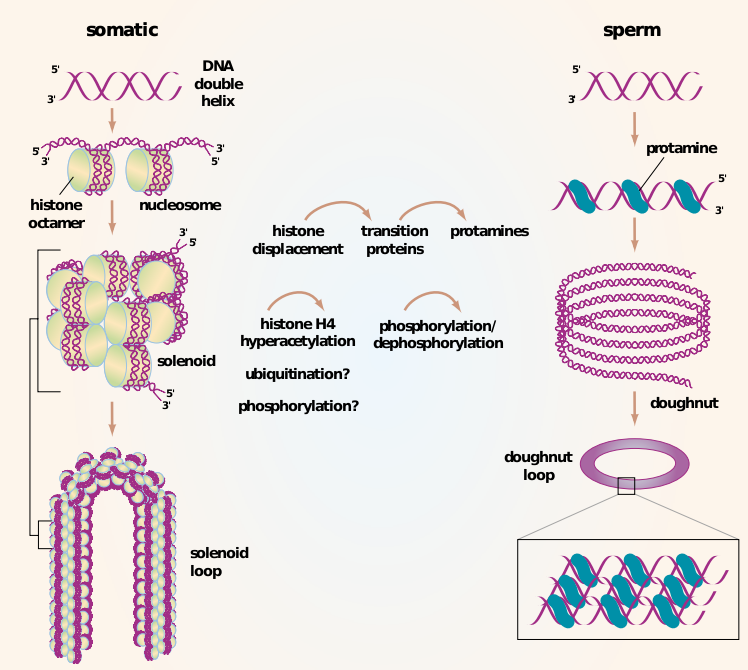
\includegraphics[scale=.55]{figure/noyau} 

}

\caption[Schéma de la compaction de l’ADN dans les cellules somatiques et dans les spermatozoïdes]{\textbf{\emph{Schéma de la compaction de l'ADN dans les
cellules somatiques et dans les spermatozoïdes} d'après
{[}\protect\hyperlink{ref-Braun2001}{30}{]}} : Dans les cellules
somatiques, l'ADN est enroulé sous forme de nucléosome. Les nucléosomes
vont s'agencer entre eux pour former un solénoïde qui sera attaché à la
matrice nucléaire par sa base. Dans le noyau spermatique les nucléosomes
sont remplacés par des protamines qui vont compacter l'ADN sous forme de
``\emph{doughnut}''. Le remplacement des histones est facilité par des
acétylations, des ubiquitinations et des phosphorylations.}\label{fig:noyau}
\end{figure}











\newpage

\subsection{Le flagelle}\label{le-flagelle}

Le flagelle représente la queue du spermatozoïde. Celui-ci permet, par
mouvements d'oscillation à haute vitesse, le déplacement du
spermatozoïde. Cette mobilité est générée par un cytosquelette interne
extrêmement conservé durant l'évolution appelé l'axonème. Celui-ci est
composé de neuf doublets de microtubules périphériques et de deux
doublets internes {[}\protect\hyperlink{ref-Inaba2003}{31}{]}
(\textbf{Figure : }\ref{fig:pictaxoneme}), on parle alors de structure
``9 + 2''. Les doublets externes sont reliés entre eux par des ponts de
nexine et au doublet central par des ponts radiaires. Les doublets
externes sont également reliés entre eux par les complexes protéiques
qui forment les dynéines externes et internes. Ce sont ces protéines qui
en exerçant une contraction alternée permettent le mouvement du
spermatozoïde.







\begin{figure}

{\centering 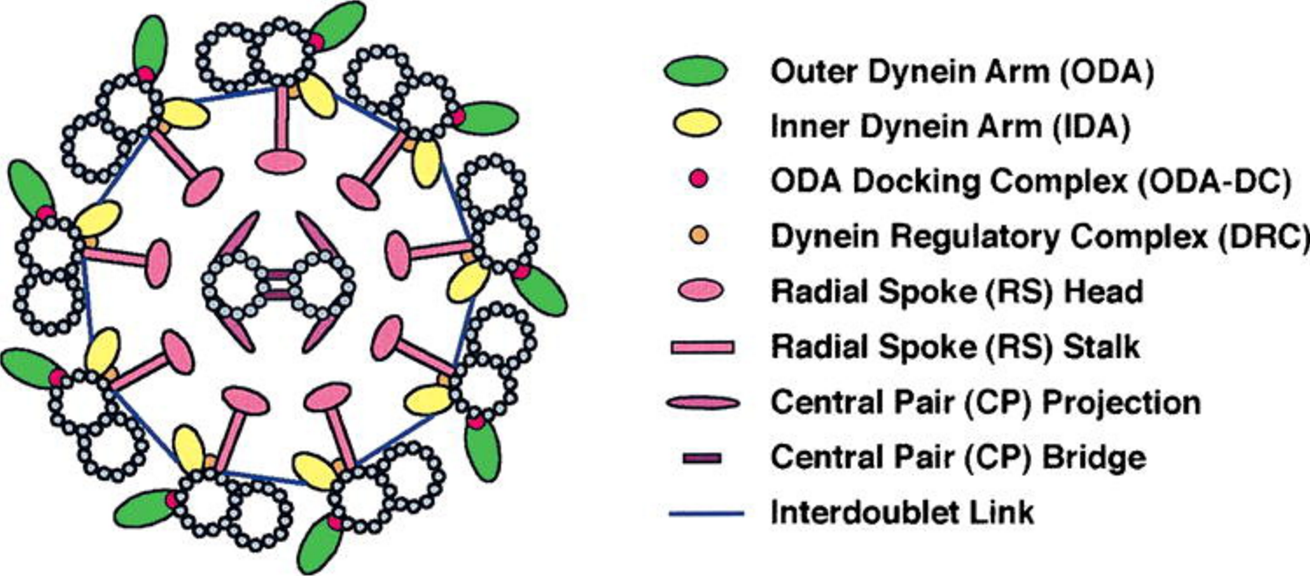
\includegraphics[scale=.3]{figure/axoneme} 

}

\caption[Structure simplifiée de l'axonème]{\textbf{\emph{Structure simplifiée de l'axonème}
d'après {[}\protect\hyperlink{ref-Inaba2003}{31}{]}} : L'axonème est
constitué de neuf doublets de microtubules périphériques reliés entre
eux par des liens de nexine et d'un doublet central relié aux doublets
périphériques par des ponts radiaires.}\label{fig:pictaxoneme}
\end{figure}

Le flagelle du spermatozoïde peut être divisé en trois parties
distinctes (\textbf{Figure : }\ref{fig:flagelle}) :

\begin{enumerate}
\def\labelenumi{\arabic{enumi}.}
\tightlist
\item
  \textbf{La pièce intermédiaire} : elle fait jonction avec la tête du
  spermatozoïde. Elle est composée de la gaine de mitochondrie qui
  fournira une partie de de l'énergie nécessaire au battement
  flagellaire (grâce à la phosphorylation oxydative qui produit de
  l'ATP). L'axonème qui se prolonge dans la pièce principale est un
  ensemble de neuf faisceaux de fibres denses.
\end{enumerate}

\newpage

\begin{enumerate}
\def\labelenumi{\arabic{enumi}.}
\setcounter{enumi}{1}
\tightlist
\item
  \textbf{La pièce principale} : ici, la gaine de mitochondrie a disparu
  ainsi que deux des faisceaux de fibres denses présents dans la pièce
  intermédiaire. On note cependant la présence d'une structure
  supplémentaire, la gaine fibreuse. Cette gaine entoure l'axonème et
  comporte deux épaississements diamétralement opposés, appelés colonnes
  longitudinales sur lesquelles s'insèrent les fibres denses 3 et 8.
  C'est le long de la gaine fibreuse qu'est produit la majorité de
  l'énergie nécessaire au glissement des microtubules
  {[}\protect\hyperlink{ref-Eddy2007}{32}{]}.\\
\item
  \textbf{La pièce terminale} : elle est située au niveau de l'extrémité
  distale du flagelle et ne contient que l'axonème
  {[}\protect\hyperlink{ref-Inaba2003}{31}{]}.
\end{enumerate}

\begin{figure}

{\centering 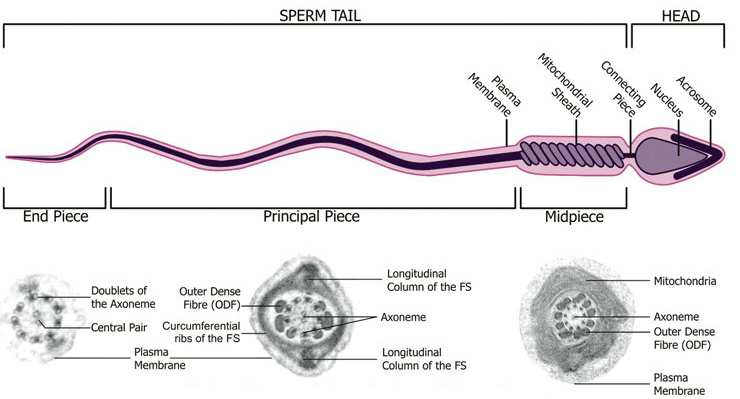
\includegraphics[scale=.55]{figure/sperm2} 

}

\caption[Structure du flagelle d’un spermatozoïde]{\textbf{\emph{Structure du flagelle d'un spermatozoïde}
d'après {[}\protect\hyperlink{ref-Borg2010}{33}{]}} : Coupes
transversales en microscopie électronique. Le flagelle se compose de
trois parties : la pièce intermédiaire, contenant les mitochondries, la
pièce principale et la pièce terminale. L'axonème, en position centrale,
parcours tout le flagelle. Des structures périaxonèmales sont
observables : les fibres denses dans la pièce intermédiaire et
principale, et la gaine fibreuse dans la pièce principale seulement.}\label{fig:flagelle}
\end{figure}










\newpage

\section{L'infertilité masculine}\label{linfertilite-masculine}

L'organisation mondiale de la santé définie l'infertilité comme étant :
``\emph{une pathologie du système reproductif définie par l'échec d'une
grossesse clinique après 12 mois ou plus de rapports sexuels réguliers
non protégés}''
(\href{http://www.who.int/reproductivehealth/topics/infertility/definitions/en/}{\texttt{Who.int.\ 2013-03-19.\ Retrieved\ 2013-06-17}}).
L'étude de l'infertilité représente un des enjeux scientifique et
médical majeur de ces dernières années. On estime qu'environ 10 à 15\%
des couples humains font face à des problèmes d'infertilité soit plus de
70 millions de personnes dans le monde
{[}\protect\hyperlink{ref-Boivin2007a}{34}{]}. Dans la moitié des cas,
la cause sous-jacente serait masculine. On estime que les facteurs
causaux sous-jacents de l'infertilité masculine peuvent être attribués à
des toxines environnementales, des troubles systémiques tels que la
maladie hypothalamo-hypophysaire, les cancers testiculaires et l'aplasie
des cellules germinales. Les facteurs génétiques, y compris les
aneuploïdies et les mutations de gènes uniques, contribuent également à
l'infertilité masculine. Cependant, aucune cause n'est identifiée dans
près de la moitié des cas. Comme nous avons pu le voir, la
spermatogenèse est une succession de processus complexes qui s'effectue
de manière coordonnée ; de fait la moindre altération génétique
affectant une seule de ces étapes est susceptible d'entraîner un
phénotype d'infertilité
{[}\protect\hyperlink{ref-Grudzinskas1995}{35}{]}.

\subsection{Les différents phénotypes d'infertilité
masculine}\label{les-differents-phenotypes-dinfertilite-masculine}

Chez l'homme, l'infertilité est associée à une altération quantitative
et / ou qualitative des spermatozoïdes présents dans l'éjaculat.
L'ensemble de ces altérations peut être détecté et quantifié dans des
laboratoires spécialisés, par réalisation d'un spermogramme. Au cours de
celui-ci, plusieurs critères tels que le volume de sperme sécrété, son
pH, la quantité et la vitalité des spermatozoïdes qu'il contient seront
évalués. La proportion de cellules immatures sera elle aussi analysée.
Ces cellules rondes, se retrouvent à la fois dans l'éjaculat des
individus ayant une quantité de spermatozoïdes ``normale''
{[}\protect\hyperlink{ref-Michael1937}{36}{]}, chez les individus
présentant une quantité basse de spermatozoïdes
{[}\protect\hyperlink{ref-MacLeod1970}{38},
\protect\hyperlink{ref-Tomlinson1993}{39}{]} ou en étant dépourvu
{[}\protect\hyperlink{ref-Kurilo}{40}{]}. Cependant, leur nombre
augmente tandis que la quantité de spermatozoïde diminue
{[}\protect\hyperlink{ref-SPERLING1971}{41}{]}.

\newpage

\subsubsection{Anomalies liées à la quantité
spermatique}\label{infquant}

Chez l'humain, l'arrêt de la spermatogénèse est défini comme
l'incapacité des cellules spermatogénétiques à devenir des
spermatozoïdes matures. Elle peut survenir à n'importe quelle étape de
la formation des cellules germinales. Les blocages méiotiques, au stade
de spermatocyte I, sont les plus fréquents, suivis par l'arrêt au niveau
des spermatides et moins fréquemment au niveau des spermatogonies
{[}\protect\hyperlink{ref-Girgis}{42}{]}.

\begin{enumerate}
\def\labelenumi{\arabic{enumi}.}
\item
  \textbf{L'oligozoospermie} : l'oligozoospermie est définie comme un
  phénotype d'infertilité masculine caractérisé par une production
  inférieure à 15 millions de spermatozoïdes par ml de sperme
  {[}\protect\hyperlink{ref-Cooper2010}{43}{]}. Un arrêt de la
  spermatogénèse a été observé dans 4 à 30\% des biopsies testiculaires
  des hommes présentant une oligospermie sévère
  {[}\protect\hyperlink{ref-Colgan1980}{44}--\protect\hyperlink{ref-WONG1973}{47}{]}.
  Cet arrêt a longtemps été considéré comme sans espoir pour les couples
  désirant concevoir, jusqu'à l'émergence de l'injection mécanique d'un
  spermatozoïde dans l'ovocyte appelé \emph{intracytoplasmic sperm
  injection} (ICSI) {[}\protect\hyperlink{ref-Palermo1992}{48}{]}.
\item
  \textbf{L'azoospermie} : comme l'oligozoospermie, l'azoospermie est un
  phénotype d'infertilité masculine cette fois-ci caractérisé par
  l'absence totale de spermatozoïdes dans l'éjaculat. On distingue des
  causes excrétoires empêchant l'excrétion des spermatozoïdes, on parle
  alors d'azoospermie obstructive et des causes sécrétoires, les plus
  fréquentes, accompagnées d'un défaut de la spermatogenèse, on parle
  alors d'azoospermie non-obstructive.
\end{enumerate}

\subsubsection{Anomalies liées à la
morphologie}\label{anomalies-liees-a-la-morphologie}

Ces anomalies sont observables en effectuant un spermocytogramme.
Plusieurs classifications ont été établies. Cependant, c'est la
classification de David modifiée (\textbf{Table :}
\ref{fig:anomaliemorphosperm}) qui est la plus repandue en France. Pour
ce faire, on procède généralement à une observation de 100
spermatozoïdes au cours de laquelle l'ensemble des anomalies observées
est relevé et quantifié permettant ainsi de définir un index d'anomalies
multiples (nombre total d'anomalies/nombre de spermatozoïdes anormaux)
révélant le nombre moyen d'anomalies par spermatozoïdes.

\newpage  

\begin{figure}

{\centering \includegraphics[scale=.75]{figure/tab_sperm_defect} 

}

\caption[Classification morphologique de spermatozoïdes humains normaux et anormaux]{\textbf{\emph{Classification morphologique de
spermatozoïdes humains normaux et anormaux} d'après
{[}\protect\hyperlink{ref-Auger2001}{49}{]}}.}\label{fig:anomaliemorphosperm}
\end{figure}





\newpage

\subsubsection{Anomalies liées à la
mobilité}\label{anomalies-liees-a-la-mobilite}

Le succès du passage du spermatozoïde le long du tractus génitale
féminin dépend en grande partie de la mobilité et de la vitesse du
spermatozoïde {[}\protect\hyperlink{ref-Lindholmer1974}{50},
\protect\hyperlink{ref-Bjorndahl2010}{51}{]}. La vitesse moyenne d'un
spermatozoïde étant de 25 \(\upmu\)m/s. Une mauvaise mobilité observée
dans plus de 50\% des spermatozoïdes éjaculés se révèle être un
prédicteur de l'échec de la fécondation
{[}\protect\hyperlink{ref-Aitken1985}{52}{]}.

\subsection{La génétique de
l'infertilité}\label{la-genetique-de-linfertilite}

Comme il a déjà été dit, il est estimé que 10 à 15\% des couples humains
font face à des problèmes d'infertilité. Par ailleurs, 30\% des
infertilités restent inexpliqués et près de 40\% ont des causes
incertaines. Ainsi, l'infertilité masculine d'origine génétique pourrait
concerner près d'un homme sur quarante
{[}\protect\hyperlink{ref-Tuttelmann2011}{53}{]}.

\subsubsection{Les causes fréquentes}\label{les-causes-frequentes}

\begin{enumerate}
\def\labelenumi{\arabic{enumi}.}
\tightlist
\item
  \textbf{Les microdélétions du chromosome Y} : le chromosome Y est un
  petit chromosome atteignant une taille d'environ 53 Mb. Il est porteur
  de 78 gènes principalement impliqués dans la différentiation sexuelle
  masculine et la spermatogenèse
  {[}\protect\hyperlink{ref-Skaletsky2003}{54}{]}. De fait, le
  chromosome Y représente une région d'intérêt évidente dans l'étude de
  facteurs génétiques liés à l'infertilité masculine. L'évolution des
  technologies a permis de mettre en évidence des délétions invisibles
  au caryotype dans la région du facteur AZF (\emph{Azoospermia
  Factor}). Cette région peut être subdivisée en trois sous-parties,
  AZFa, AZFb et AZFc (\textbf{Figure :} \ref{fig:chry}). Depuis
  plusieurs années, de nombreuses séries de patients azoospermiques ou
  oligozoospermiques ont été étudiées et publiées et tendent à montrer
  que les microdélétions du chromosome Y seraient responsables de 10\%
  des cas d'azoospermie non-obstructive et chez 5\% des cas
  d'oligozoospermie sévère (\textless{}5 millions de spermatozoïdes/ml)
  {[}\protect\hyperlink{ref-Hotaling2014}{55}{]}.
\end{enumerate}

\newpage

\begin{figure}

{\centering 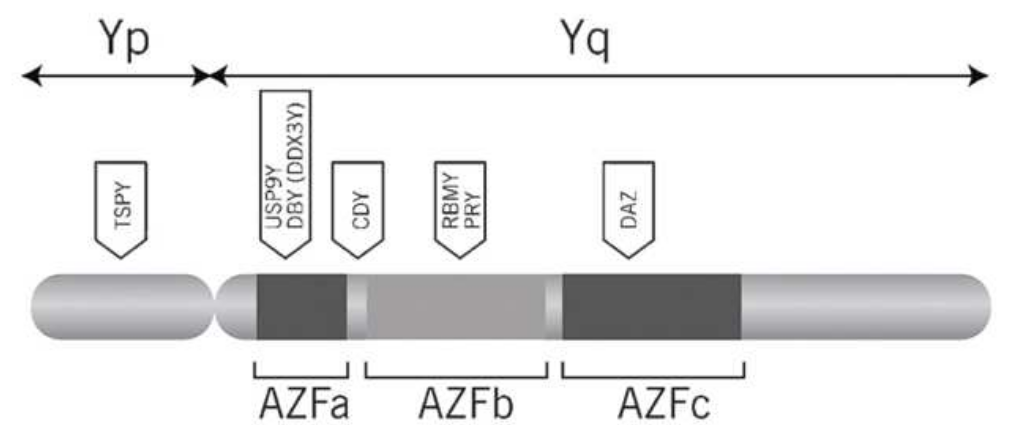
\includegraphics[scale=.45]{figure/chromozomeY} 

}

\caption[Représentation schématique du chromosome Y]{\textbf{\emph{Représentation schématique du chromosome Y}
adapté d'après {[}\protect\hyperlink{ref-OFlynnOBrien2010}{56}{]}} :
Visualisation la région AZF ainsi que des trois sous-régions AZF a, b, c
et des principaux gènes compris dans chacune des sous-régions.}\label{fig:chry}
\end{figure}






\begin{enumerate}
\def\labelenumi{\arabic{enumi}.}
\setcounter{enumi}{1}
\tightlist
\item
  \textbf{Anomalies chromosomiques} : des anomalies chromosomiques de
  nombre ou de structure impliquant les autosomes ou, le plus souvent,
  les gonosomes, peuvent être impliquées dans des cas d'infertilité
  masculine. Le pourcentage d'individus concernés varie entre 2 et 8\%
  et peut atteindre 15\% pour les patients azoospermiques soit 10 à 20
  fois la fréquence retrouvée dans la population générale
  {[}\protect\hyperlink{ref-Ravel2006}{57}{]}.

  \begin{enumerate}
  \def\labelenumii{\alph{enumii}.}
  \item
    \textbf{Syndrome de Klinefelter} : le syndrome de Klinefelter (ou
    46, XXY) fut décrit pour la première fois en 1942 par Harry F.
    Klinefelter. Il décrit une affection due à la présence d'un
    chromosome X supplémentaire suite à une erreur de ségrégation des
    chromosomes au moment de la méiose. Sa prévalence dans la population
    générale est estimée à environ 1 sur 1200 (1 homme sur 600)
    {[}\protect\hyperlink{ref-Bojesen2011}{58}{]} mais elle est environ
    50 fois supérieure chez les patients infertiles azoospermiques
    {[}\protect\hyperlink{ref-Gekas2001}{59}{]}.
  \item
    \textbf{Les anomalies de structure} : les translocations et les
    inversions sont les anomalies de structure retrouvées le plus
    fréquemment chez les patients infertiles.

    \begin{enumerate}
    \def\labelenumiii{\roman{enumiii}.}
    \tightlist
    \item
      La translocation est définie comme l'échange de matériel génétique
      entre deux chromosomes non homologues. On en distingue deux types,
      les translocations réciproques et les translocations
      robertsonniennes. Les premières (\textbf{Figure :}
      \ref{fig:figtranslocation} - \textbf{A}) décrivent un échange
      équilibré entre deux mêmes segments chromosomiques de deux
      chromosomes différents. Elles sont retrouvées 4 à 10 fois plus
      fréquemment chez les patients infertiles que dans la population
      générale {[}\protect\hyperlink{ref-Elliott1997}{60}{]}. Les
      secondes (\textbf{Figure :} \ref{fig:figtranslocation} -
      \textbf{B}) impliquent deux chromosomes acrocentriques et sont
      caractérisées par la fusion entre les brins longs de deux
      chromosomes, les brins courts étant perdus. Elles sont retrouvées
      chez 1.6\% des patients oligozoospermiques et 0.09\% des patients
      azoospermiques {[}\protect\hyperlink{ref-OFlynnOBrien2010}{56}{]}.
    \end{enumerate}
  \end{enumerate}
\end{enumerate}







\begin{figure}

{\centering \includegraphics[scale=.55]{figure/translocation} 

}

\caption[Les différents types de translocation]{\textbf{\emph{Les différents types de
translocation} d'après
\href{http://www.embryology.ch/francais/kchromaber/abweichende03.html}{embryology.ch}}
: \textbf{A} : La translocation réciproque. \textbf{B} : La
translocation robertsonniènne}\label{fig:figtranslocation}
\end{figure}

\begin{enumerate}
\def\labelenumi{\roman{enumi}.}
\setcounter{enumi}{1}
\item
  Les inversions chromosomiques caractérisent le mécanisme de cassure
  d'un fragment de chromosome suivi de son retournement à 180° et sa
  réintégration à la même position. Ces inversions vont gêner
  l'appariement des chromosomes homologues (formation d'une boucle
  d'inversion) pendant la méiose et sont, comme les translocations,
  retrouvées plus fréquemment chez les patients infertiles que dans la
  population générale {[}\protect\hyperlink{ref-Krausz2000}{61}{]}.

  \begin{enumerate}
  \def\labelenumii{\alph{enumii}.}
  \setcounter{enumii}{2}
  \tightlist
  \item
    \textbf{Autres anomalies chromosomiques} : parmi les anomalies
    chromosomiques responsables d'infertilité masculine, on peut par
    exemple citer les hommes de formule 46,XX. Ces patients sont
    généralement totalement infertiles et présentent une azoospermie par
    absence des sous- régions AZF a, b et c
    {[}\protect\hyperlink{ref-Vorona2007}{62}{]} bien qu'ils aient un
    phénotype masculin normal. Ces anomalies sont souvent le fait de la
    translocation du gène SRY sur un des chromosomes X du patient.
  \end{enumerate}
\end{enumerate}

\begin{enumerate}
\def\labelenumi{\arabic{enumi}.}
\setcounter{enumi}{2}
\tightlist
\item
  \textbf{Mutations du gène \emph{CFTR} }: l'identification du gène
  \emph{CFTR} (\emph{Cystic Fibrosis Transmembrane conductance
  Regulator}) chez les patients atteints de mucoviscidose et présentant
  une agénésie bilatérale des canaux déférents (ABCD) a permis
  d'associer ce gène au phénotype d'azoospermie obstructive. Cette
  malformation serait responsable de 2\% des cas d'infertilité masculine
  et de 25\% des cas d'azoospermie obstructive
  {[}\protect\hyperlink{ref-Yu2012}{63}{]}.
\end{enumerate}

Bien que la prévalence de ces anomalies génétiques varie en fonction du
phénotype concerné, il est estimé que ces défauts sont seulement
retrouvés chez 5\% des cas d'infertilité masculine, tous phénotypes
confondus. Cette observation suggère fortement l'implication de nombreux
autres gènes encore inconnus dans les différents phénotypes
d'infertilité masculine.

\newpage

\subsubsection{Les nouveaux gènes}\label{les-nouveaux-genes}

\begin{enumerate}
\def\labelenumi{\arabic{enumi}.}
\item
  \textbf{Les anomalies quantitatives} : une analyse de trois familles
  par séquençage \protect\hyperlink{ngs}{haut-débit} a permis
  d'identifier trois gènes \emph{MEIOB}, \emph{TEX14} et \emph{DNAH6}
  impliqués dans un phénotype d'azoospermie ; de même une étude de 2016
  démontre l'association de trois variants dans la séquence codante du
  gène \emph{RAD21L} en se basant sur une étude statistique effectuée
  sur 38 japonais présentant un arrêt de la fertilité et 200 contrôles
  {[}\protect\hyperlink{ref-Minase2017}{64}{]}. De même, plusieurs
  variants dans le gène \emph{TEX111} et \emph{SYC1} on été décrits
  comme entrainant un arrêt de la méiose
  {[}\protect\hyperlink{ref-Yatsenko2015}{65}--\protect\hyperlink{ref-Maor-Sagie2015}{67}{]}.
\item
  \textbf{Les anomalies morphologiques liées à la tête du spermatozoïde}
  :

  \begin{enumerate}
  \def\labelenumii{\alph{enumii}.}
  \tightlist
  \item
    \textbf{La macrozoospermie} : Ce phénotype d'infertilité masculine
    rare est caractérisé par la présence de 100\% des spermatozoïdes de
    l'éjaculat présentant une tête anormalement grosse ainsi que
    plusieurs flagelles. Il fut observé pour la première fois en 1978
    {[}\protect\hyperlink{ref-Nistal}{68}{]}, mais ce n'est qu'en 2007
    qu'une explication génétique fut enfin trouvée. Une étude portant
    sur 14 patients nord-africains a permis d'identifier la délétion
    c144delC du gène \emph{AURKC} (\emph{Aurora kinase C}) comme
    responsable du phénotype de l'ensemble des individus de l'étude
    {[}\protect\hyperlink{ref-Dieterich2007}{69}{]}. Depuis, d'autres
    études ont permis d'associer d'autres variants sur ce même gène à ce
    phénotype {[}\protect\hyperlink{ref-BenKhelifa2011}{70}{]}. Des
    anomalies du gène \emph{AURKC} seraient ainsi responsables d'environ
    83.7\% des cas macrozoospermie chez des patients non apparentés
    {[}INSERT REF{]}. Le gène AURKC, étant impliqué dans la méiose,
    conduit lorsqu'il est muté à un blocage de la première division
    méiotique, entraînant la production de spermatozoïdes tétraploïdes,
    c'est à dire, portant une quantité de matériel génétique quatre fois
    supérieure à la normale
    {[}\protect\hyperlink{ref-Dieterich2009}{71}{]}.\\
  \item
    \textbf{La globozoospermie} : La globozoospermie est aussi un
    phénotype rare d'infertilité dont la prévalence est estimée à de
    0,1\%. Il fut identifié pour la première fois en 1971 et est
    caractérisé par la présence dans l'éjaculat d'une majorité de
    spermatozoïdes dépourvus d'acrosome, empêchant le spermatozoïde de
    franchir la zone pellucide de l'ovocyte et compromettant ainsi la
    fécondation
    {[}\protect\hyperlink{ref-Dam2006}{72}--\protect\hyperlink{ref-Holstein1973}{74}{]}.
    En 2007, une étude familiale a permis de lier ce phénotype à la
    mutation c.848G\textgreater{}A dans le gène \emph{SPATA16}
    (\emph{spermatogenesis-associated protein 16})
    {[}\protect\hyperlink{ref-Dam2007a}{75}{]} dont la protéine va, au
    cours de la spermatogénèse, fusionner avec les vésicules
    proacrosomales pour former l'acrosome
    {[}\protect\hyperlink{ref-Dam2007a}{75},
    \protect\hyperlink{ref-Lu2006}{76}{]}. Plus tard, en 2011, une étude
    portant sur 20 patients tunisiens permit d'identifier une délétion
    homozygote de 200 kb emportant la totalité du gène \emph{DPY19L2}
    (\emph{Dpy-19 Like 2}) chez 15 des 20 patients
    {[}\protect\hyperlink{ref-Harbuz2011}{77}{]}. cf
    \protect\hyperlink{globo}{globo}\\
  \item
    \textbf{Spermatozoïdes acéphaliques} : Ce phénotype rapporté
    plusieurs fois
    {[}\protect\hyperlink{ref-Chemes2010}{78}--\protect\hyperlink{ref-Chemes1987}{80}{]}
    caractérise les patients présentant des spermatozoïdes dépourvus de
    tête dans leur éjaculat. Une étude récente a pu lier ce phénotype à
    une mutation c.824C\textgreater{}T homozygote ainsi qu'à deux
    variants hétérozygotes composites c.1006C\textgreater{}T et
    c.485T\textgreater{}A dans le gène \emph{SUN5}
    {[}\protect\hyperlink{ref-Zhu2016}{81}{]} qui avait précédemment été
    décrit comme localisant à la jonction noyau / flagelle du
    spermatozoïde {[}\protect\hyperlink{ref-Yassine2015}{82}{]}.
  \end{enumerate}
\item
  \textbf{Le phénotype MMAF} : Le phénotype MMAF (\emph{Multiple
  morphological abnormalities of the sperm flagella}) décrit les
  patients atteints d'asthenozoospermie dont les spermatozoïdes
  présentent de multiples anomalies morphologiques touchant en
  particulier les flagelles. Plus précisément, ce phénotype décrit les
  asthenozoospermie résultant d'une mosaïque d'anomalies morphologiques
  au niveau du flagelle tel que l'absence totale de flagelle, des
  flagelles enroulés, courts, anguleux\ldots{}
  {[}\protect\hyperlink{ref-Coutton2015}{83},
  \protect\hyperlink{ref-BenKhelifa2014}{84}{]}. Récemment, le gène
  \emph{DNAH1} (\emph{Dynein Axonemal Heavy Chain 1}) codant pour une
  dynéine de la chaine lourde de l'axonème a été retrouvé muté chez près
  d'un patient sur trois dans sa cohorte comportant 18 patients
  {[}\protect\hyperlink{ref-BenKhelifa2014}{84}{]}. Deux autres études
  ont retrouvé des mutations dans le gène \emph{DNAH1} chez des patients
  venant de Chine, d'Iran et d'Italie, laissant suggérer que ce gène est
  l'un des acteurs majeurs dans le syndrome MMAF
  {[}\protect\hyperlink{ref-Wang2017}{85},
  \protect\hyperlink{ref-Amiri-Yekta2016}{86}{]}.
\item
  \textbf{Les échecs de fécondation du spermatozoïde} : Au moment de la
  fécondation, l'activation ovocytaire repose sur le relargage par le
  spermatozoïde de ``facteurs spermatiques'' qui déclenchent un signal
  de calcium, constitué d'oscillations Ca\textsuperscript{2+}. Ce
  processus est médié par une protéine spécifique du spermatozoïde,
  \emph{la phospholipase C Zeta 1} (PLC\(\zeta 1\)) codée par le gène
  \emph{PLCZ1} {[}\protect\hyperlink{ref-Nomikos2013}{87},
  \protect\hyperlink{ref-Amdani2013}{88}{]}. Plusieurs cas d'échec
  d'activation ovocytaire ont été liés à l'absence ou à la mauvaise
  localisation de la protéine PLC\(\zeta1\). Malgré cela, aucune preuve
  génétique directe n'avait été reportée jusqu'à récemment où deux
  mutations au sein du gène \emph{PLC}\(\zeta\)\emph{1} furent
  retrouvées chez un patient
  {[}\protect\hyperlink{ref-Heytens2009}{89}{]} et un peu plus tard une
  mutation homozygote chez deux frères consanguins
  {[}\protect\hyperlink{ref-Escoffier2016}{90}{]}.
\end{enumerate}

\newpage  

\section{Les techniques d'analyses
génétiques}\label{les-techniques-danalyses-genetiques}

L'acide désoxyribonucléique (ADN) a été identifié comme étant le porteur
de l'information génétique par Oswald Theodore Avery en 1944. Sa
structure en double hélice composée par quatre bases, la thymine (T),
l'adénine (A), la guanine (G) et la cytosine (C) fut caractérisée en
1953 par James D. Watson et Francis Crick. Cependant, l'existence
``d'entités d'information génétiques discrètes'' que sont les gènes fut
suggéré dès la deuxième moitié du XIX\textsuperscript{ième} siècle grâce
aux travaux de Gregor Mendel portant sur l'hérédité de certains traits
chez le pois. Depuis, de nombreuses méthodes permettant de lier le
phénotype d'un individu à son génotype ont vu le jour au gré des
améliorations technologiques.

\subsection{\texorpdfstring{Approche ``gènes
candidats''}{Approche gènes candidats}}\label{approche-genes-candidats}

L'approche ``gènes candidats''" consiste à rechercher des mutations chez
un patient dans un ou plusieurs gènes cibles. Le choix des gènes cibles
se fera en fonction de plusieurs critères. Le premier d'entre eux est
l'étude de gènes reliés à des phénotypes proches du phénotype étudié
dans différents modèles animaux et notamment murins. Dans ce cas, les
mutations seront recherchées sur le gène orthologue humain
{[}\protect\hyperlink{ref-DeBoer2015}{91}{]}. Une autre possibilité
consiste à rechercher des variants dans des gènes paralogues à un gène
précédemment identifié avec l'idée sous-jacente que leur structure
proche implique une fonction similaire. Enfin la dernière méthode
consiste à étudier des gènes connus comme étant des partenaires de gènes
déjà identifiés dans cette pathologie, en supposant que si un variant
dans un gène donné entraîne une pathologie, un variant dans un
partenaire de ce gène pourrait entraîner le même phénotype. Cette
approche est bien souvent infructueuse, ceci étant dû, en grande partie,
à l'hétérogénéité génétique des phénotypes étudiés, au nombre limité de
patients testés {[}\protect\hyperlink{ref-ElInati2012}{92}{]} et aux
connaissances souvent incomplètes sur le phénotype. De fait, cette
approche a quasiment disparu au profit des méthodes à haut débit que
sont les puces et le séquençage nouvelle génération (NGS). Néanmoins,
cette méthode compte à son actif plusieurs succès retentissants avec
dans le domaine de l'infertilité masculine, les gènes \emph{SYCP3},
\emph{SOHLH1} et \emph{NR5A1} entraînant tous les trois un phénotype
d'azoospermie
{[}\protect\hyperlink{ref-Miyamoto2003}{93}--\protect\hyperlink{ref-Bashamboo2010}{95}{]}.

\newpage

\subsection{Les puces}\label{les-puces}

Les puces à ADN furent initialement conçues dans le but de mesurer le
niveau de transcription des transcrits provenant de plusieurs milliers
de gènes lors d'une seule et unique expérience. Cette technologie a
ainsi permis de déterminer des patterns d'expression de gènes à un statu
physiologique donné. L'analyse des ``signatures'' d'expression a ainsi
permis de caractériser plusieurs cancers
{[}\protect\hyperlink{ref-Alon1999}{96}--\protect\hyperlink{ref-VantVeer2002}{99}{]},
mais aussi la réponse physiologique à plusieurs types de stimuli tel que
la prise de certains médicaments
{[}\protect\hyperlink{ref-Brachat2002}{100}{]}.

Suite à cela, l'usage des puces à ADN dans le domaine biomédical s'est
étendu pour ne plus être limité à la simple quantification de
l'expression génique. Ainsi, cette technologie a également été utilisée
afin de détecter des \emph{single nucleotide polymorphisms} (SNPs) au
sein de notre génome permettant notamment l'émergence du HapMap Project
qui recense les SNPs de plusieurs milliers d'individus
{[}\protect\hyperlink{ref-Cutler2001}{101}{]}. De même, l'utilisation
des puces à ADN a permis la détection de \emph{copy number variation}
(CNVs).

Pendant plus de 10 ans, la grande qualité des puces, l'existence de
protocoles d'hybridation standardisés ainsi que des algorithmes
d'analyses robustes ont fait des puces à ADN l'outil d'analyse génomique
le plus puissant avant l'arrivée du \protect\hyperlink{ngs}{séquençage
haut débit}

\newpage

\subsubsection{Les puces à expression}\label{les-puces-a-expression}

L'utilisation principale des puces à ADN a été de mesurer l'expression
des gènes dans un tissus donné. Dans cette application, l'ARN est
extrait des cellules d'intérêt puis est généralement converti en ADNc.
Dans un second temps, l'ADNc est hybridé à la puce qui subira par la
suite une étape de lavage. Pour finir, l'intensité de fluorescence est
mesurée à chaque spot de la puce et déterminera le niveau d'expression
d'un gène.

\begin{figure}

{\centering \includegraphics[scale=.9]{figure/expression_array} 

}

\caption[Représentation schématique des méthodes d'analyse d'expression génique par puce à ADN]{\textbf{\emph{Représentation schématique des méthodes
d'analyse d'expression génique par puce à ADN} d'après
{[}\protect\hyperlink{ref-Trevino2007}{102}{]}} : Présentation des
méthodes à double et à simple colorant, respectivement à gauche et à
droite. Pour les analyses à double colorant, une seule puce et
nécessaire, les échantillons de la référence et du test sont mis en
compétition sur la même puce, un signal de sortie vert indiquera une
surexpression chez le test tandis qu'un signal rouge indiquera une
sous-expression. Pour celles à simple colorant, deux puces sont
nécessaires, une première pour la référence et une seconde pour le test.
Les données des deux puces sont ensuite comparées pour déterminer quels
sont les gènes différentiellement exprimés. Dans le cas de la CGH array,
le principe est similaire, en remplaçant simplement l'ARNm par de
l'ADNg.}\label{fig:pictexparray}
\end{figure}
















\newpage

\subsubsection{Les puces à SNP, plateforme
génotypage}\label{les-puces-a-snp-plateforme-genotypage}

Bien que leur utilité principale ait été d'analyser l'expression des
gènes, les puces à ADN ont également été extrêmement utilisées comme
moyen de génotyper les SNP (\emph{single-nucleotide-polymorphism}). De
nombreuses méthodes ont été mises en place pour cela ; cependant la plus
employée est la méthode de discrimination allélique par hybridation
telle qu'elle est utilisée par Affymetrix
{[}\protect\hyperlink{ref-Wang1998}{103}{]} malgré le ``bruit de fond''
causé par l'hybridation non spécifique dont elle souffre (\textbf{Figure
:} \ref{fig:pictallelicdisc}).

\begin{figure}

{\centering \includegraphics[scale=.7]{figure/allelic_discrimination} 

}

\caption[Méthode de génotypage par discrimination allélique par hybridation]{\textbf{\emph{Méthode de génotypage par
discrimination allélique par hybridation} d'après
{[}\protect\hyperlink{ref-Bumgarner2013}{104}{]}} : Des sondes
complémentaires à chacun des allèles sont positionnées sur la puce.
L'ADN génomique fragmenté et labélisé est mis en contact de la puce.
Après nettoyage de la puce, l'analyse du signal émis par l'ADN génomique
permettra de déterminer si l'individu est homozygote pour cette allèle
(hybridation à une seule des deux sondes) ou bien hétérozygote pour
cette allèle (hybridation aux deux sondes).}\label{fig:pictallelicdisc}
\end{figure}











\newpage

\subsubsection{Les puces à indels}\label{les-puces-a-indels}

L'implication de réarrangements génomiques tel que des duplications,
translocations ou délétions dans divers pathologies est bien connue.
C'est afin de détecter ces réarrangements que la \emph{Comparative
Genomic Hybridization array} (CGH array) a été développée dès 1999
{[}\protect\hyperlink{ref-Brown1999}{105}{]}. Son principe est très
similaire à celui utilisé dans les puces à expression (\textbf{Figure :}
\ref{fig:pictexparray}) en remplaçant simplement l'ARN messager (ARNm)
par de l'ADN génomique (ADNg). Ainsi, la présence d'un CNV sera
facilement détectée en comparant le signal émis par un individu test
avec celui émis par un contrôle.

\subsubsection{Limitation}\label{limitation}

Bien que cette technologie ait été largement utilisée dans divers champs
d'applications, elle présente deux limitations principales.

\begin{enumerate}
\def\labelenumi{\arabic{enumi}.}
\item
  \textbf{Limitation n°1 :} Pour les génomes complexes (tel que les
  mammifères), il est difficile, si ce n'est impossible de
  \emph{designer} une puce ne permettant pas de l'hybridation non
  spécifique. En effet, la séquence d'une puce prévue pour détecter le
  gène ``A'' pourra également détecter les gènes ``B'', ``C'' et ``D''
  si ceux-ci présentent une forte homologie avec ``A'' Ce qui est
  particulièrement problématique dans le cas d'analyse de gènes d'une
  même famille.
\item
  \textbf{Limitation n°2 :} les puces détectent uniquement ce pour quoi
  elles ont été \emph{designer}. Ainsi, si la solution que l'on hybride
  sur la puce contient des séquences d'ADN ou d'ARN pour lesquelles il
  n'y a aucune sonde complémentaire sur la puce, celles-ci ne seront pas
  détectées. Cela peut avoir de grandes répercutions puisque par exemple
  dans le cas des puces à expression, les gènes qui n'ont pas encore été
  annotés risquent de ne pas être représentés sur la puce.
\end{enumerate}

\newpage

\hypertarget{ngs}{\subsection{Le séquençage NGS}\label{ngs}}

Le terme séquençage de l'ADN fait référence à l'ensemble des techniques
permettant de déterminer l'ordre des nucléotides A, T, C et G de
l'intégralité ou d'une partie d'une molécule d'ADN. Avant de parler des
nouvelles technologies de séquençage (NGS) faisons un bref historique du
séquençage de l'ADN. En 1977 Frederick Sanger développe une technologie
de séquençage d'ADN basée sur la méthode \emph{chain-termination}. Ce
procédé est désormais connu sous le nom de séquençage Sanger. D'autres
méthodes furent développées à la même période, notamment celle de Walter
Gilbert basée sur la modification chimique de l'ADN, cependant sa grande
efficience et sa faible utilisation de la radioactivité permirent au
séquençage Sanger de s'imposer comme référence dans la ``première
génération'' de séquenceur à application commerciale et de recherche.
Apparus en 1998, les instruments de séquençage automatique ainsi que les
logiciels associés utilisant le séquençage par capillarité et la
technologie Sanger furent les outils principaux qui permirent la
complétion du \emph{human genome project} en 2001
{[}\protect\hyperlink{ref-Collins2003}{106}{]}.

Contrairement à la méthode Sanger, le NGS est capable de ``\emph{lire}''
des fragments d'ADN provenant d'un génome \textbf{entier}. On parle
alors de séquençage de génomes entiers ou \emph{whole genome sequencing}
(WGS). Pour cela, la molécule d'ADN est ``coupée'' en plusieurs
fragments d'une taille donnée. Ce sont ensuite ces fragments qui seront,
après une étape d'amplification spécifique aux différentes plateformes,
séquencés simultanément. C'est pourquoi on parle souvent de séquençage
parallèle massif pour décrire le NGS. Le produit de ce séquençage est
appelé \emph{read}. Cette technologie est avantageuse de par la masse de
\emph{reads} qu'elle produit et par son faible coût par base séquencée
{[}\protect\hyperlink{ref-Metzker2010}{107}{]}. Ces caractéristiques ont
permis au séquençage Haut-débit d'être couramment utilisé dans le
domaine de la recherche clinique.

La taille des \emph{reads} obtenus par séquençage NGS est, hormis dans
le cas de la technologie PacBio, nettement inférieure à celle atteinte
par le séquençage Sanger. À l'heure actuelle, les \emph{reads} obtenus
par séquençage NGS ont une taille comprise entre 50 et 500 pb pour la
plupart des plateforme contre une taille d'environ 800 nucléotides
obtenus par Sanger (\textbf{Figure :} \ref{fig:pictreadPerRun}) ; c'est
pour cela que les résultats du séquençage NGS sont appelés des
\emph{reads} courts ou \emph{short reads}.\\
Étant donné que le NGS produit à l'heure actuelle des \emph{reads}
courts la notion de couverture est importante et représente l'un des
critères majeur à considérer dans l'analyse des données
{[}\protect\hyperlink{ref-Sims2014}{108}{]}. La couverture est définie
comme le nombre de \emph{reads} qui, après l'étape
\protect\hyperlink{lalignement}{d'alignement}, se chevauchent les uns
les autres au sein d'une région génomique spécifique. Par exemple, une
couverture de 30x pour le gène XXXX signifie que chaque nucléotide de ce
gène est chevauché par au moins 30 \emph{reads} distincts.

\newpage

\begin{figure}

{\centering 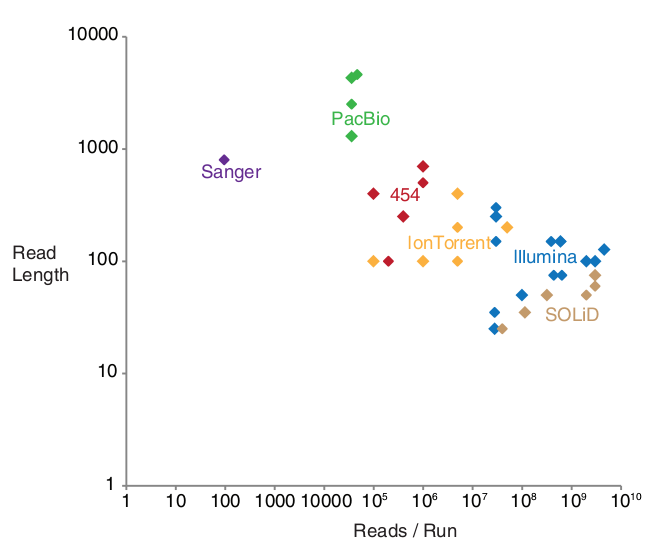
\includegraphics[scale=.55]{figure/read_per_run} 

}

\caption[Présentation de la taille des reads et du nombre de reads par run en fonction de la technologie de séquençage utilisée]{\textbf{\emph{Présentation de la taille des reads
et du nombre de reads par run en fonction de la technologie de
séquençage utilisée} d'après
{[}\protect\hyperlink{ref-Hodkinson2015}{109}{]}} : Chaque point
représente une plateforme de séquençage, la couleur détermine la marque
du séquenceur.}\label{fig:pictreadPerRun}
\end{figure}








\subsubsection{La capture des parties à séquencer, avantages et
inconvénients}\label{la-capture-des-parties-a-sequencer-avantages-et-inconvenients}

Pour de nombreuses applications, il peut être intéressant de ne
séquencer qu'une partie du génome et non pas son intégralité. Dans cette
sous partie de génome ciblé on peut trouver par exemple : une région
génomique spécifique à laquelle une pathologie a déjà été associée,
l'ensemble des exons de certains gènes candidats, ou encore
l'intégralité des exons de l'ensemble des gènes codant pour une
protéine. Dans ce dernier cas, on parle alors de séquençage exomique ou
\emph{whole exome sequencing} (WES). Les principaux avantages du WES par
rapport au WGS sont son coût réduit ainsi qu'une masse de données moins
importante à stocker et à analyser. En effet, l'ensemble de l'exome ne
représente qu'environ 1\% du génome entier. On considère cependant que
ces parties codantes contiennent plus de 90\% des anomalies responsables
de pathologies génétiques chez l'homme. Pour ces raisons, le WES est
considéré comme le standard dans le cadre de recherche sur des
pathologies génétiques et se révèle être un outil puissant pour
l'identification de variants associés à des pathologies
{[}\protect\hyperlink{ref-Ng2010}{110}{]}. Le procédé de séquençage est
identique au WGS, il est simplement précédé d'une étape d'enrichissement
au cours de laquelle les exons sont capturés par hybridation à des
sondes. De fait les exons capturés sont donc dépendants du kit de
capture utilisé, cette technique permet donc de séquencer uniquement les
exons connus et ciblés par les sondes. Il faut également noter que
depuis quelques années, plusieurs études ont remis en cause l'intérêt du
WES au profit du WGS, notamment car dans des conditions de séquençage
standards, la proportion des régions codantes, définies à la fois par
RefSeq et Ensembl, séquencée est plus importante dans le cas du WGS que
dans le WES {[}\protect\hyperlink{ref-Lelieveld2015}{111},
\protect\hyperlink{ref-Meienberg2016}{112}{]}. De plus le WES montre une
plus grande sensibilité au pourcentage de GC contenu dans la région à
séquencer et à la sélection des kits de capture utilisés
{[}\protect\hyperlink{ref-Meienberg2016}{112}{]}. Ainsi, bien que le WES
soit encore à l'heure actuelle le choix privilégié dans la majorité des
études, la réduction des coûts de séquençage et du stockage des données,
pourrait permettre prochainement au WGS de remplacer totalement le WES
ainsi que l'ensemble des techniques impliquant la capture de séquences
ciblées {[}\protect\hyperlink{ref-Meienberg2016}{112}{]}.

\subsubsection{L'amplification}\label{lamplification}

Dans la plupart des technologies, la phase de séquençage est précédée
par une étape d'amplification de l'ADN. Cette amplification se fait dans
la grande majorité des cas sur une surface solide excepté pour la PCR en
émulsion qui s'effectue en phase aqueuse. Elle permet d'obtenir dans une
région définie plusieurs milliers de copies du même fragment d'ADN,
appelés des clones. Cette étape assure que le signal émis lors du
séquençage pourra être distingué du bruit. Chacun de ces \emph{spots}
d'amplification appelés aussi centre de réaction, se retrouve donc être
le représentant d'un unique fragment d'ADN. Ceux-ci seront ensuite
séquencés parallèlement aux autres \emph{spots}. Une plateforme de
séquençage peut gérer plusieurs millions de ces centres de réactions
simultanément, séquençant ainsi plusieurs millions de molécules d'ADN en
parallèle, donnant ainsi le nom de séquençage massif en parallèle à ces
techniques. Cette étape d'amplification est généralement précédée d'une
phase de fragmentation de l'ADN. Cette fragmentation peut être physique,
enzymatique ou bien chimique. Ce sont les résidus d'ADN résultant de
cette fragmentation qui seront ensuite amplifiés. Il existe quatre
stratégies utilisées pour le clonage de l'ADN dans le cadre du NGS :

\begin{enumerate}
\def\labelenumi{\arabic{enumi}.}
\item
  \textbf{La PCR en émulsion ou emPCR} (\textbf{Figure :
  }\ref{fig:pictngsampli} - \textbf{a}) : Le patron d'ADN fragmenté
  simple brin est lié à une séquence adaptatrice complémentaire. Il est
  capturé par une gouttelette aqueuse appelée micelle contenant une
  bille recouverte d'adaptateur complémentaire à celui fixé sur le
  fragment d'ADN ainsi que tous les composants nécessaires à la réaction
  de PCR. En respectant un ratio nombre de molécules d'ADN / nombre de
  billes, on va fixer un seul fragment d'ADN sur chaque bille. Chacune
  de ces billes sera donc, en fin de réaction, recouverte par plusieurs
  milliers de copies de la même séquence d'ADN.
\item
  \textbf{L'amplification par pont sur face solide} (\textbf{Figure :
  }\ref{fig:pictngsampli} - \textbf{b}) : Les fragments d'ADN sont liés
  à des séquences adaptatrices et liés par une de leurs extrémités à une
  amorce fixée sur un support solide. Du fait de la dilution, les
  molécules d'ADN se trouvent éloignées les unes des autres. L'extrémité
  libre du fragment interagit avec les amorces situées à proximité
  formant une structure en pont, d'où le nom de PCR en pont ou
  \emph{bridge-PCR}. La PCR va alors synthétiser un deuxième brin
  complémentaire aux fragments immobilisés sur le support. En procédant
  à des cycles de température comme pour une réaction PCR classique, on
  obtient à l'emplacement de chaque molécule d'ADN un massif de
  molécules fixé sur la plaque, toutes identiques à la molécule
  initiale.
\item
  \textbf{Amplification par modèle mobile ou \emph{walking-template}
  }(\textbf{Figure : }\ref{fig:pictngsampli} - \textbf{c}) : L'ADN
  fragmenté est lié à un adaptateur et à une amorce complémentaire fixée
  sur un support solide. Le brin complémentaire du fragment sera
  synthétisé par PCR à partir de l'amorce fixée. La molécule double brin
  nouvellement formée sera ensuite partiellement dénaturée permettant à
  l'extrémité libre de se fixer à une séquence amorce voisine. Des
  amorces \emph{reverse} sont ensuite utilisées pour resynthétiser un
  fragment d'ADN libre à partir des fragments fixés sur le support.
\end{enumerate}

\newpage 

\begin{figure}

{\centering 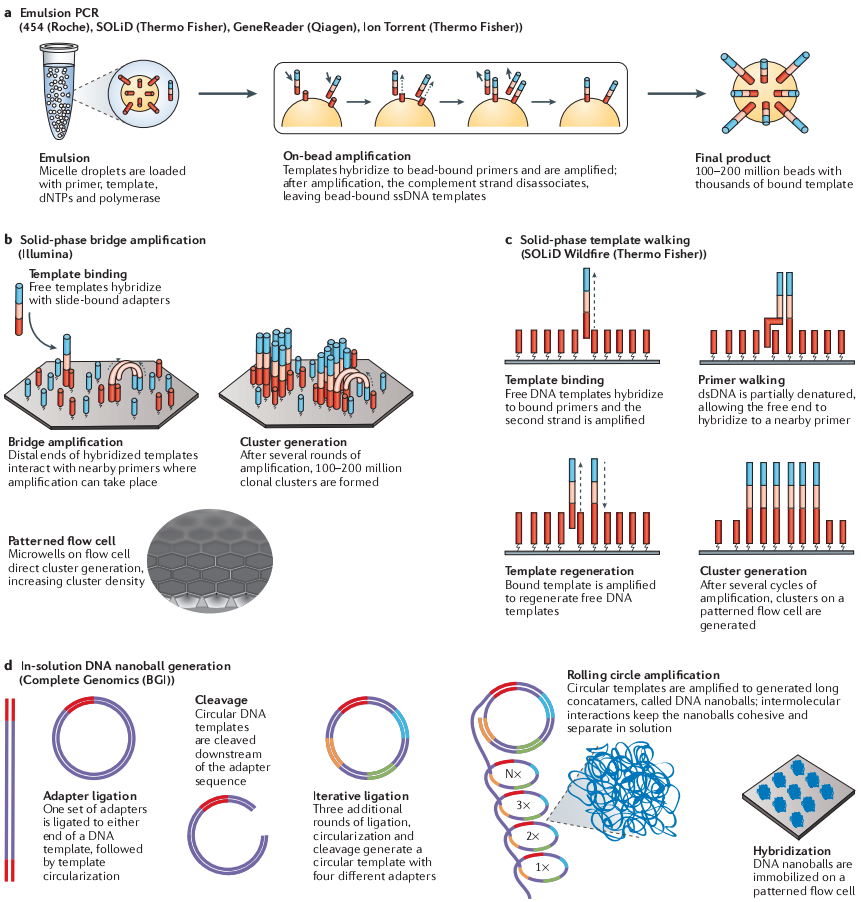
\includegraphics[scale=.455]{figure/ngs_amplification} 

}

\caption[Présentation des différentes stratégies d'amplification de l'ADN dans le cadre du NGS]{\textbf{\emph{Présentation des différentes stratégies
d'amplification de l'ADN dans le cadre du NGS} d'après
{[}\protect\hyperlink{ref-Goodwin2016}{113}{]}} : \textbf{a} : PCR en
émulsion. \textbf{b} : amplification par pont. \textbf{c} :
amplification par modèle mobile.}\label{fig:pictngsampli}
\end{figure}







\newpage

\subsubsection{La réaction de séquence}\label{la-reaction-de-sequence}

La réaction de séquence est l'étape suivant l'amplification. Ell
consiste à déterminer l'ordre dans lequel se succèdent les nucléotides
de l'ensemble des clones générés dans la phase d'amplification. Il
existe deux technologies principales permettant le séquençage de
\emph{reads} courts :

\begin{enumerate}
\def\labelenumi{\arabic{enumi}.}
\tightlist
\item
  \textbf{Séquençage par synthèse} (SBS) : Ce type de séquençage
  regroupe l'ensemble des méthodes utilisant l'ADN polymérase pour
  synthétiser de l'ADN. En 2016, Sahra Goodwin et ses collègues ont
  différenciés deux catégories de séquençage par synthèse
  {[}\protect\hyperlink{ref-Goodwin2016}{113}{]} :

  \begin{enumerate}
  \def\labelenumii{\alph{enumii}.}
  \tightlist
  \item
    \textbf{Terminaison par cycle réversible}, \emph{cyclic reversible
    termination} (CRT) (\textbf{Figure : }\ref{fig:pictcrtSeq}) : Cette
    méthode est caractérisée par l'utilisation de molécule dites
    terminatrices auxquelles le groupement \(\mathrm{3'-OH}\) est
    modifié de sorte à éviter l'élongation
    {[}\protect\hyperlink{ref-Guo2008}{114}{]}, on parlera de groupement
    \(\mathrm{3'-bloqué}\). Une amorce liée au fragment d'ADN permettra
    l'initialisation du processus de polymérisation. À chaque cycle, un
    mix comprenant l'ensemble des quatre désoxynucléotides (dNTPs),
    préalablement labélisés par un fluorophore \(\mathrm{3'-bloqué}\),
    est mis en contact du fragment. Après l'incorporation d'un unique
    dNTP au fragment, les dNTPs non liés sont éliminés et la nature du
    dNTP ajouté est identifiée grâce à son fluorophore. Le fluorophore
    et le groupement \(\mathrm{3'-bloqué}\) sont retirés permettant
    ainsi à un nouveau cycle de commencer.
  \end{enumerate}
\end{enumerate}

\begin{figure}

{\centering 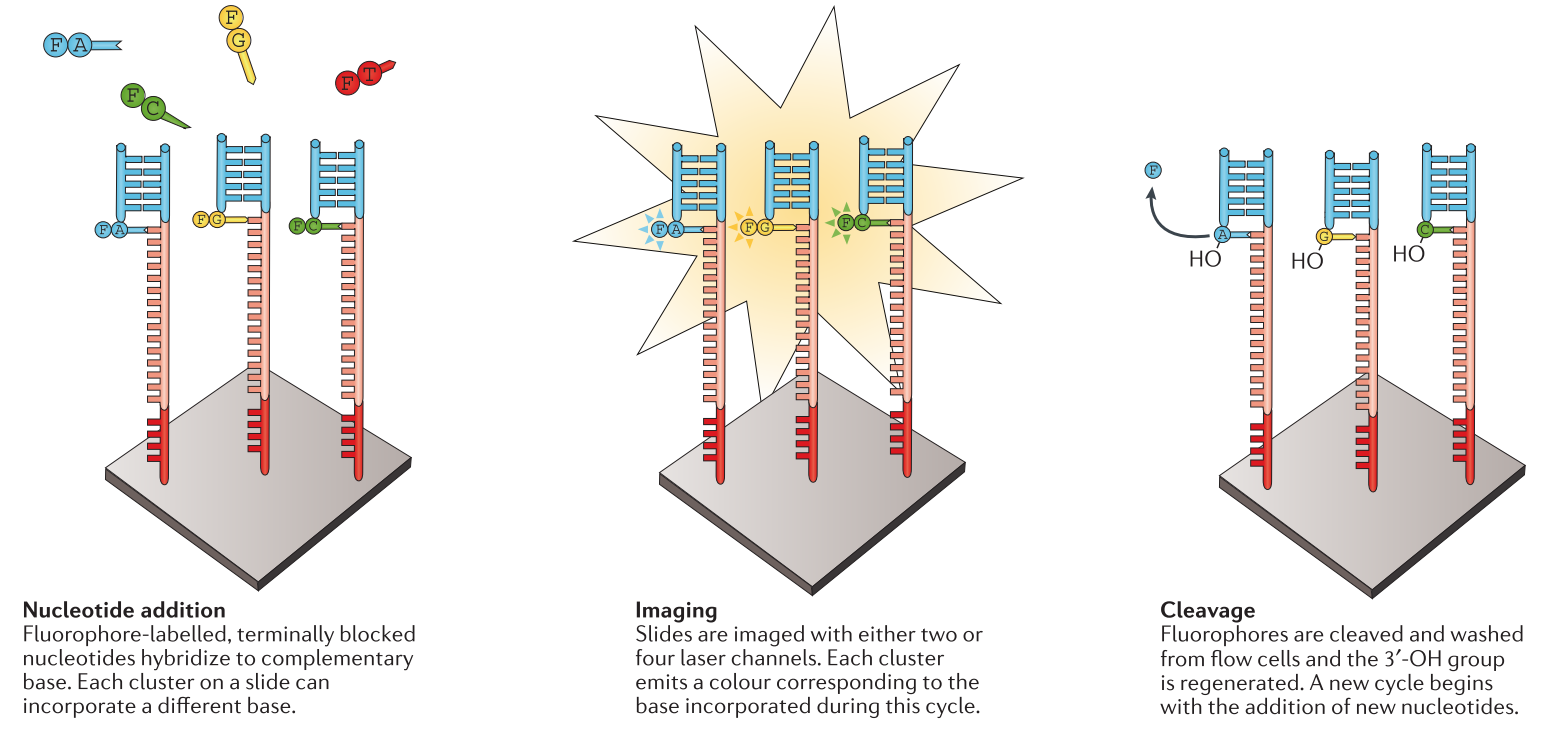
\includegraphics[scale=.24]{figure/CRT_seq_illumina} 

}

\caption[Séquençage CRT tel qu'il est effectué par Illumina]{\textbf{\emph{Séquençage CRT tel qu'il est effectué par
Illumina} d'après {[}\protect\hyperlink{ref-Goodwin2016}{113}{]}} :
\textbf{a} : ajout d'un dNTP labellisé par un fluorophore 3'-bloqué.
\textbf{b} : identification du dNTP ajouté grâce au fluorophore.
\textbf{c} : le fluorophore est clivé du dNTP et le groupement 3'-OH est
reformé à partir du groupement 3'-bloqué permettant ainsi l'élongation.}\label{fig:pictcrtSeq}
\end{figure}








\newpage

\begin{enumerate}
\def\labelenumi{\alph{enumi}.}
\setcounter{enumi}{1}
\tightlist
\item
  \textbf{Addition de nucléotides uniques} (SNA) (\textbf{Figure :
  }\ref{fig:pictsnaSeq}) : l'initialisation de la méthode SNA est
  identique à celle de la méthode CRT. La différence se fait donc au
  moment de la phase d'élongation. Contrairement à la méthode CRT, le
  mix contenant les dNTPs ne contient qu'un seul type de dNTP. Quatre
  mixs différents sont donc présentés successivement au fragment d'ADN à
  séquencer, ceux-ci se fixeront uniquement s'ils sont complémentaires à
  la séquence. Ces dNTPs n'ont donc pas besoin d'être
  \(\mathrm{3'-bloqué}\) puisqu'un seul dNTP est ajouté à chaque
  itération. Après avoir présenté un mix, on vérifie si un dNTP s'est
  lié au fragment. Lors des séquences homopolymériques (plusieurs
  nucléotides identiques successifs dans la séquence), plusieurs dNTPs
  sont donc liés simultanément, cela sera détecté car le signal émis est
  proportionnel au nombre de nucléotides ajoutés.
\end{enumerate}

\begin{figure}

{\centering 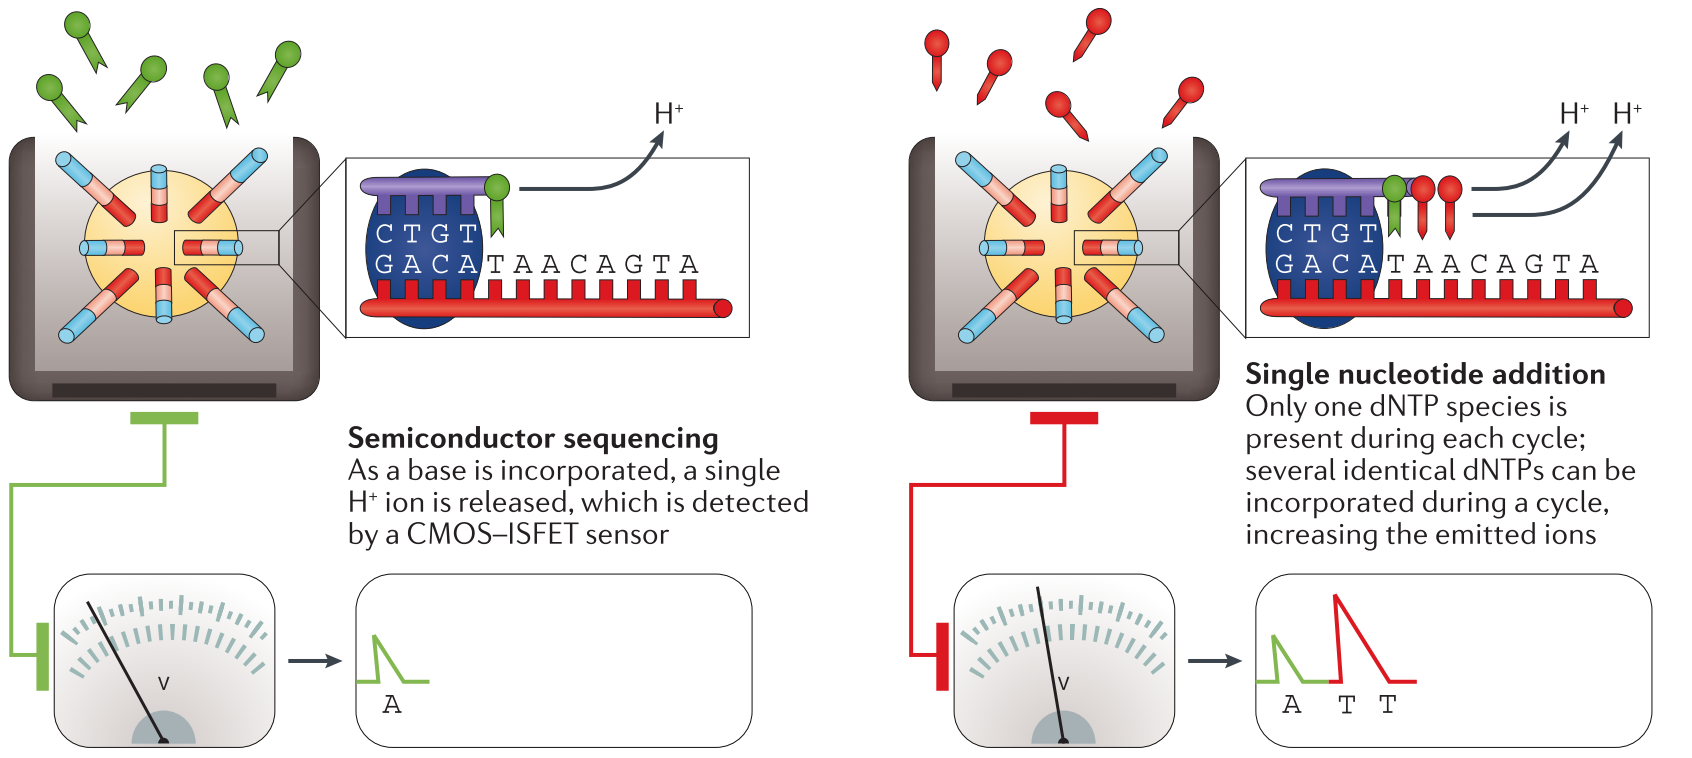
\includegraphics[scale=.26]{figure/SNA_seq_ionTorrent} 

}

\caption[Séquençage SNA tel qu'il est effectué par Ion Torrent]{\textbf{\emph{Séquençage SNA tel qu'il est effectué par
Ion Torrent} d'après {[}\protect\hyperlink{ref-Goodwin2016}{113}{]}} :
\textbf{a} : mise en présence du patron d'ADN à séquencer avec un mix
contenant un seul type de dNTP, si le dNTP est complémentaire au patron,
il se fixe et libère un proton permettant d'identifier la liaison.
\textbf{b} : dans le cas d'homopolymère, autant de protons sont relâchés
que de bases constituant l'homopolymère, le signal émis est donc plus
fort permettant d'identifier le nombre des dNTPs liés.}\label{fig:pictsnaSeq}
\end{figure}










\newpage

\begin{enumerate}
\def\labelenumi{\arabic{enumi}.}
\setcounter{enumi}{1}
\tightlist
\item
  \textbf{Séquençage par ligation} (SBL) (\textbf{Figure :
  }\ref{fig:pictsblSeq}) : Par définition, cette méthode est basée sur
  l'hybridation et la ligation de l'ADN à une sonde liée à un
  fluorophore {[}\protect\hyperlink{ref-Tomkinson2006}{115}{]}. Ce
  processus utilise les caractéristiques de la ligase, une enzyme qui a
  pour fonction de catalyser la liaison de deux brins d'ADN par des
  liaisons phosphodiester. La sonde est constituée d'une de ou deux
  bases connues, on parle alors de \emph{one-base-encoded probes} ou de
  \emph{two-bases-encoded probes} suivies d'une succession de bases
  ``dégénérées'' ou universelles, c'est à dire, de bases capables de
  s'apparier avec n'importe laquelle des quatre bases de l'ADN.
\end{enumerate}

\begin{figure}

{\centering 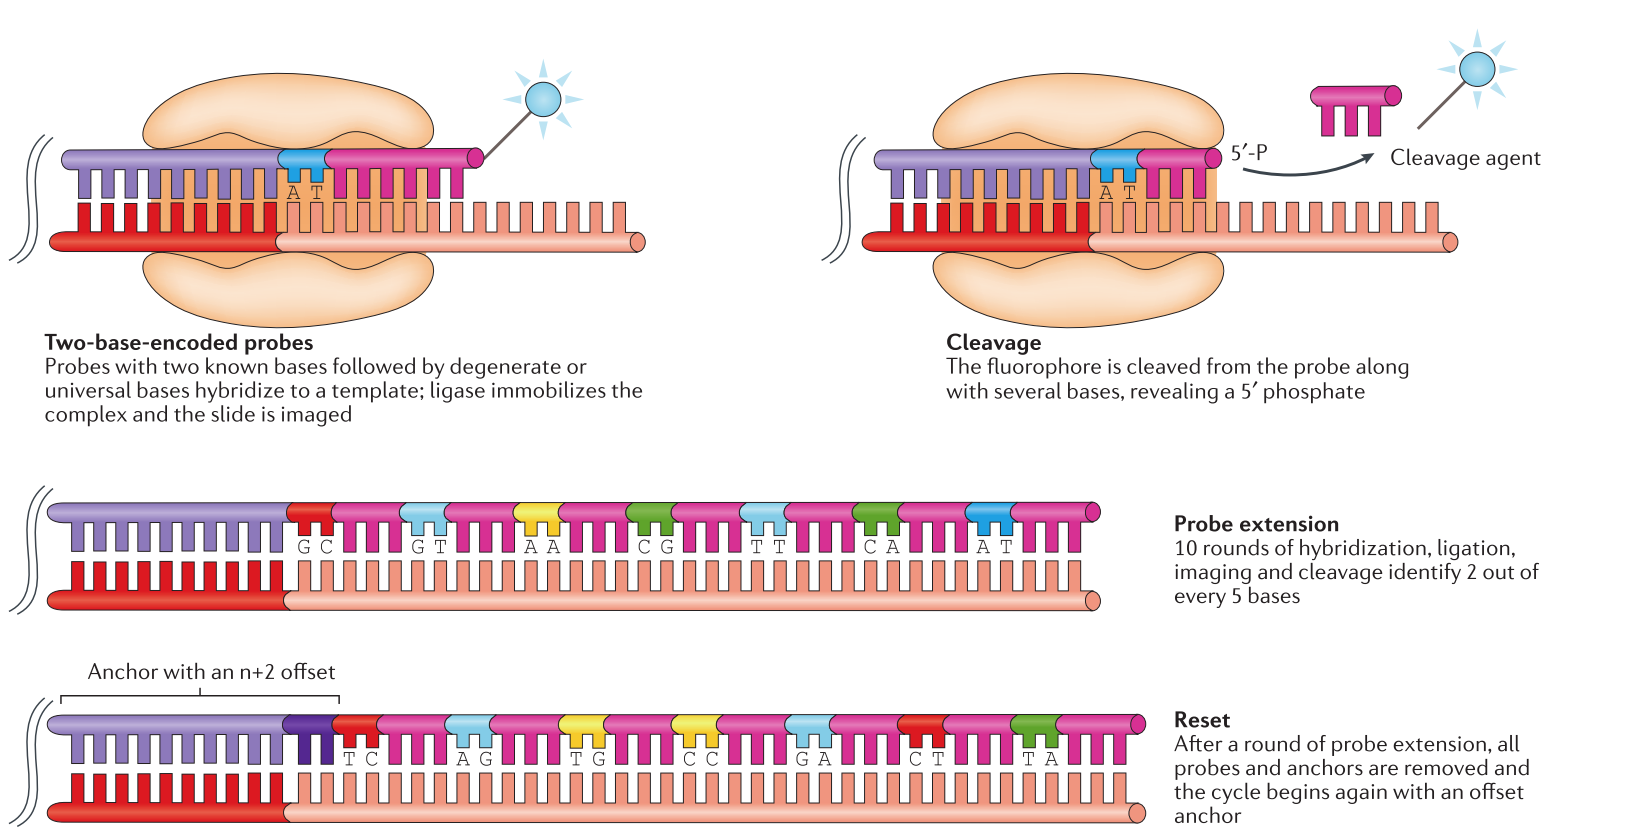
\includegraphics[scale=.26]{figure/SBL_seq_solid} 

}

\caption[Séquençage SBL tel qu'il est effectué par SOLiD]{\textbf{\emph{Séquençage SBL tel qu'il est effectué par
SOLiD} d'après {[}\protect\hyperlink{ref-Goodwin2016}{113}{]}} :
\textbf{a} : dans cette phase d'initialisation, un ensemble de sondes
composées de deux nucléotides connus suivis de bases dégénérées et de
bases universelles est reliée en 5' à un fluorophore. De fait qu'il n'y
ait que quatre fluorophores différents, un même fluorophore est utilisé
pour quatre combinaisons de dinucléotides parmi les seize possibles.
\textbf{b} : après avoir été hybridé grâce à une ligase, aux brin d'ADN
à séquencé, le fluorophore est identifié permettant ainsi de déduire
l'une des quatre combinaisons possibles à ce locus. \textbf{c} : le
fluorophore ainsi qu'une partie des bases non spécifiques sont clivés.
\textbf{d} : les étapes \textbf{b} et \textbf{c} sont ensuite répétées
10 fois permettant à chaque fois d'identifier de réduire la liste des
dinucléotides possibles au locus en question. \textbf{e} : les étapes
\textbf{b}, \textbf{c}, et \textbf{d} sont répétées sur le même brin
avec un décalage d'un nucléotide jusqu'à ce que chaque position ait été
séquencée deux fois. \textbf{f} : en recoupant les informations obtenues
à chaque itération du cycle, la séquence nucléotidique est reconstituée.}\label{fig:pictsblSeq}
\end{figure}




















\newpage  

\section{L'analyse bioinformatique des données de
NGS}\label{lanalyse-bioinformatique-des-donnees-de-ngs}

La stratégie consistant à séquencer en parallèle plusieurs millions de
\emph{reads} courts a engendré de nombreux et nouveaux défis
bioinformatiques dans l'analyse et l'interprétation des données de
séquençage et la recherche de variants dans le génome humain
{[}\protect\hyperlink{ref-Wold2007}{116},
\protect\hyperlink{ref-Yang2009}{117}{]}. Ces techniques ont été
appliquées dans différents contextes, notamment la métagénomique
{[}\protect\hyperlink{ref-Qin2010}{118}{]}, la détection de SNPs
{[}\protect\hyperlink{ref-VanTassell2008}{119}{]} et de variants
structuraux {[}\protect\hyperlink{ref-Alkan2010}{120},
\protect\hyperlink{ref-Medvedev2009}{121}{]} mais également dans des
études portant sur la méthylation de l'ADN
{[}\protect\hyperlink{ref-Taylor2007}{122}{]}, l'analyse de l'expression
des ARNs messagers {[}\protect\hyperlink{ref-Sultan2008}{123}{]}, dans
la génétique du cancer {[}\protect\hyperlink{ref-Guffanti2009}{124}{]}
et la médecine personnalisée
{[}\protect\hyperlink{ref-Auffray2009}{125}{]}. Cependant, pour
l'ensemble de ces applications, la grande quantité de données générées
par chaque analyse pose plusieurs défis informatiques
{[}\protect\hyperlink{ref-Horner2009}{126}{]}. En effet, les progrès
techniques des dernières décennies ont rendu possible le séquençage de
plusieurs millions des \emph{reads} d'ADN en un temps relativement court
et à coût raisonnable. Ainsi, l'émergence du séquençage haut débit et
notamment du WGS et du WES a permis de réunir une quantité jusqu'à
présent inégalée d'informations sur les variations génétiques, et sur
les gènes et leurs fonctions {[}\protect\hyperlink{ref-Mardis2008}{127},
\protect\hyperlink{ref-Bentley2006}{128}{]}. Cependant, de par leur
nature et leur quantité, l'acquisition de ces nouvelles données a
engendré de nouvelles problématiques qui freinent les biologistes dans
leurs recherches.

\subsection{Les données fournies par le
NGS}\label{les-donnees-fournies-par-le-ngs}

\subsubsection{\texorpdfstring{Un \emph{read}, c'est quoi
?}{Un read, c'est quoi ?}}\label{un-read-cest-quoi}

Après la phase d'amplification, chaque clone est analysé, puis la
séquence composant chacun de ce clone est déterminée. La taille de cette
séquence varie en fonction des plateformes de séquençage mais est
généralement comprise entre 40 et 300 pb pour le NGS (\textbf{Figure :
}\ref{fig:pictreadPerRun}). Depuis quelques années, un nouveau type de
\emph{read} est apparu, le \emph{read} \emph{paired-end}. Contrairement
au \emph{reads} classiques (\emph{single-end}), les deux extrémités (les
\emph{ends}) du fragment d'ADN sont désormais séquencées. La distance
approximative séparant les deux extrémités du \emph{read} étant connue,
cela permet aux aligneurs d'utiliser cette information afin d'améliorer
leur précision, notamment dans les zones répétées
{[}\protect\hyperlink{ref-Li2008}{129}{]}. En plus de SNP, ce format
permet de mettre en évidence des variants structuraux
{[}\protect\hyperlink{ref-Korbel2009}{130}{]}.

\newpage

\subsubsection{Le format FASTQ}\label{fastq}

Le format FASTQ (\textbf{Figure : }\ref{fig:pictfastqformat}) est
actuellement le format de données le plus couramment utilisé dans le
cadre du séquençage haut-débit. Sa création est cependant antérieure à
l'émergence du NGS puisqu'il fut inventé à la fin du
XX\textsuperscript{ième} par Jim Mullikin au
\href{https://fr.wikipedia.org/wiki/Wellcome_Trust_Sanger_Institute}{Wellcome
Trust Sanger Institute} alors que le séquençage commençait à prendre de
l'ampleur grâce à des projets tels que le
\href{https://fr.wikipedia.org/wiki/Projet_G\%C3\%A9nome_Humain}{Projet
Génome Humain}. La quantité de données générées par ces programmes a
nécessité une analyse automatisée. C'est ainsi que chaque base séquencée
s'est vu associer un score de qualité appelé \emph{Phred-score}. Chaque
séquence générait ainsi deux fichiers, un fichier FASTA contenant les
séquences et un fichier QUAL contenant les scores \emph{Phred} associés
à chaque base du fichier FASTA
{[}\protect\hyperlink{ref-Cock2009}{131}{]}. Plus tard, afin de n'avoir
à manipuler qu'un seul fichier, les fichiers FASTA et QUAL furent
fusionnés en ce que l'on appelle désormais le fichier FASTQ. Ce format
est aujourd'hui le plus utilisé par les différents séquenceurs. On peut
cependant noter certaines différences dans les formats FASTQ provenant
des différentes plateformes, puisqu'à l'époque, aucune spécification
officielle n'avait été donnée
{[}\protect\hyperlink{ref-Cock2009}{131}{]}.

\begin{figure}

{\centering 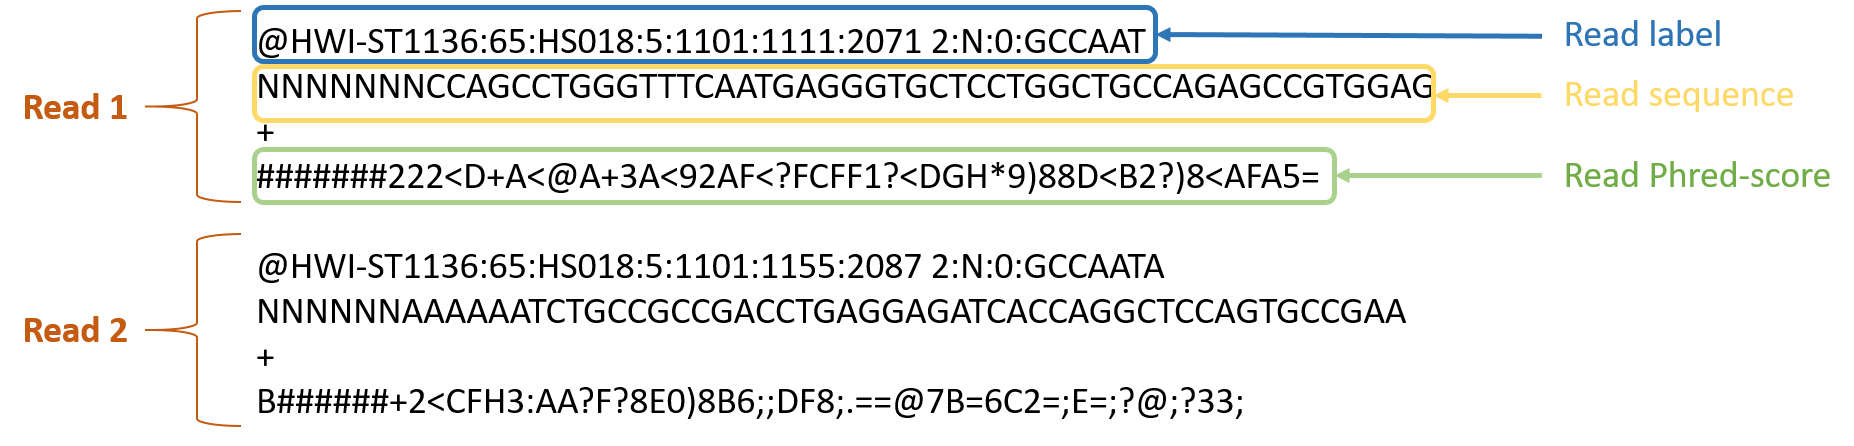
\includegraphics[scale=.36]{figure/fastq} 

}

\caption[Présentation d'un fichier FASTQ]{\textbf{\emph{Présentation d'un fichier FASTQ}} :
Chaque \emph{read} présent au sein d'un fichier FASTQ est composé d'un
label, d'une séquence et d'un score de qualité associé à chaque
nucléotide de la séquence.}\label{fig:pictfastqformat}
\end{figure}






\newpage

\hypertarget{lalignement}{\subsection{L'alignement}\label{lalignement}}

L'alignement constitue la première étape de l'analyse des données de NGS
lorsqu'un génome de référence est disponible. L'objectif de l'alignement
est de déterminer la position correcte de chacun des \emph{reads}
séquencés le long du génome de référence. Cette référence est souvent
construite à partir des données de séquençage de plusieurs donneurs et
ne représente donc pas la séquence d'un individu en particulier mais est
censée représenter la séquence consensus d'une espèce donnée. Par
exemple, la séquence de référence humaine GRCh37 (\emph{Genome Reference
Consortium human build 37}) a été créée à partir de treize volontaires
anonymes New-Yorkais. Dès lors, cette référence servira de patron aux
aligneurs afin qu'ils replacent correctement les différents \emph{reads}
des individus séquencés. Cette étape peut être comparée à la
reconstruction d'un puzzle dans lequel les \emph{reads} seraient les
pièces et le génome de référence le modèle (\textbf{Figure :
}\ref{fig:picdnamapping}). Elle constitue probablement l'étape la plus
importante de l'analyse des données issues du séquençage haut débit
{[}\protect\hyperlink{ref-Flicek2009}{132}{]} car elle est la base sur
laquelle repose l'ensemble des étapes effectuées en aval, notamment
l'appel des variants {[}\protect\hyperlink{ref-Nielsen2011}{133}{]}.
Cependant, l'étape d'alignement est sujette à de nombreuses erreurs dont
certaines proviennent directement des erreurs survenues lors de l'étape
de séquençage. D'autres, sont dues aux caractéristiques des régions
séquencées comme par exemple les séquences répétées
{[}\protect\hyperlink{ref-Langmead2012}{134}{]} qui pourront entraîner
l'alignement d'un même \emph{read} à plusieurs régions du génome
{[}\protect\hyperlink{ref-Treangen2013}{135}{]}. De nombreux aligneurs
ont émergé afin de répondre au mieux à cette problématique tel que
Bowtie {[}\protect\hyperlink{ref-Langmead2009}{136}{]}, Bowtie2
{[}\protect\hyperlink{ref-Langmead2012}{134}{]}, BWA, NovoAlign, MAGIC
{[}\protect\hyperlink{ref-Su2014}{137}{]}. De nombreuses études ont
cependant montré de grandes différences entre ces aligneurs, au niveau
du temps de calcul, de leur coût en mémoire et de leur taux d'erreur
{[}\protect\hyperlink{ref-Ruffalo2011}{138}--\protect\hyperlink{ref-Bao2011}{140}{]}.

\newpage

\begin{figure}

{\centering \includegraphics[scale=0.35]{figure/dna_mapping} 

}

\caption[Représentation schématique de l'alignement de reads paired-end]{\textbf{\emph{Représentation schématique de
l'alignement de reads paired-end}} : \textbf{A} : représentation du
génome de référence ainsi que de \emph{reads paired-end} avant l'étape
d'alignement. Les \emph{reads paired-end} sont composés d'une extrémité
\emph{forward} (en vert) complémentaire du brin sens du génome de
référence et d'une extrémité réverse (en jaune), complémentaire du brin
anti-sens du génome de référence. Chacune de ces extrémités est séparée
par un insert de taille connue mais de séquence inconnu. \textbf{B} :
après l'étape d'alignement, chaque \emph{read} est repositioné sur la
région du génome avec laquelle il présente la plus grande homologie de
séquence. Le nombre de \emph{reads} différents recouvrant une même
position du génome de référence est appellé couverture.}\label{fig:picdnamapping}
\end{figure}














\newpage

\hypertarget{varcall}{\subsection{L'appel des variants}\label{varcall}}

L'appel des variants, ou \emph{variant calling}, fait référence à
l'ensemble des méthodes permettant d'identifier des SNVs ou des indels à
partir des résultats de l'alignement. Cette étape est souvent
différenciée de l'alignement, cependant, les résultats de l'appel étant
extrêmement dépendants de l'alignement, il est conseillé d'effectuer son
appel en tenant compte de l'aligneur choisi
{[}\protect\hyperlink{ref-Nielsen2011}{133},
\protect\hyperlink{ref-DePristo2011}{141},
\protect\hyperlink{ref-Lunter2011}{142}{]}. On appellera variant toute
différence de séquence observée entre un individu et la séquence de
référence utilisée. Pour reprendre la comparaison avec la construction
d'un puzzle, cette étape consiste à détecter quelles sont les pièces qui
présentent des différences avec le modèle.

\begin{figure}

{\centering \includegraphics[scale=0.33]{figure/var_call_exemple} 

}

\caption[Illustration schématique du processus d'appel des variants]{\textbf{\emph{Illustration schématique du
processus d'appel des variants}} : Pour chaque position couverte,le
pourcentage de \emph{read} portant un allèle variant est analysé.
Lorsque l'on est ptoche des 100 pourcent l'appel est homozygote pour le
variant, lorsque l'on est proche des 50 pourcent l'appel des
hétérozygote. Lorsqu'à une position donnée, peu de \emph{reads} portent
un variant, la cause est souvent une erreur de séquençage.}\label{fig:picvarcallprocess}
\end{figure}









De nombreux logiciels d'appels des variants, ou \emph{caller}, basés sur
des algorithmes différents ont émergé ces dernières années pour répondre
à cette problématique. Parmi les plus connus on note SAMtools
{[}\protect\hyperlink{ref-Li2009}{143}{]}, Genome Analysis Tool Kit -
HaplotypeCaller (GATK-HC)
{[}\protect\hyperlink{ref-McKenna2010}{144}{]}, Freebayes, SOAPindel et
TVC. Les quatre premiers cités, peuvent être utilisés pour analyser des
données provenant de tout type de plateforme de séquençage contrairement
à TVC qui a été développé spécifiquement pour les données provenant de
Ion Proton. Les données issues de NGS peuvent présenter un taux d'erreur
important. Ce taux d'erreur est multifactoriel et inclut notamment les
erreurs de l'alignement. L'un des éléments clef à prendre en compte pour
pouvoir effectuer un appel de qualité est la couverture de la position
appelée {[}\protect\hyperlink{ref-Sims2014}{108}{]}. Cependant, malgré
la prise en compte de cet élément, l'appel de variants reste un
processus difficile souvent lié à plusieurs erreurs. Plusieurs de ces
erreurs sont même directement liées à la plateforme de séquençage
utilisée en amont, et les différents logiciels ne présentent pas les
mêmes performances en fonction de ces différentes plateformes
{[}\protect\hyperlink{ref-Hwang2015}{145}{]}. C'est pourquoi, il
convient d'adapter le logiciel d'appel en fonction de la plateforme de
séquençage utilisée préalablement. Les erreurs d'appel sont généralement
classées en trois catégories et certains aligneurs auront tendance à
être plus sujets à l'un de ces types d'erreur qu'à l'autre
(\textbf{Figure : }\ref{fig:pictsnperror}) :

\begin{enumerate}
\def\labelenumi{\arabic{enumi}.}
\item
  Oubli de l'allèle de référence (\textbf{IR}, \emph{ignore the
  reference allele}) : représente un variant appelé homozygote
  correspondant en réalité à un variant hétérozygote composé de l'allèle
  de référence et d'un allèle variant.
\item
  Ajout de l'allèle de référence (\textbf{AR}, \emph{adding the
  reference allele}) : représente un variant appelé hétérozygote composé
  de l'allèle de référence et d'un allèle variant correspondant en
  réalité à un variant homozygote composé de deux allèles variants.
\item
  Autres : incluent l'ensemble des autres types d'appel erronés
  indépendamment de l'allèle de référence.
\end{enumerate}

\begin{figure}

{\centering 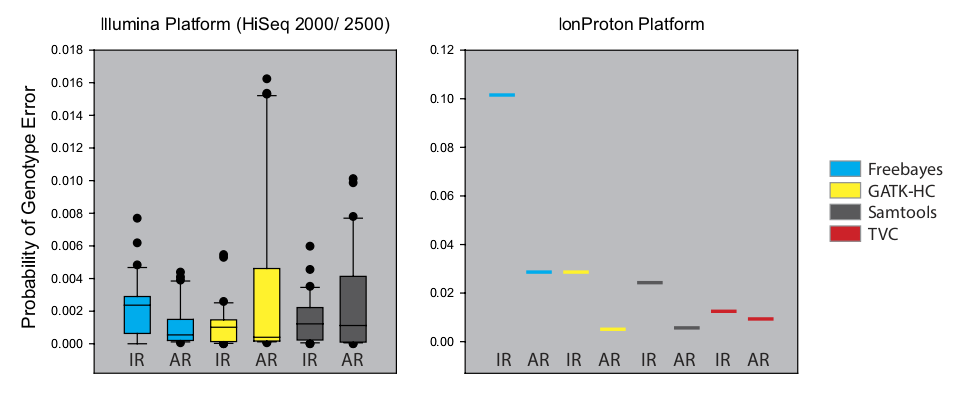
\includegraphics[scale=.37]{figure/snp_error_type} 

}

\caption[Représentation des erreurs d'appel de type IR et AR en fonction de la plateforme de séquençage et du logiciel d'appel.]{\textbf{\emph{Représentation des erreurs d'appel de
type IR et AR en fonction de la plateforme de séquençage et du logiciel
d'appel.} d'après {[}\protect\hyperlink{ref-Hwang2015}{145}{]}} : Pour
la plateforme Illumina, on peut voir que Freebayes favorise les appels
variant-homozygote tandis que GATK-HC et Samtools favorisent les appels
hétérozygotes. Pour la plateforme Ion Proton, les quatre logiciels
entraînent des erreurs de type IR}\label{fig:pictsnperror}
\end{figure}









De même que pour l'aligneur, le choix du logiciel d'appel est crucial
car il existe de nombreuses différences dans les variants appelés par
différents logiciels se basant sur les mêmes données brutes
{[}\protect\hyperlink{ref-Baes2014}{146}--\protect\hyperlink{ref-Rosenfeld2012}{148}{]}.
En effet, en 2013, une étude comparant les résultats de 5 \emph{callers}
montraient que seulement 57,4\% des variants étaient appelés par les 5
\emph{callers} et que 80,7\% des variants étaient appelés par au moins 3
d'entre eux. Ce taux chutait drastiquement pour les indels puisque la
concordance était cette fois seulement de 26,8\% pour les indels non
retrouvés par les 3 \emph{callers}
{[}\protect\hyperlink{ref-ORawe2013}{147}{]}. Ces résultats sont
cependant à pondérer avec une étude de 2015 comparant 4 \emph{callers}
et montrant que 91,7\% des SNVs séquencés sur une plateforme Illumina
étaient appelés par 3 \emph{callers}, cependant, pour les variants
séquencés sur Ion Proton, seulement 27,3\% des variants étaient appelés
par au moins 3 \emph{callers} et 57,4\% des variants n'étaient appelés
que par un seul des \emph{callers}
{[}\protect\hyperlink{ref-Hwang2015}{145}{]}.

\newpage

\subsection{L'annotation des variants}\label{lannotation-des-variants}

Traditionnellement, les scientifiques et les laboratoires dans lesquels
ils travaillaient développaient leur expertise dans un nombre de
pathologies et de gènes associés limité. L'émergence du NGS est en train
de remettre en cause cette pratique car la totalité de l'exome ou du
génome peut permettre de couvrir tous les gènes en une seule et même
analyse. De nombreux praticiens maintiennent cependant une
spécialisation pour certains groupes de pathologies qui est précieuse
pour l'analyse des données et l'obtention d'un diagnostic. En effet il
est courant de retrouver entre 20.000 et 25.000 variants différents par
exome {[}\protect\hyperlink{ref-Gonzaga-Jauregui2012}{149}{]}. Afin de
pouvoir lier un variant à une pathologie, il est indispensable d'annoter
cet ensemble de variants, c'est à dire d'associer à ces variants
l'ensemble des informations qui les caractérisent afin de pouvoir les
replacer dans leur contexte biologique. Ces informations serviront
ensuite d'indicateur afin de filtrer ou de prioriser un variant. Cette
dernière étape de l'analyse est, elle aussi, cruciale puisqu'elle permet
de réduire le nombre de variants à considérer. On peut généralement
distinguer deux niveaux d'annotations d'un variant (\textbf{Figure :}
\ref{fig:pictannot}) :

\begin{enumerate}
\def\labelenumi{\arabic{enumi}.}
\tightlist
\item
  \textbf{Au niveau du variant} : Ce niveau d'annotation regroupe
  l'ensemble des informations \textbf{spécifiques} à un variant

  \begin{enumerate}
  \def\labelenumii{\alph{enumii}.}
  \item
    \textbf{Informations issues des résultats du séquençage} : la
    couverture du variant ainsi que la qualité qui lui est associée
    peuvent permettre de considérer un variant comme étant fiable ou
    non. Le génotype associé à ce variant est également une information
    importante.
  \item
    \textbf{La fréquence du variant dans la population générale} :
    l'émergence du séquençage haut-débit a permis de gros consortiums
    tels que ESP6500 (\href{http://evs.gs.washington.edu/EVS/}{Exome
    Variant Server, NHLBI GO Exome Sequencing Project (ESP), Seattle,
    WA}), 1KG
    {[}\protect\hyperlink{ref-1000GenomesProjectConsortium2015}{150}{]}.
    Ces consortiums ont pu mettre à disposition du public des données de
    séquençage exomique de 6503 individus pour ESP et de 2504 pour la
    phase 3 du 1000Genomes. On peut également noter l'\emph{Exome
    Aggregate Consortium} (ExAC)
    {[}\protect\hyperlink{ref-Lek2016}{151}{]} qui n'a effectué aucun
    séquençage mais qui a regroupé les données de plusieurs gros jeux
    (notamment 1000Genome et ESP) afin de leur appliquer la même analyse
    bioinformatique harmonisant ainsi les données provenant de 60.706
    individus non apparentés. Cette masse d'information permet de se
    faire une idée de la fréquence d'un variant dans la population
    générale et même au sein de sous-populations humaines. On considère
    qu'un variant fréquent ne peut pas être délétère, sinon il aurait
    été contre-sélectionné au cours de l'évolution.
  \item
    \textbf{Son impact sur le transcrit} : Dans la plupart des analyses
    phénotype-génotype, les chercheurs se limitent aux variants
    chevauchant des transcrits codants pour une protéine. Il est donc
    important de savoir l'impact d'un variant sur ce transcrit, c'est à
    dire si le variant va causer une mutation synonyme, un faux-sens ou
    une mutation tronquante. Des logiciels tels que \emph{Variant Effect
    Predictor} (VEP) {[}\protect\hyperlink{ref-McLaren2016}{152}{]},
    SnpEff {[}\protect\hyperlink{ref-Cingolani2012}{153}{]} ou encore
    ANNOVAR {[}\protect\hyperlink{ref-Wang2010}{154}{]} vont prédire
    l'impact qu'aura un variant sur les différents transcrits qu'il
    chevauche. D'autres logiciels tel que SIFT
    {[}\protect\hyperlink{ref-Kumar2009}{155}{]}, PROVEAN
    {[}\protect\hyperlink{ref-Choi2012}{156}{]}, Polyphen2, ou encore
    CADD vont, eux, chercher à prédire la pathogénicité de ce variant,
    c'est à dire la probabilité que ce variant soit délétère pour la
    fonction de la protéine. Bien que cette information soit importante,
    elle est à pondérer, étant donné le peu de concordance qu'il existe
    entre les prédictions de ces différents logiciels (\textbf{Figure :}
    \ref{fig:pictvennpred}).
  \end{enumerate}
\end{enumerate}

\begin{figure}

{\centering 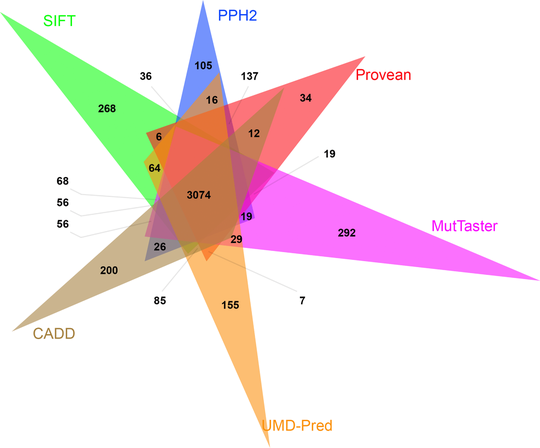
\includegraphics[scale=.7]{figure/venn_Diag_patho_pred} 

}

\caption[Diagramme de Venn des prédictions de pathogénicité de variants de six logiciels]{\textbf{\emph{Diagramme de Venn des prédictions de
pathogénicité de variants de six logiciels} d'après
{[}\protect\hyperlink{ref-Salgado2016}{157}{]}} : Les six logiciels
utilisés sont : CADD {[}\protect\hyperlink{ref-Kircher2014}{158}{]}
(marron), SIFT {[}\protect\hyperlink{ref-Kumar2009}{155}{]} (vert),
PolyPhen2 {[}\protect\hyperlink{ref-Adzhubei2010}{159}{]} (bleu),
Provean {[}\protect\hyperlink{ref-Choi2012}{156}{]} (rouge)
MutationTaster {[}\protect\hyperlink{ref-Schwarz2010}{160}{]} (violet)
et UMD-Predictor {[}\protect\hyperlink{ref-Salgado2016a}{161}{]}
(orange).}\label{fig:pictvennpred}
\end{figure}












\newpage

\begin{enumerate}
\def\labelenumi{\arabic{enumi}.}
\setcounter{enumi}{1}
\tightlist
\item
  \textbf{Au niveau du gène (ou transcrit)} : L'annotation au niveau du
  gène consiste à récupérer l'ensemble des informations disponibles non
  plus sur le variant uniquement mais sur le ou les gènes qu'il impacte.
  Ce ``dézoom'' permet d'ajouter des informations complémentaires
  particulièrement utiles notamment lorsque peu d'informations sont
  disponibles sur le variant lui-même. En pratique, la plupart des
  variants connus pour impliquer une pathologie sont des variants
  privés, c'est à dire spécifiques à une famille ou à un individu,
  limitant ainsi la quantité d'information disponible sur ce variant.
  Élargir l'annotation au niveau des gènes impactés par des variants
  permet d'augmenter considérablement la quantité d'information
  disponible et permet donc d'améliorer la capacité des algorithmes à
  filtrer et / ou prioriser les variants rendant donc les analyses plus
  efficaces. On peut relever certains logiciels tel que le \emph{Protein
  ANalysis THrough Evolutionary Relationships} (PANTHER)
  {[}\protect\hyperlink{ref-Mi2017}{162}{]} qui permettent par exemple
  de classer une liste de gènes en fonction de leurs fonctions
  moléculaires, des processus biologiques et des voies de signalisation
  dans lesquelles ils sont impliqués. On peut également noter \emph{the
  Human Phenotype Ontology project} (HPO)
  {[}\protect\hyperlink{ref-Kohler2014}{163}{]} qui fournit un
  vocabulaire standardisé pour les anomalies phénotypiques observées
  dans les pathologies humaines et une liste de gènes connus pour être
  associés à ces phénotypes. Plus récemment, on a pu voir émerger des
  ``scores mutationnels'' tel que RVIS
  {[}\protect\hyperlink{ref-Petrovski2013}{164}{]} ou encore le pLI
  {[}\protect\hyperlink{ref-Lek2016}{151}{]}. En se basant sur les bases
  de données telle que ESP ou encore ExAC, ces scores permettent de
  classer les gènes en fonction de leur tolérance (ou intolérance) aux
  variations avec l'idée sous-jacente que ``les gènes impliqués dans des
  pathologies à transmission mendéliennes'' devraient être moins
  tolérants aux variations que les autres.
\end{enumerate}

\begin{figure}

{\centering \includegraphics[scale=.27]{figure/annotation_process} 

}

\caption[Représentation simplifié du processus d'annotation]{\textbf{\emph{Représentation simplifié du processus
d'annotation}} : On peut observer deux niveaux d'annotation, le premier
est l'annotation des variants consistant à ajouter un maximum
d'information sur un variant spécifique (sa fréquence, son
impact\ldots{}). La deuxième est au niveau du gène, consistant à
récupérer pour les gènes impactés par les variants l'ensemble des
informations disponibles tel que les processus biologiques dans lesquels
il est impliqué, ou encore son expression tissulaire.}\label{fig:pictannot}
\end{figure}










\newpage

\subsection{Le filtrage des variants}\label{le-filtrage-des-variants}

L'étape de filtrage a pour principal objectif de restreindre le nombre
de variants obtenu à l'issus de l'appel afin que ceux-ci puissent être
analysés par un être humain. Pour cela il utilise l'ensemble des
information obtenues lors de l'étape d'annotation afin de filtrer les
variants ayant le moins de risque d'être responsables du phénotype.
Communément, les variant ayant une forte fréquence dans les bases de
données ExAC, ESP6500 ou encore 1KG sont filtrés avec l'idée
sous-jacente que des variants observés fréquement dans la population ne
peuvent être responsables de phénotypes sévères.

Comme nous l'avons vu, le développement d'outils permettant l'analyse et
le filtrage des données NGS est extrêmement important puisqu'il permet
aux biologistes de faire face à la masse de données générée par le
séquençage haut-débit l'aidant ainsi dans ses prises de décisions. Il
est à noter que la plupart de ces données filtrées sont extrêmement
dépendantes du jeu de transcrits utilisés. Les prédictions seront donc
différentes si l'on se base sur les transcrits RefSeq, Ensembl ou UCSC
{[}\protect\hyperlink{ref-McCarthy2014}{165}{]} bien que les transcrits
du \emph{Consensus Coding Sequence project} (CCDS) soient bien
représentés par ces trois listes
{[}\protect\hyperlink{ref-Pruitt2009}{167}{]}. De même, pour une même
liste de gène, de nombreuses différences seront observées en fonction du
ou des logiciels de prédiction utilisés
{[}\protect\hyperlink{ref-Salgado2016}{157},
\protect\hyperlink{ref-McCarthy2014}{165}{]}.

\newpage

\begin{figure}

{\centering \includegraphics[scale=.3]{figure/filtering_process} 

}

\caption[Représentation simplifié du processus de filtrage des variants]{\textbf{\emph{Représentation simplifié du processus de
filtrage des variants}} : L'ensemble des annotations ajoutées lors de
l'étape précédente servent alors de support pour filtrer (ou non) les
variants. Il est par exemple commun de filtrer les variants ayant une
forte fréquence dans la population générale ou encore ceux ayant un
impact faible sur la protéine. De même dans le cas d'étude sur des
pathologies ayant un mode de transmission recessif, les variants
hétérozygotes pourront être également filtrés.}\label{fig:pictfilter}
\end{figure}










\newpage

\subsection{Conclusion NGS}\label{conclusion-ngs}

En moins de 10 ans, les technologies NGS sont passées du séquençage de
panels de gènes (environ 100 Mb pour le Roche GS FLX system) au
séquençage de génomes entiers (environs 1500 GB pour l'Illumina Hiseq
4000) et d'une utilisation exclusive à la recherche à l'analyse en
routine dans un cadre de diagnostics cliniques. Le nombre croissant
d'études utilisant le WGS ou le WES démontre le pouvoir de ces approches
dans des analyses phénotype-génotype impliquant des pathologies à
transmission mendélienne. De plus, la diminution constante des coûts par
génomes / exomes séquencés laisse supposer que ces technologies
deviendront d'ici peut le fer de lance de la génétique clinique moderne.
Cependant, la quantité de données produites crée de nouvelles
problématiques pour les généticiens qui se retrouvent désormais face au
``déluge de données génétiques''
{[}\protect\hyperlink{ref-Schatz2013}{168}{]}. Le succès d'une étude
n'étant plus lié aux capacités de séquençage mais aux compétences dans
l'analyse et l'interprétation des données produites à chaque étape
(\textbf{Figure :} \ref{fig:pictrecapngssteps}). Bien que de nombreux
efforts soient faits pour palier la contrainte instaurée par les
\emph{reads} courts dans le cadre d'analyse génomique, les solutions
informatiques et bioinformatiques proposées jusqu'à présent restent en
dessous des besoins créés par NGS
{[}\protect\hyperlink{ref-McPherson2009}{169}{]}. Cette masse de données
produite, à l'origine du succès du séquençage haut-débit dans le domaine
de la génomique et de la post-génomique, se trouve désormais être un
frein à la compréhension et à l'interprétation des réseaux de gènes et
leurs implications dans des pathologies. La limitation de cette
technologie n'est donc plus le séquençage d'un, de plusieurs, ou de
l'ensemble des gènes, mais plutôt l'analyse et l'interprétation des
données générées. Le processus allant de l'extraction de l'ADN à
l'identification d'un variant responsable d'une pathologie comprend de
nombreuses étapes apportant avec elles leurs lots d'erreurs. Bien que
dans chacune de ces phases, de nombreux acteurs soient en concurrence et
cherchent à atteindre une solution idéale, celle-ci n'a toujours pas été
trouvée et la prolifération des logiciels et algorithmes d'analyses,
bien que nécessaire, peut également parfois augmenter la confusion.

Malgré les dizaines de milliers d'exomes et de génomes ayant été jusqu'à
présent étudiés, notre compréhension des mécanismes moléculaires qui
sous-tendent la variété génomique humaine reste limitée, et ce
particulièrement dans le contexte de l'analyse de pathologies
génétiques. En effet, à l'heure actuelle, plus de 3700 pathologies à
transmission mendélienne ont été caractérisées mais un nombre similaire
a toujours une cause inconnue
{[}\protect\hyperlink{ref-Amberger2011}{170}{]}. L'élucidation de ces
mystères passera probablement par une harmonisation des méthodes de
production des données ainsi que par l'amélioration des techniques
d'analyses.

\newpage 

\begin{figure}

{\centering \includegraphics[scale=.3]{figure/bioinformatic_steps} 

}

\caption[Récapitulatif des différentes étapes du séquençage NGS dans le cadre d'une étude phénotype-génotype]{\textbf{\emph{Récapitulatif des différentes
étapes du séquençage NGS dans le cadre d'une étude phénotype-génotype}}
: L'ADN est d'abord extrait, puis fragmenté. Les fragments sont liés à
des adaptateurs puis amplifiés. Ces amplifiats sont alors isolés et
soumis à une amplification clonale (schéma de l'amplification clonale
est adapté d'après {[}\protect\hyperlink{ref-Goodwin2016}{113}{]}).
Chacun des clones est ensuite séquencé. Les \emph{reads} générés à
l'issu du séquençage sont stockés dans des fichiers FASTQ qui serviront
de base pour l'étape d'alignement à la suite de laquelle, les variants
et leur génotype seront appelés puis annotés. Ces annotations serviront
ensuite pour filtrer les variants jugés non pertinent dans le cadre de
l'étude, les variants / gènes restant seront ensuite prioriser de sorte
à identifier le/les variant(s) responsable(s) du phénotype.}\label{fig:pictrecapngssteps}
\end{figure}















\chapter{Mise en place d'une stratégie pour l'analyse des données
exomiques -- application en recherche
clinique}\label{mise-en-place-dune-strategie-pour-lanalyse-des-donnees-exomiques-application-en-recherche-clinique}

\newpage

En 2011, les bases moléculaires d'environ 3700 pathologies à
transmission mendélienne avaient été élucidées. Cependant, pour une
quantité équivalente de pathologies Mendéliennes (ou suspectées de
l'être) cette cause reste un mystère
{[}\protect\hyperlink{ref-Amberger2011}{170}{]}. Avec plusieurs
centaines de pathologies caractérisées depuis 2010
{[}\protect\hyperlink{ref-Ng}{171}{]}, les séquençages WGS et WES ont,
depuis leur émergence, révolutionné les méthodes de recherche dans le
cadre d'étude phénotype-génotype en permettant de manière rapide et à
moindre coût le séquençage de la quasi-totalité des gènes humains. Dès
lors, le défi de ces analyses n'est plus le séquençage de l'ADN mais
l'interprétation des données massives produites. En effet, l'un des plus
grands challenges des analyses phénotype-génotype réalisées par WES
réside dans l'analyse de l'importante quantité de variants portée par
chaque individu s'élevant à plusieurs dizaines de milliers lorsque l'on
compare avec le génome de référence. Même après avoir retiré les
variants retrouvés fréquemment dans la population générale, des méthodes
additionnelles sont nécessaires pour prédire, parmi les variants
restant, lesquels induisent des conséquences fonctionnelles sérieuses
afin de les prioriser {[}\protect\hyperlink{ref-Pelak2010}{172}{]}. De
nombreux logiciels tel que Variant Effect Predictor
{[}\protect\hyperlink{ref-McLaren2016}{152}{]}, SnpEff
{[}\protect\hyperlink{ref-Cingolani2012}{153}{]} ou encore ANNOVAR
{[}\protect\hyperlink{ref-Wang2010}{154}{]} permettent d'identifier
quels sont les variants qui ont un effet tronquant sur la protéine.
Cependant, avec en moyenne 165 variants homozygotes ayant un effet
tronquant retrouvés dans chaque exome
{[}\protect\hyperlink{ref-Pelak2010}{172}{]} ces méthodes, bien
qu'efficaces sont souvent insuffisantes.

D'autres logiciels tel que Exomiser
{[}\protect\hyperlink{ref-Robinson2014}{173}{]} vont, à partir d'une
liste de variants déjà appelés, effectuer les étapes d'annotation, de
filtrage et de priorisation. Malgré l'efficacité de ces logiciels, aucun
d'entre eux ne couvre l'ensemble des étapes allant de l'alignement des
\emph{reads} à la priorisation des variants, la plupart ayant pour point
de départ une liste de variants appelés en amont. Ils ne contrôlent donc
en aucune manière les étapes d'alignement et d'appel des variants. Or,
comme il a été dit plus tôt, ces deux étapes constituent la base de
l'analyse.

Ce chapitre décrit à la fois la constitution d'un pipeline d'analyse des
données de séquençage exomique recouvrant l'ensemble des étapes allant
de l'alignement des séquences à la priorisation des variants ainsi que
son utilisation dans le cadre de la recherche de mutations entrainant
différents phénotypes d'infertilité d'une part au sein de cas familiaux
et, d'autre part, au sein d'une large cohorte d'individus non apparentés
présentant tous un phénotype MMAF.

\newpage

\section{Méthode : Description du
pipeline}\label{methode-description-du-pipeline}

\subsection{\texorpdfstring{L'alignement des
\emph{reads}}{L'alignement des reads}}\label{lalignement-des-reads}

Comme expliqué plus tôt, l'étape d'alignement a pour objectif de
repositionner l'ensemble des \emph{reads} d'un individu le long d'un
génome de référence. Cette étape peut ainsi être comparée à la
reconstruction d'un puzzle dans lequel chaque \emph{read} peut être
assimilé à l'une des pièces tandis que le génome de référence serait ici
le modèle (\textbf{Figure : }\ref{fig:picdnamapping}).

L'ensemble de nos exomes ayant été réalisé en \emph{paired-end}, les
deux extrémités de chaque fragment sont séquencées. Chaque \emph{end}
d'un même \emph{read} peut donc être considérée comme un \emph{read} à
part entière qui est aligné \textbf{indépendamment} le long du génome de
référence ; l'information fournie par le \emph{paired-end} n'étant
utilisée qu'\emph{a posteriori} en tant que critère qualité. Au sein de
notre pipeline, cette étape est effectuée par le logiciel MAGIC
{[}\protect\hyperlink{ref-Su2014}{137}{]}, qui, dans le cadre de nos
études, s'est basé sur la version hg19 / GHRC37 du génome de référence.
Suite à cet alignement, plusieurs critères sont observés afin de filtrer
les \emph{reads} présentant une faible qualité d'alignement.

Ainsi, le premier de ces filtres consiste à tout d'abord filtrer
l'ensemble des \emph{reads} dupliqués, c'est à dire les \emph{reads}
ayant des séquences parfaitement identiques, ceux-ci étant souvent le
résultat d'un excès d'amplification au moment des PCRs effectuées en
amont. De la même manière, afin d'éviter toute ambiguïté au moment de
l'interprétation des résultats, l'ensemble des \emph{reads} s'étant
aligné sur plusieurs régions du génome est aussi filtré. Une fois cela
fait, nous vérifions la ``compatibilité'' des deux \emph{ends} composant
chacun des \emph{reads} restant. Un \emph{read} est dit compatible
lorsque les deux \emph{ends} qui le composent s'alignent face à face
(une sur le brin sens du génome de référence et l'autre sur le brin
anti-sens) et couvrent une zone ne faisant pas plus de 3 fois la taille
médiane de l'insert. Les \emph{reads} dont les deux \emph{ends} se sont
alignées mais ne remplissant pas ces conditions seront dits ``non
compatibles'', ceux dont une seule des deux \emph{ends} s'est alignée
seront appelés ``orphelins'' et enfin ceux pour lesquels aucune des deux
\emph{ends} ne se sont alignées sont appelés ``non-alignés''. L'ensemble
des \emph{reads} ``non-compatibles'', ``orphelins'' et ``non-alignés''
sont, en raison de leur faible qualité, filtrés et donc non considérés
pour les analyses en aval. Les \emph{reads} ayant passé l'ensemble des
critères qualité mentionnés précédemment seront, eux, utilisés pour
effectuer l'appel des variants.

\newpage

\subsection{L'appel des variants}\label{lappel-des-variants}

Si l'alignement des séquences peut être comparé à la reconstruction d'un
puzzle, l'appel des variants pourrait lui être vu comme un jeu des sept
erreurs, au cours duquel, pour chaque position couverte, les différences
entre la séquence de l'individu séquencé et le génome de référence
seront listées et appelées variants.

Comme nous l'avons vu plus \protect\hyperlink{varcall}{ci-dessus}, il
est fortement conseillé d'effectuer l'appel des variants en tenant
compte de l'aligneur choisi {[}\protect\hyperlink{ref-Nielsen2011}{133},
\protect\hyperlink{ref-DePristo2011}{141},
\protect\hyperlink{ref-Lunter2011}{142}{]}. C'est pourquoi, nous avons
développé notre propre algorithme d'appel des variants spécialement
conçu pour l'analyse des données de MAGIC. Ainsi, l'appel des variants
sera directement basé sur quatre comptages (R\(_+\), R\(_-\), V\(_+\) et
V\(_-\)) fournis directement par MAGIC pour chaque position suffisamment
couverte :

\begin{enumerate}
\def\labelenumi{\arabic{enumi}.}
\tightlist
\item
  \textbf{R}\(_+\) \textbf{et R}\(_-\) : Ces deux comptages
  correspondent au nombre de \emph{reads} \emph{forward} (+) et
  \emph{reverse} (-) sur lesquels est observé l'allèle de
  \textbf{référence} (R) à une position donnée.\\
\item
  \textbf{V}\(_+\) \textbf{et V}\(_-\) : À l'inverse de R\(_+\) et
  R\(_-\), ces comptages correspondent au nombre de \emph{reads}
  \emph{forward} et \emph{reverse} sur lesquels est observé un allèle
  \textbf{variant} (V) à une position donnée.
\end{enumerate}

Ainsi, les sommes : \(R_+ + V_+\) et \(R_- + V_-\) indiqueront
respectivement la couverture d'une position en ne tenant que des
\emph{reads forward} et \emph{reverse}. En fonction de ces couvertures,
nos appels seront classés en trois catégories :

\begin{enumerate}
\def\labelenumi{\arabic{enumi}.}
\item
  \textbf{Les appels \emph{double strand} (DS)} : ils qualifient les
  positions ayant une couverture \(\ge\) 10 sur \textbf{les deux}
  \emph{strands}. Ces appels sont ceux ayant la meilleure qualité.
\item
  \textbf{Les appels \emph{single strand} (SS)} : ces appels définissent
  les positions pour lesquelles \textbf{un des deux} \emph{strands}
  présente une couverture \(\le\) 10. Dans ce cas, ce \emph{strand} est
  ignoré et l'appel est effectué uniquement en utilisant le second
  \emph{strand}.
\item
  \textbf{Les appels \emph{non strand} (NS)} : les positions NS sont
  celles pour lesquelles la couverture est \(\le\) 10 sur \textbf{les
  deux} \emph{strands}. Aucun appel n'est effectué à ces positions qui
  \textbf{ne sont pas conservées dans la suite des analyses}.
\end{enumerate}

Ensuite, pour chaque position couverte, des appels indépendants seront
effectués pour chaque \emph{strand} de telle sorte que, pour chacune de
ces positions si :

\begin{enumerate}
\def\labelenumi{\arabic{enumi}.}
\item
  0 à 20\% des \emph{reads} portent un variant, la position est appelée
  \textbf{homozygote référence}.
\item
  20 à 40\% des \emph{reads} portent un variant, l'appel sera considéré
  comme \textbf{ambigu bas}. Cette région est elle-même subdivisée en
  deux sous-région, 20 à 30\% et 30 à 40\%.
\item
  40 à 75\% des \emph{reads} portent un variant, la position est appelée
  \textbf{hétérozygote}.
\item
  75 à 85\% des \emph{reads} portent un variant, l'appel sera considéré
  comme \textbf{ambigu haut}. Cette région est elle-même subdivisée en
  deux sous-région, 75 à 80\% et 80 à 85\%.
\item
  85 à 100\% des \emph{reads} portent un variant, la position est
  appelée \textbf{homozygote variant}.
\end{enumerate}

Pour les positions DS, la concordance des appels fournis par chaque
\emph{end} est ensuite vérifiée. Cette vérification de la concordance
des appels entre les \emph{reads forward} et \emph{reverse} a pour
principal intérêt de filtrer les erreurs systématiques pouvant survenir
lors du processus de séquençage. Par exemple, les séquenceurs Illumina
vont avoir tendance à ``se tromper'' à la position T des motifs GGT
{[}\protect\hyperlink{ref-Robinson2011}{174}{]}. De fait, cette erreur
devrait \emph{a priori} se produire uniquement lors du séquençage dans
un seul des deux sens, celui contenant ce motif. Les \emph{reads}
alignés sur le brin complémentaire contiendront dès lors la séquence
correcte. C'est pourquoi, afin de limiter les erreurs d'appels au
maximum, nous effectuons, pour chaque position DS, des appels
indépendants sur les deux sens. Ainsi, un variant sera considéré
(\textbf{Figure : }\ref{fig:picvarcall}) :

\begin{enumerate}
\def\labelenumi{\arabic{enumi}.}
\item
  \textbf{Homozygote référence}, si les deux appels sont homozygotes
  références, ou, un des appels est homozygote référence et l'autre se
  situe dans la sous-région 20-30\% de la région ambigu bas.
\item
  \textbf{Hétérozygote}, si les deux appels sont hétérozygotes, ou, si
  l'un des appels est hétérozygote et l'autre se situe dans la
  sous-région 30-40\% de la région ambigu bas ou bien dans la
  sous-région 75-80\% de la région ambigu haut.
\item
  \textbf{Homozygote variant}, si les deux appels sont homozygotes
  variants, ou, un des appels est homozygote variant et l'autre dans la
  sous-région 75-85\% de la région ambigu haut
\item
  \textbf{Ambigu}, si les deux appels sont ambigus bas ou s'ils sont
  tous les deux ambigus haut.
\item
  \textbf{Discordant}, pour toutes les combinaisons restantes.
\end{enumerate}

Pour les positions SS, l'appel final correspondra directement à l'appel
effectué sur l'unique \emph{strand} suffisamment couvert. Ces variants,
bien que conservés seront, en raison des erreurs dont ils peuvent être
la source, considérés comme de faible qualité. Les appels ambigus et
discordants seront, eux, filtrés.

\newpage

\begin{figure}

{\centering \includegraphics[scale=0.5]{figure/var_call} 

}

\caption[Détail de l'appel général effectué pour les appels DS]{\textbf{\emph{Détail de l'appel général effectué pour
les appels DS}} : Illustration de l'appel des génotypes effectué en
fonction du pourcentage de \emph{reads} variants observés sur chacun des
deux \emph{strands} de séquençage (\emph{forward} et \emph{reverse}). Le
génotype général est appelé si les génotypes des deux brins sont les
mêmes ou si l'un des deux est dans la zone ambiguë adjacente au premier.
Les zones vertes correspondent aux appels homozygotes références, les
zones orange, hétérozygotes et rouges homozygotes variants. Les zones
grises sont les appels ambigus tandis que les noires sont les appels
discordants. Ces deux derniers appels ne sont pas conservés dans la
suite des analyses.}\label{fig:picvarcall}
\end{figure}













\newpage

\subsection{L'annotation}\label{lannotation}

Chaque variant retenu sera ensuite annoté par le logiciel \emph{variant
effect predictor} (VEP) {[}\protect\hyperlink{ref-McLaren2016}{152}{]}
qui nous indiquera pour chaque variant la conséquence que celui-ci aura
sur la séquence codante de l'ensemble des transcrits Ensembl qu'il
chevauche (\textbf{Figure : }\ref{fig:pictvepcsq}, \textbf{Table :
}\ref{tab:tabvepcsq}). Dans le cas d'une substitution faux-sens, c'est à
dire entrainant le changement d'un seul acide-aminé de la séquence
protéique, nous utilisons les prédictions fournies par SIFT et PolyPhen
afin d'estimer leur pathogénicité. Ensuite, nous ajoutons, pour chaque
gène, son expression tissulaire en nous basant sur les données Ensembl
{[}\protect\hyperlink{ref-Aken2017}{175}{]} générées par le projet
Illumina BodyMap qui recense les données RNAseq des gènes humains pour
16 tissus différents. Puis nous ajoutons, lorsque celle-ci est
disponible, la fréquence du variant dans les bases de données ExAC
{[}\protect\hyperlink{ref-Lek2016}{151}{]}, ESP600
(\href{http://evs.gs.washington.edu/EVS/}{Exome Variant Server, NHLBI GO
Exome Sequencing Project (ESP), Seattle, WA}) et 1000Genomes
{[}\protect\hyperlink{ref-1000GenomesProjectConsortium2015}{150}{]}
donnant ainsi une estimation de sa fréquence dans la population
générale. De même, la particularité de ce pipeline est que chaque
variant qu'elle a identifié alimente une base de données interne pouvant
par la suite servir de contrôle lors de l'analyse d'individus présentant
un phénotype différent de ceux étudiés précédemment. L'intérêt d'une
telle base, par rapport aux bases de données tel que ExAC, est qu'elle
permet d'utiliser, comme contrôle, des individus ayant subi le même
protocole de séquençage et la même analyse bio-informatique, permettant
ainsi de mieux identifier, et donc filtrer, les erreurs systématiques
pouvant arriver à chacune des étapes.

\begin{figure}

{\centering \includegraphics[scale=.9]{figure/vep_csq} 

}

\caption[Listes des différentes conséquences prédites par VEP et leur positionnement sur le transcrit]{\textbf{\emph{Listes des différentes conséquences
prédites par VEP et leur positionnement sur le transcrit} d'après :
\href{http://www.ensembl.org/info/genome/variation/consequences.jpg}{\emph{Variant
Effect Predictor web site}}}}\label{fig:pictvepcsq}
\end{figure}






\newpage

\blandscape

\begin{longtable}[]{@{}lll@{}}
\caption{\label{tab:tabvepcsq} Liste simplifiée des conséquences prédites
par VEP avec leur description et impact associée}\tabularnewline
\toprule
\begin{minipage}[b]{0.17\columnwidth}\raggedright\strut
VEP consequence\strut
\end{minipage} & \begin{minipage}[b]{0.13\columnwidth}\raggedright\strut
VEP impact\strut
\end{minipage} & \begin{minipage}[b]{0.62\columnwidth}\raggedright\strut
Description\strut
\end{minipage}\tabularnewline
\midrule
\endfirsthead
\toprule
\begin{minipage}[b]{0.17\columnwidth}\raggedright\strut
VEP consequence\strut
\end{minipage} & \begin{minipage}[b]{0.13\columnwidth}\raggedright\strut
VEP impact\strut
\end{minipage} & \begin{minipage}[b]{0.62\columnwidth}\raggedright\strut
Description\strut
\end{minipage}\tabularnewline
\midrule
\endhead
\begin{minipage}[t]{0.17\columnwidth}\raggedright\strut
Splice acceptor / donor\strut
\end{minipage} & \begin{minipage}[t]{0.13\columnwidth}\raggedright\strut
HIGH\strut
\end{minipage} & \begin{minipage}[t]{0.62\columnwidth}\raggedright\strut
A splice variant that changes the 2 base region at the 3' / 5' end of an
intron\strut
\end{minipage}\tabularnewline
\begin{minipage}[t]{0.17\columnwidth}\raggedright\strut
Stop gained\strut
\end{minipage} & \begin{minipage}[t]{0.13\columnwidth}\raggedright\strut
HIGH\strut
\end{minipage} & \begin{minipage}[t]{0.62\columnwidth}\raggedright\strut
A sequence variant whereby at least one base of a codon is changed,
resulting in a premature stop codon, leading to a shortened
transcript\strut
\end{minipage}\tabularnewline
\begin{minipage}[t]{0.17\columnwidth}\raggedright\strut
Frameshift\strut
\end{minipage} & \begin{minipage}[t]{0.13\columnwidth}\raggedright\strut
HIGH\strut
\end{minipage} & \begin{minipage}[t]{0.62\columnwidth}\raggedright\strut
A sequence variant which causes a disruption of the translational
reading frame, because the number of nucleotides inserted or deleted is
not a multiple of three\strut
\end{minipage}\tabularnewline
\begin{minipage}[t]{0.17\columnwidth}\raggedright\strut
Stop lost\strut
\end{minipage} & \begin{minipage}[t]{0.13\columnwidth}\raggedright\strut
HIGH\strut
\end{minipage} & \begin{minipage}[t]{0.62\columnwidth}\raggedright\strut
A sequence variant where at least one base of the terminator codon
(stop) is changed, resulting in an elongated transcript\strut
\end{minipage}\tabularnewline
\begin{minipage}[t]{0.17\columnwidth}\raggedright\strut
Start lost\strut
\end{minipage} & \begin{minipage}[t]{0.13\columnwidth}\raggedright\strut
HIGH\strut
\end{minipage} & \begin{minipage}[t]{0.62\columnwidth}\raggedright\strut
A codon variant that changes at least one base of the canonical start
codo\strut
\end{minipage}\tabularnewline
\begin{minipage}[t]{0.17\columnwidth}\raggedright\strut
Inframe insertion / deletion\strut
\end{minipage} & \begin{minipage}[t]{0.13\columnwidth}\raggedright\strut
MODERATE\strut
\end{minipage} & \begin{minipage}[t]{0.62\columnwidth}\raggedright\strut
An inframe non synonymous variant that inserts / deletes bases into in
the coding sequenc\strut
\end{minipage}\tabularnewline
\begin{minipage}[t]{0.17\columnwidth}\raggedright\strut
Missense\strut
\end{minipage} & \begin{minipage}[t]{0.13\columnwidth}\raggedright\strut
MODERATE\strut
\end{minipage} & \begin{minipage}[t]{0.62\columnwidth}\raggedright\strut
A sequence variant, that changes one or more bases, resulting in a
different amino acid sequence but where the length is preserved\strut
\end{minipage}\tabularnewline
\begin{minipage}[t]{0.17\columnwidth}\raggedright\strut
Splice region\strut
\end{minipage} & \begin{minipage}[t]{0.13\columnwidth}\raggedright\strut
LOW\strut
\end{minipage} & \begin{minipage}[t]{0.62\columnwidth}\raggedright\strut
A sequence variant in which a change has occurred within the region of
the splice site, either within 1-3 bases of the exon or 3-8 bases of the
intron\strut
\end{minipage}\tabularnewline
\begin{minipage}[t]{0.17\columnwidth}\raggedright\strut
Stop retained\strut
\end{minipage} & \begin{minipage}[t]{0.13\columnwidth}\raggedright\strut
LOW\strut
\end{minipage} & \begin{minipage}[t]{0.62\columnwidth}\raggedright\strut
A sequence variant where at least one base in the terminator codon is
changed, but the terminator remains\strut
\end{minipage}\tabularnewline
\begin{minipage}[t]{0.17\columnwidth}\raggedright\strut
Synonymous\strut
\end{minipage} & \begin{minipage}[t]{0.13\columnwidth}\raggedright\strut
LOW\strut
\end{minipage} & \begin{minipage}[t]{0.62\columnwidth}\raggedright\strut
A sequence variant where there is no resulting change to the encoded
amino acid\strut
\end{minipage}\tabularnewline
\begin{minipage}[t]{0.17\columnwidth}\raggedright\strut
5 / 3 prime UTR\strut
\end{minipage} & \begin{minipage}[t]{0.13\columnwidth}\raggedright\strut
MODIFIER\strut
\end{minipage} & \begin{minipage}[t]{0.62\columnwidth}\raggedright\strut
A UTR variant of the 5' / 3' UTR\strut
\end{minipage}\tabularnewline
\begin{minipage}[t]{0.17\columnwidth}\raggedright\strut
Intron\strut
\end{minipage} & \begin{minipage}[t]{0.13\columnwidth}\raggedright\strut
MODIFIER\strut
\end{minipage} & \begin{minipage}[t]{0.62\columnwidth}\raggedright\strut
A transcript variant occurring within an intron\strut
\end{minipage}\tabularnewline
\begin{minipage}[t]{0.17\columnwidth}\raggedright\strut
NMD transcript\strut
\end{minipage} & \begin{minipage}[t]{0.13\columnwidth}\raggedright\strut
MODIFIER\strut
\end{minipage} & \begin{minipage}[t]{0.62\columnwidth}\raggedright\strut
A variant in a transcript that is the target of NMD\strut
\end{minipage}\tabularnewline
\begin{minipage}[t]{0.17\columnwidth}\raggedright\strut
Non coding transcript\strut
\end{minipage} & \begin{minipage}[t]{0.13\columnwidth}\raggedright\strut
MODIFIER\strut
\end{minipage} & \begin{minipage}[t]{0.62\columnwidth}\raggedright\strut
A transcript variant of a non coding RNA gene\strut
\end{minipage}\tabularnewline
\bottomrule
\end{longtable}

\elandscape
\newpage

\subsection{Le filtrage des variants}\label{le-filtrage-des-variants-1}

L'étape de filtrage est primordiale si l'on souhaite analyser de manière
efficace les données provenant de WES. C'est pourquoi, elle occupe une
place importante dans notre pipeline. L'intégralité des paramètres de
cette étape peut être modifiée par l'utilisateur pour faire correspondre
les critères de filtres aux besoins de l'étude. Afin de rendre son
utilisation la plus efficace possible, nous avons souhaité définir des
paramètres par défauts pertinents dans la plupart des études de
séquençage exomique de sorte que, sauf si le contraire est spécifié, les
filtres suivants seront appliqués :

\begin{enumerate}
\def\labelenumi{\arabic{enumi}.}
\item
  \textbf{Filtre 1 : L'union des variants} : quand des individus
  présentent un lien de parenté et présentent le même phénotype, seuls
  les variants observés chez l'ensemble des individus sont conservés.
\item
  \textbf{Filtre 2 : Génotype des variants} : ce pipeline d'analyse a
  été développé, avant tout, pour la recherche de variants impliqués
  dans des pathologies à transmission récessive. C'est pourquoi, dans le
  cadre d'étude d'individus présentant un historique de consanguinité,
  l'ensemble des variants hétérozygotes sont filtrés. En revanche, dans
  le cas d'individus issus d'unions non consanguines nous procédons à la
  recherche de variants hétérozygotes composites, c'est à dire
  \textbf{au moins deux variants hétérozygotes différents situés sur
  chacun des deux allèles du même gène d'un patient}. Dès lors, bien que
  les variants soient différents, les deux allèles sont altérés rendant
  possible l'apparition de phénotype récessif. Malheureusement, dans le
  cadre des séquençages WES et WGS, il est impossible de connaître le
  ``phasage'' de ces variants, c'est à dire que l'on ne peut déterminer
  si deux variants hétérozygotes sont situés sur le même allèle ou sur
  deux allèles différents (\textbf{Figure : }\ref{fig:piccompositehet}).
  Pour cela, une analyse familiale permettant de suivre la ségrégation
  des variants est nécessaire.
\item
  \textbf{Filtre 3 : Les transcrits ``non pertinents''} : au cours de
  nos analyses, nous nous sommes concentrés uniquement sur les
  transcrits codants pour une protéine. Ainsi, l'ensemble des transcrits
  annotés comme étant non codants ont été filtrés tout comme ceux
  annotés comme étant NMD (\emph{nonsense-mediated decay}). En effet, ce
  mécanisme a pour but de contrôler la qualité des ARNm cellulaires chez
  les eucaryotes {[}\protect\hyperlink{ref-Chang2007}{176}{]} en
  éliminant les ARNm qui comportent un codon stop prématuré
  {[}\protect\hyperlink{ref-Baker2004}{177}{]} pouvant être le résultat
  d'une erreur de transcription, d'une mutation ou encore d'une erreur
  d'épissage. Il est donc peu probable que les variants présents sur des
  transcrits annotés NMD soient responsables du phénotype. Dès lors, ces
  transcrits ont été également filtrés. Ainsi, l'ensemble des variants
  impactant \textbf{uniquement} des transcrits non codants et / ou
  annotés NMD sont filtrés.
\item
  \textbf{Filtre 4 : Impact du variant} : afin de ne conserver que les
  variants ayant le plus de risque d'avoir un effet délétère sur la
  protéine, seuls sont conservés ceux impactant la séquence codante d'un
  transcrit. De plus, les variants synonymes ne sont pas conservés
  (excepté ceux se trouvant proches des régions d'épissage) car ceux-ci
  n'ont aucun effet sur la séquence protéique. Pour les variants
  faux-sens (changement d'un seul acide-aminé de la séquence protéique)
  il est plus difficile de trancher, dès lors, seuls ceux étant prédits
  comme \emph{tolerated} par SIFT
  {[}\protect\hyperlink{ref-Kumar2009}{155}{]} \textbf{et} comme
  \emph{benign} par Polyphen
  {[}\protect\hyperlink{ref-Adzhubei2010}{159}{]} sont filtrés.
\item
  \textbf{Filtre 5 : Fréquence des variants} : la fréquence d'un variant
  dans la population générale est un moyen rapide d'avoir une prédiction
  fiable de l'effet délétère ou non de celui-ci. En effet, il est peu
  probable qu'un variant retrouvé fréquemment dans la population
  générale soit causal d'une pathologie sévère. C'est pourquoi,
  l'ensemble des variants ayant une fréquence \(\ge\) 1\% dans l'une des
  trois bases de données que sont ExAC, ESP et 1KG est filtré.
\item
  \textbf{Filtre 6 : Présence des variants dans la cohorte contrôle} :
  le filtre utilise les variants composant la base de données interne du
  pipeline et permet de filtrer l'intégralité des variants homozygotes
  retrouvés chez les patients séquencés ne présentant \textbf{pas} le
  même phénotype que le patient analysé. Comme dit plus tôt, ce filtre
  se révèle particulièrement intéressant lorsque plusieurs patients
  porteurs de phénotypes différents ont subi le même protocole de
  séquençage. Ainsi l'ensemble des variants faux-positifs résultant
  d'artéfacts liés aux différentes étapes en amont de l'analyse
  bio-informatique pourra alors être filtré. De même ce filtre permet de
  mettre en évidence les variants propres à une population lorsque des
  patients provenant de la même région géographique et ne présentant
  toujours pas le même phénotype sont comparés.
\end{enumerate}

\begin{figure}

{\centering \includegraphics[scale=0.35]{figure/hetero_composites} 

}

\caption[Représentation schématique des phasages de deux variants avec les génotypes associés]{\textbf{\emph{Représentation schématique des
phasages de deux variants avec les génotypes associés}} : Un variant est
homozygote lorsque le \textbf{même} variant est présent sur les deux
allèles d'un gène et hétérozygote lorsqu'il est présent sur \textbf{un
seul} des deux allèles. On parle d'hétérozygotes \emph{cis} lorsque deux
variants hétérozygotes \textbf{différents} sont positionnés sur
\textbf{le même allèle} et d'hétérozygote \emph{trans} (ou composite)
lorsque ces deux variants hétérozygotes sont positionnés sur
\textbf{deux allèles différents}. En WES et en WGS il est impossible de
différencier les hétérozygotes \emph{cis} des hétérozygotes
\emph{trans}.}\label{fig:piccompositehet}
\end{figure}













\newpage

\section{Résultats 1 : Analyse de 3 phénotypes par des cas
familiaux}\label{resultats-1-analyse-de-3-phenotypes-par-des-cas-familiaux}

Cette partie se concentre sur l'analyse bio-informatique des résultats
des séquençages exomiques de 13 individus infertiles provenant de 7
familles. Pour 6 familles, 2 frères atteints ont été analysés et pour la
septième, un seul des frères atteint a été séquencé et l'ADN du deuxième
frère a été disponible \emph{a posteriori} \ref{tab:tabfam}.

\begin{enumerate}
\def\labelenumi{\arabic{enumi}.}
\item
  \textbf{Famille FAM} : cette famille est composée de 2 frères
  azoospermes. Comme nous avons pu le voir, l'azoospermie est un
  phénotype d'infertilité masculine caractérisé par l'absence de
  spermatozoïdes dans l'éjaculat. Des 13 patients de cette étude, les
  frères Ghs44 et Ghs45 sont les deux seuls à ne pas avoir été séquencés
  au Génopole d'Évry.
\item
  \textbf{Famille FF} : les spermatozoïdes des 2 frères de cette famille
  sont caractérisés par leur incapacité à féconder l'ovocyte malgré leur
  morphologie et leur mobilité normales.
\item
  \textbf{Famille MMAF1-5} : ici nous avons 5 familles dont l'ensemble
  des membres séquencés présentent un phénotype MMAF (\emph{multiple
  morphological abnormalities of the sperm flagella}). Ce syndrome se
  caractérise par la présence d'une majorité de spermatozoïdes
  présentant une mosaïque d'anomalies morphologiques du flagelle.
\end{enumerate}

\begin{longtable}[t]{lllrl}
\caption{\label{tab:tabfam}Tableau récapitulatif des familles séquencées et de leur phénotype}\\
\toprule
Family & Individuals & Phenotype & Year & Place\\
\midrule
AZ & Ghs44, Ghs45 & Azoospermia & 2012 & Mount Sinai Institut\\
FF & Ghs113, Ghs117 & Fertilization failure & 2014 & Genoscope (Evry)\\
MMAF1 & Ghs56, Ghs58 & MMAF & 2014 & Genoscope (Evry)\\
MMAF2 & Ghs59, Ghs60 & MMAF & 2014 & Genoscope (Evry)\\
MMAF3 & Ghs62, Ghs130 & MMAF & 2014 & Genoscope (Evry)\\
\addlinespace
MMAF4 & Ghs119, Ghs63 & MMAF & 2014 & Genoscope (Evry)\\
MMAF5 & Ghs131 & MMAF & 2014 & Genoscope (Evry)\\
\bottomrule
\end{longtable}

\newpage 

\subsection{Résultats des différentes étapes de
l'analyse}\label{resultats-des-differentes-etapes-de-lanalyse}

\subsubsection{Résultat de l'alignement}\label{resultat-de-lalignement}

Pour rappel, l'\protect\hyperlink{lalignement}{alignement} consiste à
repositionner l'ensemble des \emph{reads} générés au cours de l'étape de
séquençage le long d'un génome de référence.

La quantité de \emph{reads} composant les exomes de chaque individu peut
varier en fonction de plusieurs paramètres et n'est donc pas égale pour
chaque patient bien que l'ordre de grandeur reste le même avec une
médiane de 87747080 \emph{reads}. Seuls les deux frères \emph{Ghs44} et
\emph{Ghs45} de la famille AZ se distinguent avec près de 3 fois plus de
\emph{reads} que les autres patients. Cette différence peut être
expliquée car ces deux patients sont les deux seuls à voir été séquencés
au Mount Sinaï Institut. Or leur protocole d'amplification précédant le
séquençage contient un nombre de cycles de PCR supérieur à ceux
appliqués au Génopole d'Évry où ont été séquencés les autres patients.
Il faut noter que ce nombre plus important de \emph{reads} n'est en rien
le reflet d'une meilleure qualité. En effet, celui-ci est causé par une
grande quantité de \emph{reads} dupliqués qui seront pour la plupart
filtrés au cours des analyses ultérieures (\textbf{Table :}
\ref{tab:tabfam}, \textbf{Figure : }\ref{fig:plotfammapping} -
\textbf{A}).

La première étape du contrôle qualité des \emph{reads} consiste à
filtrer ceux ne s'étant pas alignés sur le génome. Ces \emph{reads} sont
extrêmement minoritaires puisqu'ils ne représentent qu'entre 1.2 et 5.5
\% des \emph{reads} de nos individus (\textbf{Figure :
}\ref{fig:plotfammapping} - \textbf{B}).

Parmi les \emph{reads} s'étant correctement alignés sur le génome, seuls
les \emph{reads} présentant des \emph{ends} compatibles sont conservés
Pour rappel, ces \emph{reads} représentent ceux pour lesquels une des
deux \emph{ends} s'est alignée sur le \emph{strand forward} tandis que
l'autre s'est alignée sur le \emph{strand reverse} et que la distance
qui les sépare n'est pas supérieure à trois fois celle de l'insert. Dans
nos données, les \emph{reads} remplissant ces conditions sont
majoritaires puisqu'ils représentent environ 91.3 \% des \emph{reads}
s'étant correctement alignés tandis que les \emph{reads} non-compatibles
et orphelins représentent respectivement 6.2 et 2.8 \% de ces même
\emph{reads} (\textbf{Figure : }\ref{fig:plotfammapping} - \textbf{C}).

La dernière étape de ce contrôle-qualité consiste à analyser le nombre
de sites sur lesquels se sont alignés les \emph{reads}. En effet,
certaines zones du génome étant dupliquées, l'une des problématiques des
\emph{short-reads} est qu'il est possible que ceux-ci s'alignent à
plusieurs régions différentes du génome. Afin d'éviter toute ambiguïté,
seuls ceux s'étant alignés sur un site unique sont conservés pour la
suite des analyses. Ces \emph{reads} représentent entre 92.3 et 96.9 \%
des \emph{reads} ayant passé les précédents filtres (\textbf{Figure :
}\ref{fig:plotfammapping} - \textbf{D}).

Ainsi, à la fin de ces trois étapes de contrôle qualité des
\emph{reads}, environ 84.8 \% d'entre eux sont conservés soit un total
d'environ 74409523 \emph{reads} par patients.

\newpage 

\begin{figure}

{\centering \includegraphics{thesis_files/figure-latex/plotfammapping-1} 

}

\caption[Processus simplifié du contrôle qualité des
\emph{reads}\\]{\textbf{\emph{Processus simplifié du contrôle
qualité des \emph{reads}}} : Pour chacun des graphiques, les
\emph{reads} représentés en vert sont conservés tandis que ceux en rouge
sont filtrés. \textbf{A} : Quantité de \emph{reads} bruts générés pour
chaque patient au cours de l'étape de séquençage. La médiane des
\emph{reads} est représentée en bleue. \textbf{B} : Pourcentage, pour
chaque individu, de \emph{reads} s'étant alignés correctement et ne
s'étant pas alignés sur le génome de référence. \textbf{C} :
Distribution pour chaque patient des \emph{reads} compatibles (Comp),
non compatibles (Non comp) et orphelins (Orphans). \textbf{D} :
Présentation pour chaque \emph{reads} du nombre de sites auxquels ils
s'alignent}\label{fig:plotfammapping}
\end{figure}
















\newpage

\subsubsection{L'appel des variants}\label{lappel-des-variants-1}

Une fois l'alignement effectué, il faut identifier les positions
présentant des différences avec le génome de référence et leur assigner
un génotype. Ce génotype étant dépendant du pourcentage de \emph{reads}
variants à une position donnée, il est nécessaire, afin de calibrer les
bornes de notre algorithme d'appel, de connaître la répartition globale
de ces proportions. Comme attendu, nous observons des pics à 0, 50 et
100\% de \emph{reads} variants pour une position donnée, ces trois
pourcentages correspondant respectivement aux appels ``homozygote
référence'', ``hétérozygote'' et ``homozygote variant''. La démarcation
séparant les appels hétérozygote et homozygote variant est relativement
claire. La distinction de ces deux génotypes ne pose donc pas de
problème, la région d'ambiguïté allant de 75 à 85\% de \emph{reads}
variants ne concernant qu'une minorité de positions. Ce n'est cependant
pas le cas pour celle séparant les appels homozygote référence et
hétérozygote. En effet, on peut constater que la zone d'ambiguïté allant
de 20 à 40\% de \emph{reads} variants concerne une part non négligeable
des positions couvertes. Les positions SS situées dans cette région
seront systématiquement filtrées. Pour les positions DS, celles pour
lesquelles \textbf{un seul} des \emph{strand} se situe dans cette région
alors que l'autre se trouve dans une des régions adjacentes (homozygote
référence ou hétérozygote) seront conservées. Les autres seront filtrées
elles aussi (\textbf{Figure : }\ref{fig:plotdensityvar}).

Dans nos données, les appels SS sont majoritaires et représentent
environ 46.7 \% de nos appels (contre 37 \% d'appels DS). Au vu de
l'importance de ces appels, nous avons fait le choix de les conserver
afin de ne pas filtrer une quantité trop importante de données. Ces
appels seront cependant considérés comme étant de faible qualité, de
fait, leurs analyses et interprétation seront plus précautionneuses. En
revanche, au vu de la trop grande incertitude de l'appel des variants
NS, ceux-ci sont systématiquement filtrés éliminant ainsi entre 10.3 et
23.7 \% des positions appelées pour chaque patient (\textbf{Figure :
}\ref{fig:plotvarcall} - \textbf{A}).

De même, les appels discordant et ambigus sont filtrés, soit environ
13.9 \% des variants DS. Il est intéressant de noter que bien que les
variants \emph{single strand} (SS) soient conservés, on peut s'attendre
à ce qu'environ 8.8\%, soit le pourcentage de DS discordants, soient
aberrants, ceux-ci n'ayant pu subir le même contrôle que les SS
(\textbf{Figure : }\ref{fig:plotvarcall} - \textbf{B}).

Pour l'ensemble des variants ayant passé les filtres énoncés ci-dessus,
c'est à dire les variants SS et les variants DS avec appels concordants,
le génotype est déterminé en fonction du pourcentage de \emph{reads}
portant le variant à cette position. Ainsi, pour chaque individu nous
avons pu établir une liste de SNVs et d'indels avec leur génotype
associé. Pour chacun de nos 13 patients, les ordres de grandeur du
nombre de variants appelés sont identiques. Ainsi pour chaque patient
nous avons appelé environ 43246 variants hétérozygotes (40721 SNVs et
2525 indels) et 34290 variants homozygotes (32497 SNVs et 1793 indels)
(\textbf{Figure : }\ref{fig:plotvarcall} - \textbf{C}).

\newpage

\begin{figure}

{\centering \includegraphics{figure/density_plot} 

}

\caption[Densité de répartition du pourcentage de
\emph{reads} variants pour chaque position couverte\\]{\textbf{\emph{Densité de répartition du pourcentage
de \emph{reads} variants pour chaque position couverte}} : Les
homozygotes références évidents ne nous intéressant pas, les positions
représentées sont restreintes à celles contenant un minimum de 7\% de
\emph{reads} variants. L'arrière-plan montre les bornes utilisées par
notre algorithme pour chaque appel. Les lignes pointillées séparent en
deux les régions d'ambiguïté basse et haute.}\label{fig:plotdensityvar}
\end{figure}











\newpage

\begin{figure}

{\centering \includegraphics{thesis_files/figure-latex/plotvarcall-1} 

}

\caption[Contrôle qualité des variants appelés]{\textbf{\emph{Contrôle qualité des variants appelés}}
: Pour chacun des graphiques, les variants représentés en vert et en
orange sont conservés tandis que ceux en rouge sont filtrés. \textbf{A}
: Distribution du \emph{stranding} des appels pour chaque patient.
\textbf{B} : Comparaison des appels entre les deux \emph{ends} des
variants appelés DS. \textbf{C} : Distribution des SNVs et indels en
fonction de leur génotype pour chaque patient (représentés par une
barre).}\label{fig:plotvarcall}
\end{figure}










\newpage

\subsubsection{L'annotation des
variants}\label{lannotation-des-variants-1}

Après avoir annoté nos variants, nous avons pu constater que pour chaque
patient 24794 gènes sont en moyenne affectés par au moins un variant
homozygote pour en moyenne 121843 transcrits (soit environ 5 transcrits
par gène) (\textbf{Figure : }\ref{fig:plotannotation} - \textbf{A}). Il
faut noter que parmi ces gènes se trouvent à la fois des gènes codants
pour des protéines \textbf{et} d'autres non codants.

Chaque variant affectera l'ensemble des transcrits qu'il chevauche,
ainsi un même variant pourra impacter plusieurs transcrits. Ces impacts
sont ensuite classés par VEP en quatre catégories qui sont, de la plus
délétère à la moins délétère : \emph{HIGH}, \emph{MODERATE}, \emph{LOW},
\emph{MODIFIER} (\textbf{Table : }\ref{tab:tabvepcsq}).

Comme attendu, les variants ayant un impact tronquant se retrouvent être
les moins fréquents chez chacun de nos patients. Ceci est d'autant plus
flagrant pour l'impact \emph{HIGH} qui regroupe, entre autres, les
variants créant un codon stop ou causant un décalage du cadre de lecture
(\textbf{Table : }\ref{tab:tabvepcsq}). Ceux-ci se retrouvent, par
rapport aux autres impacts, en quantité extrêmement faible puisqu'ils ne
représentent en moyenne que 0.23 \% des variants. Cependant, bien que ce
pourcentage soit faible, cela représente tout de même une moyenne de 131
variants \emph{HIGH} hétérozygotes par patients et 114 variants
\emph{HIGH} homozygotes par patient (\textbf{Figure :
}\ref{fig:plotannotation} - \textbf{B}).

\newpage

\begin{figure}

{\centering \includegraphics{thesis_files/figure-latex/plotannotation-1} 

}

\caption[Annotation des variants]{\textbf{\emph{Annotation des variants}} :
\textbf{A} : Quantification du nombre de gènes (en bleu) / transcrits
(en rose) impactés par au moins un variant pour chaque patient chacun
représenté par une barre. \textbf{B} : Distribution des impacts
\emph{HIGH MODERATE LOW} et \emph{MODIFIER} en fonction des patients et
du statut du variant.}\label{fig:plotannotation}
\end{figure}








\subsubsection{Le filtrage des
variants}\label{le-filtrage-des-variants-2}

Les étapes précédentes nous ont permis de mettre en évidence pour chaque
patient une liste de variants passant l'ensemble de nos critères
qualité. Ces variants ont dès lors pu être annotés nous permettant
notamment d'avoir connaissance de leurs impacts sur les différents
transcrits qu'ils chevauchent ou encore leur fréquence dans la
population générale. Désormais, afin de ne conserver que les variants
ayant la plus forte probabilité d'être responsable du phénotype de ces
patients, nous avons appliqué successivement les six filtres
précédemment décrits.

\begin{enumerate}
\def\labelenumi{\arabic{enumi}.}
\item
  \textbf{Filtre 1 : L'union des variants} : dans cette étude nous
  analysons les données génétiques de 7 familles composées de 1 à 2
  frères. Nous avons donc émis l'hypothèse que \textbf{le phénotype de
  chacun des frères d'une même famille était dû à une cause génétique
  commune}. C'est pourquoi, seul les variants observés chez l'ensemble
  des membres d'une même famille furent conservés. Ainsi ce filtre a
  permis de filtrer entre 17703 et 41944 variants pour chacun des
  patients (\textbf{Figure : }\ref{fig:plotcomparefilter} - \textbf{A}).
\item
  \textbf{Filtre 2 : Génotype des variants} : ici, nous avons émis
  l'hypothèse d'une transmission récessive du phénotype. Ainsi, seuls
  les variants homozygotes ont été conservés, filtrant en moyenne 45089
  variant par individu soit une moyenne de 56.5\% de leurs variants
  (\textbf{Figures : }\ref{fig:plotvarcall} - \textbf{C},
  \ref{fig:plotcomparefilter} - \textbf{A}).
\item
  \textbf{Filtre 3 : Impact du variant} : ce filtre se basant à la fois
  sur les prédictions VEP mais aussi, dans le cas de variants faux-sens,
  sur les prédictions SIFT et PolyPhen permet de ne conserver que les
  variants ayant les effets les plus délétères. Ce filtre est, de prime
  abord, le plus efficace puisqu'il permet de filtrer à lui seul
  environs 88.3\% des variants de chaque individu.
\item
  \textbf{Filtre 4 : Les transcrits ``non pertinents''} : cette étape de
  filtre permet de filtrer systématiquement entre 13712 et 17992
  transcrits différents par patients. Sont considérés comme
  non-pertinents les transcrits ne codant pas pour une protéine et ceux
  annotés étant dégradés (\emph{nonsense mediated decay} (NMD)).
  Cependant, un même variant pouvant impacter à la fois des transcrits
  ``non pertinents'' \textbf{et} des transcrits ``pertinents'', seuls
  ceux impactant \textbf{uniquement} des transcrits ``non pertinents''
  sont filtrés, soit une moyenne de 1797 variants par individu
  (\textbf{Figure : }\ref{fig:plotfilternonpertinanttr}).
\end{enumerate}

\newpage 

\begin{figure}

{\centering \includegraphics{thesis_files/figure-latex/plotfilternonpertinanttr-1} 

}

\caption[Filtrage des transcrits jugés "non pertinents" et des variants les chevauchant]{\textbf{\emph{Filtrage des transcrits
jugés ``non pertinents'' et des variants les chevauchant}} : Pour chaque
patient nous avons filtré les transcrits jugés ``non pertinents'' pour
l'analyse, c'est à dire ceux ne codant pas pour une protéine et ceux
annoté NMD (boite rouge). Dès lors, l'intégralité des variants
chevauchant \textbf{uniquement} des transcrits non pertinents sont
systématiquement filtrés (boites bleue). Les autres sont conservés.}\label{fig:plotfilternonpertinanttr}
\end{figure}









\begin{enumerate}
\def\labelenumi{\arabic{enumi}.}
\setcounter{enumi}{4}
\item
  \textbf{Filtre 5 : Fréquence des variants :} filtrer systématiquement
  les variants retrouvés avec une fréquence \(\ge\) 0.01 dans l'une des
  trois bases de données que sont ExAC, 1KG et ESP6500 permet de filtrer
  entre 25126 et 29797 variants par patient.
\item
  \textbf{Filtre 6 : Présence des variants dans la cohorte contrôle :}
  L'ensemble des variants répertoriés au sein de ces 3 phénotypes a été
  confronté à des listes de variants identifiés chez d'autres patients
  analysés par notre pipeline et présentant des phénotypes différents.
  Dès lors, l'ensemble des variants retrouvés à l'état homozygote chez
  au moins un des individus de la cohorte contrôle sera filtré de notre
  liste de variants. On peut cependant noter que les variants retrouvés
  chez les patients \emph{Ghs44} et \emph{Ghs45} de la famille AZ n'ont
  pas été confrontés à ceux observés dans notre cohorte de 15 femmes
  présentant des anomalies de développement ovocytaire. En effet, ces
  deux phénotypes peuvent être causés par un même gène impliqué dans la
  division méiotique (\textbf{Figure :} \ref{fig:plotsamplectrl}).\\
  \newpage
\end{enumerate}

\begin{figure}

{\centering \includegraphics{thesis_files/figure-latex/plotsamplectrl-1} 

}

\caption[Nombre d'individus et leur phénotypes composant la cohorte contrôle de chaque famille]{\textbf{\emph{Nombre d'individus et leur phénotypes
composant la cohorte contrôle de chaque famille}} : Ici, chaque barre
représente une famille et sa hauteur est déterminée par le nombre
d'individus composant la cohorte contrôle à laquelle elle a été
confrontée. Le nombre total de contrôles utilisés par famille est
inscrit au-dessus de chaque barre. Les couleurs déterminent les
phénotypes des individus de la cohorte contrôle. Chaque individu de
cette cohorte a été séquencé en WES par notre équipe. Afin d'être
considéré comme ``contrôle'' et intégrer cette cohorte, un individu doit
être sain ou présenter un phénotype d'infertilité suffisamment différent
de la famille étudiée. Par exemple, un individus MMAF pourra servir de
contrôle aux familles AZ et FF mais pas aux familles MMAF1-5.}\label{fig:plotsamplectrl}
\end{figure}














\newpage

Comme on pouvait s'y attendre, ces six filtres ont un pouvoir
discriminant extrêmement différent. En effet, tandis que le filtre
``\emph{Transcript relevance}'' (filtre n°4) élimine en moyenne 3.9\%
des variants de chaque individu, le filtre ``Variant impact'' (filtre n°
3) élimine, lui, jusqu'à 90.1\% de ces mêmes variants. Cette différence
n'est pas surprenante. En effet, comme nous l'avions vu plus tôt, les
variants considérés comme \emph{MODIFIER} par VEP qui regroupent entre
autres les variants chevauchant les séquences UTRs et introniques
(\textbf{Table :} \ref{tab:tabvepcsq}) représentent en moyenne 81\% des
variants de nos patients, or, ceux-ci sont tous filtrés. On peut
également constater l'importance de la cohorte contrôle puisque elle
permet retirer entre 76.5 et 88.4\% des variants de chaque individu
(\textbf{Figure :} \ref{fig:plotcomparefilter} - \textbf{A}).

Cependant, regarder uniquement le pourcentage de variants filtrés par
chaque filtre révèle une information partielle. En effet, dans ce cas de
figure, on observe la quantité de variant éliminée par chaque filtre
indépendamment les uns des autres. Ainsi, un même variant peut donc être
filtré par plusieurs filtres. Dès lors, il faut également analyser la
quantité de variants filtrée \textbf{spécifiquement} par chaque filtre.
Ainsi, on peut constater que le classement des filtres en fonctions de
leur stringence reste quasiment identique. Il est tout de même
intéressant de noter que désormais le filtre ``Variant impact'' apparait
moins efficace que les filtres ``Ctrl'' et ``Genotype'' en filtrant
spécifiquement une moyenne de 253 variants par individu contre 423 pour
le filtre génotype et 882 pour le filtre ``Ctrl''. Ainsi, ce dernier
devient celui filtrant spécifiquement le plus de variants avec entre 364
et 1060 variants spécifiquement filtrés par patients confirmant ainsi
l'importance de ce filtre dans nos analyses. Aussi, les filtres
``Transcript relevance'', ``Union'' et ``Frequency'' apparaissent
désormais comme étant anecdotiques en comparaison des trois autres
filtres puisqu'ils filtrent au maximum 43 variants spécifiques
(\textbf{Figure :} \ref{fig:plotcomparefilter} - \textbf{B}).

Après avoir appliqué l'ensemble de ces filtres, seuls quelques variants
subsistent, nous permettant d'obtenir une liste de restreinte gènes pour
chaque famille et ainsi de tirer des conclusions quant au(x) variant(s)
responsable(s) du phénotype de chacune d'entre elles. Ces travaux ont
ainsi pu mener à l'écriture de trois articles dont je suis co-auteur.

\newpage

\begin{figure}

{\centering \includegraphics{thesis_files/figure-latex/plotcomparefilter-1} 

}

\caption[Comparaison de l'efficacité de chacun des six filtres utilisés]{\textbf{\emph{Comparaison de l'efficacité de
chacun des six filtres utilisés}} : \textbf{A} : Comparaison du
pourcentage de variants filtrés par chacun des six filtres
indépendamment les uns des autres pour chaque patient (représenté par
les points). Dès lors, un même variant peut-être filtré par plusieurs
filtres. \textbf{B} : Comparaison du nombre de variants filtrés
spécifiquement par chacun des filtres. Ici, un variant ne peut-être
filtré que par un seul filtre.}\label{fig:plotcomparefilter}
\end{figure}










\newpage

\newpage  

\subsection{Article n°1}\label{article-n1}

\textbf{SPINK2 deficiency causes infertility by inducing sperm defects
in heterozygotes and azoospermia in homozygotes}

Kherraf ZE\textsuperscript{*}, Christou-Kent M\textsuperscript{*},
\textbf{Karaouzène T}, Amiri-Yekta A, Martinez G, Vargas AS, Lambert E,
Borel C, Dorphin B, Aknin-Seifer I, Mitchell MJ, Metzler-Guillemain C,
Escoffier J, Nef S, Grepillat M, Thierry-Mieg N, Satre V, Bailly M,
Boitrelle F, Pernet-Gallay K, Hennebicq S, Fauré J, Bottari SP, Coutton
C, Ray PF, Arnoult C

\textsuperscript{*} Co-premiers auteurs

EMBO Molecular Medicine, Mai 2017

\newpage

\subsubsection{Contexte et objectifs}\label{contexte-et-objectifs}

L'oligospermie, comme l'azoospermie sont des phénotypes d'infertilité
masculine liées à la quantité de spermatozoïdes présents dans
l'éjaculat. Les différentes études publiées ces dernières années
montrent que les microdélétions du chromosome Y sont retrouvées chez
10\% des hommes avec une azoospermie non-obstructive et chez 5\% des
patients avec une oligozoospermie sévère
{[}\protect\hyperlink{ref-Hotaling2014}{55}{]}. Ces taux bien qu'élevés
ne représentent qu'une infime partie des cas d'azoospermie et
d'oligospermie, suggérant l'implication de nombreux autres gènes dans ce
phénotype.

Entre 2005 et 2014 deux frères issus d'une union consanguine ont demandé
des conseils médicaux auprès de différentes cliniques d'infertilité
après deux ans d'échec reproductif. Ces deux frères étant mariés à des
femmes non-apparentées, une cause féminine fût exclue et les recherches
ont été concentrées sur l'analyse des deux frères. Tous deux
présentaient de sévères défauts de production de spermatozoïdes, l'un
des frères présentant une azoospermie non-obstructive et l'autre une
oligozoospermie extrême (\textless{}1 Million de spermatozoïde/ ml). Au
vu de la similarité du phénotype et de leur lien de parenté, l'hypothèse
d'une cause génétique commune fut émise. L'analyse de leur caryotype et
du locus AZF du chromosome Y ne révélant aucune anomalie, la procédure
d'un séquençage WES fut décidée.

Dans ce contexte, l'objectif de mon travail a été d'effectuer l'ensemble
des analyses des données WES obtenues après leur séquençage afin de
mettre en évidence une mutation homozygote commune pouvant expliquer le
déficit spermatique des deux frères. Dans un second temps, j'ai mis en
place le protocole de génotypage des souris au locus du gène
\emph{Spink2} permettant d'identifier les souris sauvages
\emph{Spink2}\textsuperscript{+/+} des souris KO
\emph{Spink2}\textsuperscript{-/-}. Pour finir, afin d'estimer
l'importance des variants du gène \emph{SPINK2} comme cause
d'infertilité masculine chez l'humain, j'ai également contribué au
séquençage Sanger de la séquence codante de \emph{SPINK2} d'une partie
des 611 patients séquencés dans cette étude.

\newpage

\includepdf[pages=-]{bib/SPINK2_2017.pdf}

\newpage

\subsubsection{Principaux résultats}\label{principaux-resultats}

L'analyse et le filtrage des données de séquençage des deux frères par
notre pipeline a permis de retenir seulement 2 variants répondant à tous
les critères établis (\textbf{Table : }\ref{tab:tabrecapaz}). Le premier
de ces variants chevauchait la séquence codante du gène \emph{GUF1} et
entraînait la substitution d'une sérine par une isoleucine. Le second
impactait le gène \emph{SPINK2} et se situait trois nucléotides en amont
du deuxième exon pouvant ainsi entraîner des erreurs d'épissage pouvant
par la suite soit engendrer un décalage du cadre de lecture menant à la
formation d'un codon stop prématuré ou bien sauter complètement la
transcription de cet exon créant un codon stop au début de l'exon 3.

Parmi ces deux gènes, seul \emph{SPINK2} présentait une forte expression
testiculaire dans les données Ensembl (\textbf{Figure :
}\ref{fig:plotexpfamaz}) et nous avons confirmé cette surexpression par
RT-PCR dans cette étude. De plus, un KO partiel de \emph{Spink2} chez la
souris avait déjà été décrit comme induisant des défauts partiels de la
spermatogenèse {[}\protect\hyperlink{ref-Lee2011}{178}{]}. Ces arguments
ont ainsi fait de \emph{SPINK2} le candidat évident pour expliquer le
phénotype de ces deux frères. Après avoir confirmé en séquençage Sanger
la présence de la mutation de ce gène à l'état homozygote pour les deux
frères et hétérozygotes pour les parents, nous avons, afin de continuer
nos investigations, développé un modèle murin KO
\emph{Spink2}\textsuperscript{-/-} confirmant une azoospermie complète
pour les souris mâle causée par un arrêt de la spermatogenèse au stage
des spermatides rondes. De plus, malgré une fertilité normale, nous
avons pu noter un taux élevé d'anomalies morphologiques du spermatozoïde
ainsi qu'une motilité spermatique réduite chez les souris mâles
hétérozygotes \emph{Spink2}\textsuperscript{+/-}. Les femelles, elles,
ne présentaient aucun phénotype apparent. L'étude de la localisation de
la protéine Spink2 chez la souris et SPINK2 chez l'humain a révélé que
ces deux protéines localisaient dans la vésicule acrosomale depuis le
début de la biogénèse de l'acrosome jusqu'au spermatozoïde mature. Nous
avons, par ailleurs, démontré que Spink2, une antiprotéase à sérine,
permettait de neutraliser l'acrosine (Acr) pendant son transit par
l'appareil de golgi, et qu'en son absence, Acr déstructurait le golgi,
empêchait la formation acrosomale et entraînait le blocage au stade de
spermatide ronde.

Suite à cela, afin d'évaluer l'importance des variants du gène
\emph{SPINK2} dans l'infertilité humaine, nous avons effectué le
séquençage Sanger de 611 patients parmi lesquels 210 étaient
azoospermes, 393 oligozoospermes et 8 dont la cause n'était pas
spécifiée. Parmi ces patients, seul 1 s'est révélé porter un variant non
répertorié dans ExAC sur le gène \emph{SPINK2}. Ce patient présentant un
phénotype d'oligozoospermie porte à l'état hétérozygote un variant
altérant le codon start du gène \emph{SPINK2}. Ces résultats indiquent
donc que chez l'homme, comme chez la souris, la présence de mutations
homozygotes sur le gène \emph{SPINK2} induit un phénotype d'azoospermie
ou d'oligozoospermie sévère tandis que la présence d'une mutation
hétérozygote pouvait entraîner un phénotype d'oligozoospermie avec un
taux élevé d'anomalies morphologiques du spermatozoïde. Le fait que même
les hétérozygotes puissent subir une pression de sélection négative
pourrait expliquer la rareté observée des mutations \emph{SPINK2}.

\begin{longtable}[t]{llllll}
\caption{\label{tab:tabrecapaz}Liste des variants ayant passé l'ensemble des filtres pour les deux fères de la famille AZ}\\
\toprule
\multicolumn{1}{c}{ } & \multicolumn{2}{c}{Impact} & \multicolumn{3}{c}{Frequency} \\
\cmidrule(l{2pt}r{2pt}){2-3} \cmidrule(l{2pt}r{2pt}){4-6}
Gene & HGVSc, HGVSp & Consequence & ExAC & ESP & 1KG\\
\midrule
GUF1 & c.443A>T ; p.Ser148Ile & missense & 0.00207 & 0.0028 & 9e-04\\
SPINK2 & c.56-3C>G ; . & splice region & . & . & .\\
\bottomrule
\end{longtable}

\begin{figure}

{\centering \includegraphics{thesis_files/figure-latex/plotexpfamaz-1} 

}

\caption[Expression tissulaire des gènes \emph{SPINK2} et
\emph{GUF1}]{\textbf{\emph{Expression tissulaire des gènes
\emph{SPINK2} et \emph{GUF1}}} : Données provenant du projet de
transcriptome Illumina bodyMap. Contrairement au gène \emph{GUF1} (en
rouge) qui a une expression relativement ubiquitaire, \emph{SPINK2} (en
bleu) a une expression quasi spécifique au testicule.}\label{fig:plotexpfamaz}
\end{figure}










\newpage

\subsection{Article n°2}\label{article-n2}

\textbf{Homozygous mutation of PLCZ1 leads to defective human oocyte
activation and infertility that is not rescued by the WW-binding protein
PAWP}

Jessica Escoffier J\textsuperscript{*}, Lee HC\textsuperscript{*},
Yassine S\textsuperscript{*}, Zouari R, Martinez G, \textbf{Karaouzène
T}, Coutton C, Kherraf ZE, Halouani L, Triki C, Nef S, Thierry-Mieg N,
Savinov SN, Fissore R, Ray PF, Arnoult C

\textsuperscript{*} Co-premiers auteurs

Human Molecular Genetics, Décembre 2015

\newpage

\subsubsection{Contexte et objectifs}\label{contexte-et-objectifs-1}

L'activation ovocytaire regroupe une série de processus intervenant lors
de la fécondation de l'ovocyte par le spermatozoïde. En 1990, plusieurs
études ont démontré que chez les mammifères ces processus reposent
principalement sur le relargage par le spermatozoïde de ``facteurs
spermatiques'' qui déclenchent un signal constitué d'oscillations
Ca\textsuperscript{2+} {[}todo : ref{]}. Plus tard, la protéine PLCZ1
fut identifiée comme la molécule responsable de l'induction de ces
oscillations calciques. Cependant, l'incapacité à produire des modèles
animaux \emph{PLCZ1} KO capables de produire des spermatozoïdes matures
a empêché d'attribuer l'exclusivité de ce rôle à \emph{PLCZ1}, laissant
ouverte la possibilité que l'activation ovocytaire puisse être
tributaire d'autres facteurs spermatiques. C'est ainsi qu'en 2014 fut
proposée la protéine PAWP comme facteur spermatique alternatif ou
complémentaire à PLCZ1 {[}\protect\hyperlink{ref-Aarabi2014}{179},
\protect\hyperlink{ref-Aarabi2014a}{180}{]}.

Les travaux ci-dessous décrivent les analyses effectuées sur deux frères
issus d'une union consanguine ayant tous deux été dans l'incapacité de
concevoir un enfant spontanément. Des fécondations in vitro avec
injection directe d'un spermatozoïde (ICSI) ont par la suite été
réalisées et n'ont pas permis la fécondation ovocytaires.\\
Comme dans l'étude précédente, en raison de l'historique de
consanguinité de la famille des deux frères et du non-apparentement de
leurs femmes respectives nous avons exclu l'hypothèse d'une cause
féminine et nous avons recherché un variant homozygote commun aux deux
frères par séquençage WES. Comme précédemment, j'ai été en charge de
l'ensemble des analyses des données issues du séquençage des deux
frères.

\newpage

\includepdf[pages=-]{bib/PLCZ1_2016}

\newpage

\subsubsection{Principaux résultats}\label{principaux-resultats-1}

Suite à l'analyse bio-informatique de ces deux frères, un seul variant
subsistait après l'application de l'ensemble des filtres. Celui-ci était
recensé uniquement dans la base de données ExAC avec une fréquence de
8.24e-06 et entrait un faux-sens prédit comme \emph{deleterious} par
SIFT et \emph{possibly damaging} par PolyPhen sur la séquence du gène
\emph{PLCZ1}. La forte expression testiculaire de ce gène
(\textbf{Figure : }\ref{fig:plotexpfamff}) couplée à l'implication déjà
connue de celui-ci dans l'activation ovocytaire, ont fait de ce variant
le candidat évident pour expliquer le phénotype de ces deux frères. De
plus, aucun variant n'a été retrouvé sur la séquence du gène
\emph{WBP2NL} codant pour la protéine PAWP (l'autre gène candidat à la
fonction d'activateur ovocytaire) bien que l'intégralité de la séquence
codante de \emph{WBP2NL} ait une couverture \(\ge\) 40x (les zones moins
couvertes du début de l'exon 1 et de la fin de l'exon 6 correspondant
aux régions UTR) (\textbf{Figure : }\ref{fig:plotcovplcz}). Ces
résultats suggérant une parfaite fonctionnalité de la protéine PAWP ont
pu être confirmés par \emph{Western blot}, de même, la bonne
localisation de la protéine PAWP a pu être observée chez les deux
patients par Immunofluorescence alors que PLCZ1 était absent du sperme
de nos patients.

Cette étude confirme le rôle primordial de PLCZ1 dans l'activation
ovocytaire et démontre que la présence de PAWP seul ne permet pas cette
activation.

\begin{longtable}[t]{llllll}
\caption{\label{tab:tabrecapff}Liste des variants ayant passé l'ensemble des filtres pour les deux fères de la famille FF}\\
\toprule
\multicolumn{1}{c}{ } & \multicolumn{4}{c}{Impact} & \multicolumn{1}{c}{Frequency} \\
\cmidrule(l{2pt}r{2pt}){2-5} \cmidrule(l{2pt}r{2pt}){6-6}
Gene & HGVSc, HGVSp & Consequence & SIFT & PolyPhen & ExAC\\
\midrule
PLCZ1 & c.1465G>T ; p.Ile489Phe & missense & deleterious & possib damaging & 8.24e-06\\
\bottomrule
\end{longtable}

\newpage

\begin{figure}

{\centering \includegraphics{thesis_files/figure-latex/plotexpfamff-1} 

}

\caption[Expression tissulaire du gène \emph{PLCZ1}]{\textbf{\emph{Expression tissulaire du gène
\emph{PLCZ1}}} : Données provenant du projet de transcriptome Illumina
bodyMap}\label{fig:plotexpfamff}
\end{figure}






\begin{figure}

{\centering \includegraphics[scale=.37]{figure/pawp_coverage} 

}

\caption[Couverture des six exons de \emph{WBP2NL} pour
les deux frères de la famille FF\\]{\textbf{\emph{Couverture des six exons de
\emph{WBP2NL} pour les deux frères de la famille FF}} : Les barres
rouges représentent la couverture moyenne de 10 nucléotides, les bleues
représentent les bornes de chaque exon.}\label{fig:plotcovplcz}
\end{figure}








\newpage

\subsection{Article n°3}\label{article-n3}

\textbf{Whole-exome sequencing of familial cases of multiple
morphological abnormalities of the sperm flagella (MMAF) reveals new
DNAH1 mutations}

Amiri-Yekta A\textsuperscript{*}, Coutton C\textsuperscript{*}, Kherraf
ZE, \textbf{Karaouzène T}, Le Tanno P, Sanati MH, Sabbaghian M, Almadani
N, Sadighi Gilani MA, Seyedeh Hanieh Hosseini, Bahrami S, Daneshipour A,
Bini M, Arnoult C, Colombo R, Gourabi H, Ray PF

\textsuperscript{*} Co-premiers auteurs

Human Reproduction, Octobre 2016

\newpage

\subsubsection{Contexte et objectifs}\label{contexte-et-objectifs-2}

Dans une étude précédente non détaillée dans ce manuscrit (en
\protect\hyperlink{dnah12014}{annexe}), notre équipe a pu identifier
\emph{DNAH1} comme le premier gène codant pour une dynéine axonémale
responsable uniquement d'infertilité masculine. Dans cette première
étude, 5 de nos 18 patients non-apparentés, soit environ 28\% d'entre
eux, étaient porteur d'une mutation homozygote sur le gène \emph{DNAH1}
responsable de leur phénotype MMAF. Ces résultats ont ainsi démontré
l'importance de l'implication de ce gène dans ce phénotype.

Dans cette nouvelle étude, nous nous concentrons sur l'analyse des
données génétiques de 5 familles iraniennes et d'une famille italienne
soit un total de 12 individus parmi lesquels 10 ont été séquencés en
WES. Cependant, pour des raisons techniques, seules les données de 9
d'entre eux ont été analysées sur notre pipeline décrit précédemment.

Dans ce contexte j'ai effectué l'ensemble des analyses bio-informatiques
de ces patients.

\newpage

\includepdf[pages=-]{bib/Fam_DNAH1_2016.pdf}

\newpage

\subsubsection{Principaux résultats}\label{principaux-resultats-2}

Après avoir été séquencés en WES, les données des 9 patients
\emph{Ghs119}, \emph{Ghs130}, \emph{Ghs131}, \emph{Ghs56}, \emph{Ghs58},
\emph{Ghs59}, \emph{Ghs60}, \emph{Ghs62} et \emph{Ghs63} ont été
analysées au sein de notre pipeline. Compte tenu de l'historique de
consanguinité de ces familles, l'ensemble des variants hétérozygotes ont
été filtrés de même que l'ensemble des variants observés fréquemment
dans la population générale et ceux n'ayant aucun impact sur la séquence
codante. Aussi, dans les cas où les données de WES de plusieurs frères
d'une même famille étaient disponibles, seuls les variants partagés par
l'ensemble des frères ont été gardés. À l'issue de cette étape de
filtrage, seuls quelques variants subsistaient pour chacune des familles
impactant entre 1 et 23 gènes différents en fonction de celles-ci
(\textbf{Tables :} \ref{tab:tabmmaf1}, \ref{tab:tabmmaf2},
\ref{tab:tabmmaf3}, \ref{tab:tabmmaf4}, \ref{tab:tabmmaf5},
\textbf{Figure : }\ref{fig:plotremaininggenes}).

Parmi cette liste de gènes, \emph{DNAH1} fut retrouvé muté chez les deux
frères de la famille MMAF3 ainsi que chez les deux frères de la famille
MMAF6 (non analysée par notre pipeline). De même, un variant entraînant
un décalage du cadre de lecture dans la séquence du gène \emph{SPEF2}
(codant pour la protéine \emph{Sperm flagellar 2} (SPEF2)) a été
retrouvé chez le patient P10 de la famille MMAF5. Aucun autre candidat
évident n'a pu être identifié pour les individus composant les 3 autres
familles. Ensuite, bien que le gène \emph{SPEF2} ait déjà été
caractérisé comme ayant un rôle dans la biogénèse du flagelle
spermatique {[}\protect\hyperlink{ref-Lehti2017}{181}{]} nous nous
sommes dans un premiers temps concentrés sur la caractérisation des deux
variants retrouvés sur \emph{DNAH1}.

\begin{enumerate}
\def\labelenumi{\arabic{enumi}.}
\item
  \textbf{Famille MMAF3 :} Les deux frères P5 et P6 analysés en WES
  étaient tous deux porteurs de la même mutation c.8626-1G
  \textgreater{} A qui fut par la suite confirmée en Sanger pour ces
  deux patients ainsi que pour leur troisième frère (P7) non analysé en
  WES. Cette mutation, absente des différentes bases de données, impacte
  le dernier nucléotide de l'intron 54 de \emph{DNAH1}, c'est-à-dire,
  l'une des deux bases composant le site accepteur consensus d'épissage.
  Afin d'évaluer l'impact de cette mutation sur le transcrit de
  \emph{DANH1}, nous avons étudiés, par RT-PCR, l'ARNm provenant de ces
  trois frères ainsi que de deux individus contrôle. Cette étude a
  révélé qu'aucune amplification du transcrit de \emph{DNAH1} n'était
  observée chez les trois frères contrairement aux deux contrôles tandis
  que l'amplification ciblant \emph{GAPDH} était positif pour les cinq
  individus confirmant ainsi l'intégrité de l'ARNm de l'ensemble des
  individus testés. Ces résultats suggèrent donc que les transcrits
  produits par les trois frères mutés ont été soumis au mécanisme de
  dégradation spécifique par \emph{mRNA decay}. Afin de valider la
  pathogénicité de ce variant, la protéine DNAH a ensuite été localisée
  par immunofluorescence à la fois chez les patients et les contrôles,
  révélant que contrairement aux contrôles, la protéine DNAH1 était
  absente chez les trois frères, renforçant ainsi l'hypothèse d'une
  dégradation spécifique des ARNm.
\item
  \textbf{Famille MMAF6 :} Le variant c.3860 T \textgreater{} G
  (p.Val1287Gly) induisant une mutation faux sens dans la séquence de
  l'exon 23 de \emph{DNAH1} a été retrouvé dans les données WES des deux
  frères P11 et P12 (non analysés par notre pipeline) et a par la suite
  été confirmé en Sanger. Malheureusement, par manque de matériel,
  aucune étude par RT-PCR ou immunofluorescence n'a pu être effectuée
  sur ces patients. Cependant, le fait que ce variant faux-sens soit
  absent des bases de données et qu'il soit prédit comme \emph{probably
  dammaging} par PolyPhen et \emph{deleterious} par SIFT renforce
  l'hypothèse de la pathogénicité de ce variant.
\end{enumerate}

Ainsi, à l'issue de l'analyse de ces 6 familles présentant un phénotype
MMAF (dont seulement 5 ont été analysées sur notre pipeline), le variant
responsable a pu être déterminé pour deux d'entre elles grâce à
l'identification de deux nouveaux variants impactant la séquence codante
du gène \emph{DNAH1} confirmant ainsi l'importance de l'implication de
ce gène dans le phénotype MMAF. De même un indel entraînant un décalage
du cadre de lecture dans la séquence du gène \emph{SPEF2} fait de ce
gène, déjà connu comme ayant un rôle dans la formation des flagelles, un
excellent candidat pour expliquer le phénotype du patient P10. Notre
équipe travaille à l'heure actuelle à la caractérisation de ce gène.
Cependant, aucun candidat évident n'a pu être identifié pour les 3
familles restantes laissant supposer que le variant responsable de leur
phénotype ait été éliminé par un de nos filtres. Ainsi, la cause
génétique de leur phénotype n'a soit pas été détectée soit a été
éliminée par un de nos filtres. Afin d'identifier la cause génétique de
leur phénotype, nous ré-analysons actuellement les données de ces
patients en appliquant des filtres moins stringents, en conservant les
gènes sur lesquels deux variants hétérozygotes sont retrouvés, ce qui
pourrait être la signature d'une hétérozygotie composite.

\newpage

\begin{figure}

{\centering \includegraphics{thesis_files/figure-latex/plotremaininggenes-1} 

}

\caption[Nombre de gènes passant l'ensemble des filtres par famille]{\textbf{\emph{Nombre de gènes passant
l'ensemble des filtres par famille}} : Chaque barre représente une des
familles analysées. La hauteur de cette barre correspond au nombre de
gènes ayant passé l'ensemble des filtres pour chaque famille. Les barres
vertes caractérisent les familles pour lesquelles le gène responsable de
la pathologie a été identifié parmi la liste de gènes (dans ce cas le
symbole du gène est écrit au-dessus de la barre). La barre orange
caractérise la famille pour laquelle un candidat potentiel a été
identifié (le symbole du gène est écrit au-dessus suivit d'un ``?'').
Les barres rouges indiquent qu'aucun des gènes ayant passé les filtres
ne semble expliquer le phénotype des individus de la famille (dans ce
cas il est écrit ``???'' au-dessus de la barre).}\label{fig:plotremaininggenes}
\end{figure}














\newpage

\section{Résultats 2 : Étude d'une cohorte de femmes
infertiles}\label{resultats-2-etude-dune-cohorte-de-femmes-infertiles}

\subsection{Article n°4}\label{article-n4}

\textbf{PATL2 Gene Mutation Causes Oocyte Meiotic Deficiency and Female
Infertility}

Christou-Kent M, Amiri-Yekta A, Kherraf ZE, \textbf{Karaouzène T},
Escoffier J, Guttin A, Martinez G, Le Blévec E, Lambert E, Fourati Ben
Mustapha S, Cedrin-Durnerin I, Halouani L, Marrakchi O, Makni M, Latrous
H, Kharouf M, Bottari S, Thierry-Mieg N, Coutton C, Zouari R, Issartel
JP, Ray PF, Arnoult C

New England Journal of Medicine, 07 Juillet 2017 (soummis)

\newpage

\subsubsection{Contexte et objectifs}\label{contexte-et-objectifs-3}

Entre 2013 et 2014 notre équipe a pris en charge l'étude génétique de 23
femmes nord africaines présentant toutes une déficience méiotique
ovocytaire (DMO) caractérisée par un blocage de la méiose au stade M1 et
entrainant une infertilité. À l'heure actuelle, seul le gène TUBB8
retrouvé muté à l'état hétérozygote chez des patientes chinoises avait
pu être lié à ce phénotype. Cette étude a donc pour objectif de
caractériser la cause génétique responsable du phénotype DMO de ces 23
femmes. Parmi celles-ci, 15 ont été analysées par séquençage haut-débit.
Dans ce contexte, j'ai, au cours de ma thèse, été en charge de
l'ensemble des analyses bio-informatiques de ces 15 femmes.

\newpage

\includepdf[pages=-]{bib/PATL2_2017.pdf}

\newpage

\subsubsection{Principaux résultats}\label{principaux-resultats-3}

L'application de notre pipeline d'analyse sur les données de ces femmes
nous a permis d'obtenir une liste de 316 variants impactant 299 gènes
différents. Parmi ces variants, aucun n'impactait le gène \emph{TUBB8}.
Afin de restreindre à nouveau la liste de gènes, nous nous sommes
concentrés sur ceux retrouvés mutés à l'état homozygote chez au moins 2
femmes. Seul 3 gènes ont passé ce nouveau critère : \emph{FAM58A},
\emph{MGAM} et \emph{PATL2}. Aucune investigation n'a pour l'instant été
effectuée sur les 296 autres. En raison de la fréquence élevée du
variant retrouvé sur \emph{FAM58A} et de l'impact peu délétère du
variant chevauchant \emph{MGAM}, ces deux gènes ont été considérés comme
de mauvais candidats.

Ainsi, nous nous sommes dans un premier temps concentrés sur la
caractérisation de \emph{PATL2} dont l'orthologue \emph{xpat1a} chez le
xénope a été décrit comme étant exprimé au cours du développement de
l'ovocyte {[}\protect\hyperlink{ref-Marnef2010}{182},
\protect\hyperlink{ref-Nakamura2010}{183}{]} faisant de ce gène un
excellent candidat. Nous avons observé que 5 de nos patientes (33.3\%)
étaient porteuses de la même mutation homozygote :
c.478G\textgreater{}T, p.Arg160Ter induisant un codon stop prématuré
dans la séquence codante du transcrit canonique \emph{PATL2}:
ENST00000434130. Au vu de ces résultats un séquençage Sanger de la
séquence codante de ce gène fut réalisé pour ces 5 femmes afin de
confirmer cette mutation, ainsi que sur 8 femmes supplémentaires
souffrant du même phénotype. Parmi ces dernières, une s'est révélée
porter la même mutation à l'état homozygote. Au final six femmes sur 23
(26\%) étaient homozygotes pour la mutation stop de \emph{PATL2}.

Dans un second temps, l'étude du modèle murin KO
\emph{Patl2}\textsuperscript{-/-} nous a permis de mettre en évidence
une subfertilité importante chez les souris femelles tandis qu'aucun
phénotype n'était observable chez les mâles.

Pour finir, \emph{xpat1a}, l'orthologue de \emph{PATL2} chez le xénope,
ayant été décrit comme réprimant la traduction de l'ARNm dans l'ovocyte,
nous avons cherché à savoir si les souris femelles KO
\emph{Patl2}\textsuperscript{-/-} présentaient des dérégulations de leur
transcriptome ovocytaire. Pour cela, nous avons procédé à une étude
comparative des transcriptome ovocytaires aux stades GC et MII murins
sur puces Affymetrix mesurant les valeurs d'expression d'environ 66,000
transcrits différents. Ainsi, nous avons pu mettre en évidence 134
transcrits différentiellement exprimés au stade GV parmi lesquels 95
étaient sous-exprimés tandis que 39 étaient sur-exprimés. Au stade MII,
ces dérégulations se révélèrent être plus impressionnantes puisque 124
étaient sous-exprimées et 122 sur-exprimées démontrant ainsi une forte
implication de \emph{Patl2} dans la transcription ovocytaire des gènes
murins.

\newpage  

\section{Résultats 3 : Étude d'une large cohorte de patients
MMAF}\label{resultats-3-etude-dune-large-cohorte-de-patients-mmaf}

\subsection{Article n°5}\label{article-n5}

\textbf{Whole exome cohort study and analysis of mouse and Trypanosoma
models demonstrate the importance of WDR proteins in flagellogenesis and
male fertility}

Coutton C, Vargas A, Amiri-Yekta A, Kherraf ZE, Fourati Ben Mustapha S,
Le Tanno P, Wambergue-Legrand C, \textbf{Karaouzène T}, Martinez G,
Daneshipour A, Hanieh Hosseini S, Mitchell V, Halouani L, Marrakchi O,
Makni M, Latrous H, Kharouf M, Deleuze JF, Boland A, Hennebicq S, Satre
V, Jouk PS, Bottari SP, Thierry-Mieg N, Conne B, Dacheux-Deschamps D,
Schmitt A, Stouvenel L, Lorès P, El Khouri E, Fauré J, Wolf JP,
Escoffier J, Gourabi H, Robinson DR, Nef S, Dulioust E, Zouari R,
Bonhivers M, Touré A, Arnoult C, Ray PF

Nature Communications. En révision

\newpage

\subsubsection{Contexte et objectifs}\label{contexte-et-objectifs-4}

Après avoir mis en évidence l'implication du gène \emph{DNAH1} dans le
phénotype MMAF notre équipe s'est en partie spécialisée dans la
caractérisation ce syndrome. Ainsi, entre 2012 et 2016, notre équipe a
effectué le séquençage de 78 individus présentant tous ce phénotype afin
d'en établir la cause génétique. Ces séquençages ont été effectués dans
4 centres différents que sont le Genoscope, Integragen, Novogene et la
plateforme de séquençage de l'IGBMC de Strasbourg. La plupart de ces
séquençages ont été effectués sur des Illumina HiSeq2000 sauf les 25
plus récents qui ont été effectués sur un Illumina HiSeq4000
(\textbf{Table : }\ref{tab:tabrunbigmmaf}).

\begin{longtable}[t]{lrlr}
\caption{\label{tab:tabrunbigmmaf}Liste des différents individus présentant un phénotype MMAF séquencé en WES}\\
\toprule
Place & Year & Platform & Nb of individuals\\
\midrule
IGBMC & 2012 & Illumina HiSeq2000 & 12\\
Genoscope & 2013 & Illumina HiSeq2000 & 12\\
Genoscope & 2014 & Illumina HiSeq2000 & 25\\
Genoscope & 2015 & Illumina HiSeq2000 & 3\\
Integragen & 2016 & Illumina HiSeq4000 & 15\\
Novogene & 2016 & Illumina HiSeq4000 & 10\\
\bottomrule
\end{longtable}

\includepdf[pages=-]{bib/CFAP_2017.pdf}

\newpage

\subsubsection{Principaux résultats}\label{principaux-resultats-4}

L'application de de notre pipeline d'analyse sur les données de ces 78
patients nous a permis d'obtenir une liste de 3630 variants distincts
ayant passé l'ensemble de nos filtres (2903 SNPs et 727 indels), ceux-ci
impactant un total de 2780 gènes différents.

Le gène \emph{DNAH1} étant le candidat évident, nous avons cherché en
priorité l'ensemble des variants retrouvés sur ce gène. Ainsi, nous
avons obtenu une liste de 5 patients portant tous, soit au moins un
variant homozygote sur le gène \emph{DNAH1}, soit deux variants
hétérozygotes sur ce même gène.

Suite à cela, au vu du nombre important de gènes restant et afin
d'étudier en priorité ceux pouvant expliquer le phénotype d'un maximum
de patients nous avons limité nos recherches aux gènes sur lesquels
\textbf{au moins 3 patients portaient un variant homozygote tronquant}.
Cela nous a ainsi permis de mettre en évidence les gènes \emph{CFAP43}
et \emph{CFAP44} sur lesquels des variants homozygotes ont été retrouvés
chez respectivement 9 et 6 patients auxquels viennent s'ajouter 1
patient portant deux variants hétérozygotes sur le gène \emph{CFAP43}
(\textbf{Tables : }\ref{tab:tabcfap43} et \ref{tab:tabcfap44}). Ces deux
gènes CFAP (pour \emph{Cilia and Flagella Associated Protein}) avaient
déjà été répertoriés dans les bases de données publiques comme ayant une
forte expression testiculaire, et comme étant probablement impliqués
dans la structure et / ou fonction du flagelle spermatique
{[}\protect\hyperlink{ref-Ivliev2012}{184}{]}. De plus, ces deux gènes
codent tous deux pour des protéines appartenant à la famille des WDR et
comportent tous deux neuf répétitions WD (tryptophane - acide
aspartique) {[}\protect\hyperlink{ref-Smith2008}{185}{]}. Ainsi, en
tenant compte du nombre important de patients portant des variants sur
un de ces deux gènes et le fait qu'ils codent tous deux pour des
protéines appartenant à la même famille, nous avons décidé de nous
concentrer dans un premiers temps sur la caractérisation de ces deux
seuls gènes, ceux-ci étant les meilleurs candidats pour expliquer le
phénotype d'infertilité de 16 de nos patients.

Un total de 9 a ainsi pu être identifié sur le gène \emph{CFAP43}
impactant 10 de nos patients n'ayant, à notre connaissance, aucun lien
de parenté. Huit de ces variants ont un effet tronquant évident et le
dernier est un variant intronique localisé 5 nucléotides après l'exon
16, non listé dans ExAC et prédit par Human Splicing Finder
(\url{http://www.umd.be/HSF3}) comme altérant l'épissage de l'exon 16 de
CFAP43.

Pour \emph{CFAP44}, 6 de nos patients portaient des variants homozygotes
ayant tous un effet tronquant.

L'analyse au microscope électronique à transmission des cellules
spermatiques d'un patient portant un variant sur \emph{CFAP43} et d'un
autre portant un variant sur \emph{CFAP44} révéla des défauts au niveau
de l'axonème ainsi qu'une gaine fibreuse désorganisée pour chacun des
deux patients.

Ensuite, afin de compenser l'absence d'anticorps anti-CFAP43 et
anti-CFAP44 fiables chez l'humain comme chez la souris nous avons décidé
de caractériser leur orthologues chez \emph{Trypanosoma brucei}
(\emph{T. brucei}), un protozoaire flagellé utilisé comme organisme
modèle dans l'étude des flagelles chez qui, les protéines
\emph{Tb}CFAP43 et \emph{Tb}CFAP44 respectivement orthologues de CFAP43
et CFAP44 avaient déjà été identifiées comme des protéines du flagelle
{[}\protect\hyperlink{ref-Broadhead2006}{186},
\protect\hyperlink{ref-Subota2014}{187}{]}. Ensuite, l'utilisation d'ARN
interférence nous a permis de produire des organismes \emph{knock-down}
pour ces deux gènes \emph{TbCFAP43}\textsuperscript{RAi} et
\emph{TbCFAP44}\textsuperscript{RNAi} nous permettant ainsi d'évaluer la
fonction de ces deux gènes au sein du flagelle du trypanosome. Cela nous
a permis d'observer un arrêt de la prolifération cellulaire au bout de
24h ainsi que de nombreux défauts au niveau des flagelles pour
l'ensemble des lignées cellulaires \emph{TbCFAP43}\textsuperscript{RAi}
et \emph{TbCFAP44}\textsuperscript{RNAi}. Cet arrêt de prolifération est
typique des problèmes flagellaires chez le trypanosome qui dépend de son
mouvement pour sa survie.

Pour finir, l'impact de l'absence des protéines CFAP43 et 44 sur la
spermatogénèse murine a été déterminé grâce à la génération de modèle KO
utilisant la technologie CRISPR-Cas9 qui nous a permis d'obtenir des
phénotypes reproductibles pour nos deux modèles de souris KO. Ces
modèles nous ont permis d'observer que les mâles
\emph{Cfap43}\textsuperscript{-/-} et \emph{Cfap44}\textsuperscript{-/-}
présentaient tous deux de nombreuses anomalies au niveau des flagelles
tandis que les femelles \emph{Cfap43}\textsuperscript{-/-} et
\emph{Cfap44}\textsuperscript{-/-} étaient parfaitement fertiles.

Pour conclure, cette étude portant sur la caractérisation du phénotype
MMAF nous a permis d'd'identifier la cause génétique de 21 (26.9\%) de
nos patients, ceci n'ayant aucun lien de parenté. L'utilisation de notre
pipeline pour l'analyse des données NGS nous a permis à la fois de
confirmer l'importance du gène \emph{DNAH1} dans la structure du
flagelle et son implication dans ce phénotype, mais aussi d'identifier
deux nouveaux gènes, \emph{CFAP43} et \emph{CFAP44} respectivement
responsables du phénotype de 10 et 6 de nos patients soit 12.8 et 7.7\%
de notre cohorte.

\hypertarget{globo}{\chapter{Investigation génétique et physiologique de
la globozoospermie}\label{globo}}

\section{Introduction sur la
globozoospermie}\label{introduction-sur-la-globozoospermie}

Comme expliqué précédemment, La globozoospermie est un phénotype rare
(\textless{} 0.1\% des patients infertiles) mais sévère
{[}\protect\hyperlink{ref-Sen2009}{73}{]} de teratozoospermie menant à
l'infertilité masculine. Cette anomalie est caractérisée par la présence
de spermatozoïdes présentant une tête ronde dépourvue d'acrosome et
d'une pièce intermédiaire désorganisée dans l'éjaculat
{[}\protect\hyperlink{ref-Singh}{188},
\protect\hyperlink{ref-Pedersen1974}{189}{]} (\textbf{Figure :
}\ref{fig:pictglobospz}). En plus des anomalies morphologiques, les
spermatozoïdes globozoocéphales présentent également des
désorganisations au niveau moléculaire. Par exemple, le facteur
spermatique PLCZ1 requis pour l'activation ovocytaire, est absent ou
présent en quantité infime dans les spermatozoïdes globozoocéphales
{[}\protect\hyperlink{ref-Heytens2009}{89},
\protect\hyperlink{ref-Taylor2010}{190},
\protect\hyperlink{ref-Yoon2008}{191}{]} compromettant ainsi
l'activation ovocytaire et expliquant le faible taux de fécondation
observés en fécondation \emph{in vitro} (IVF) et en ICSI (\emph{intra
cytoplasmic sperm injection}) {[}\protect\hyperlink{ref-Dam2006}{72}{]}.
On distingue la globozoospermie totale avec 100\% des spermatozoïdes
présentant le phénotype ou partielle en fonction du taux de
spermatozoïdes atteints. La présence de cas familiaux dans les premières
études présentant des patients atteints par un phénotype complet
{[}\protect\hyperlink{ref-Sen2009}{73}{]} suggéraient que la
globozoospermie avait une cause génétique. De plus les caractéristiques
morphologiques très typiques des spermatozoïdes laissaient penser à une
cause monogénique. En 2007, une étude portant sur une famille juive
ashkénaze comprenant six frères dont trois atteins a pu lier ce
phénotype à une mutation homozygotes sur le gène \emph{SPATA16} présente
chez les trois frères atteint
{[}\protect\hyperlink{ref-Dam2007}{192}{]}. Cependant, dans la même
étude, 29 autres patients présentant le même phénotype ont été analysés,
et pour ceux-ci, aucun variant du gène \emph{SPATA16} n'a pu être lié au
phénotype {[}\protect\hyperlink{ref-Dam2007}{192}{]} indiquant
clairement que les mutations de ce gène n'étaient pas les seules
responsables de ce phénotype. En 2011, une autre étude portant sur une
cohorte de 20 patients Tunisiens a pu mettre en évidence une délétion
homozygote de 200kb emportant la totalité du gène \emph{DPY19L2} chez 15
des 20 patients analysés {[}\protect\hyperlink{ref-Harbuz2011}{77}{]}.
Les études effectuées ultérieurement sur ce phénotype ont ensuite
confirmées que les altérations du gène \emph{DPY19L2}, et notamment
délétion décrite initialement, étaient responsables de la majorité des
cas de globozoospermie {[}\protect\hyperlink{ref-ElInati2012}{92},
\protect\hyperlink{ref-Ray2011}{193}{]}.

\begin{figure}

{\centering \includegraphics[scale=0.6]{figure/spermato_globo} 

}

\caption[Observation au microscope confocal de spermatozoïdes]{\textbf{\emph{Observation au microscope confocal de
spermatozoïdes} adapté d'après
{[}\protect\hyperlink{ref-Harbuz2011}{77}{]}} : Sur ces deux photos, le
noyau des spermatozoïdes est mis en évidence à l'aide de TopRo3 (en
bleu). L'acrosome est coloré par la conjugaison de lectine de pois et de
isothiocyanate de fluorescéine (PSA-FITC, Sigma Aldrich, France) (en
vert). \textbf{A} : Spermatozoïde normal, l'acrosome forme une cloche
entourant la tête du spermatozoïde. \textbf{B} : Spermatozoïde
globozoocéphale, l'acrosome est ici absent}\label{fig:pictglobospz}
\end{figure}











En 2012, le développement d'un modèle murin KO \emph{Dpy19l2}\(^{-/-}\)
a permis de mieux comprendre les mécanismes moléculaires impliqués dans
la globozoospermie causée par la délétion du gène \emph{DPY19L2} chez
l'humain {[}\protect\hyperlink{ref-Pierre2012}{194}{]}. Ce modèle de
souris KO présentait les mêmes caractéristiques que les patients
humains. Ces souris étaient infertiles et présentaient des
spermatozoïdes globozoocéphales (\textbf{Figure :
}\ref{fig:pictmouseglobo}) ainsi que d'autre défauts secondaires
retrouvés chez l'homme comme l'absence d'acrosome, des défauts
morphologiques du noyau, de l'enveloppe nucléaire et de l'acroplaxome
ainsi que le mauvais positionnement de la manchette
{[}\protect\hyperlink{ref-Pierre2012}{194}{]}. Il a pu être démontré que
la protéine Dpy19l2 étaient principalement exprimée dans au stade
spermatide ronde et plus spécifiquement dans la membrane nucléaire
interne faisant face à la vésicule acrosomale et que l'absence de cette
protéine entrainait la déstabilisation de la jonction entre
l'acroplaxome et l'enveloppe nucléaire
{[}\protect\hyperlink{ref-Pierre2012}{194}{]}.

\newpage 

\begin{figure}

{\centering 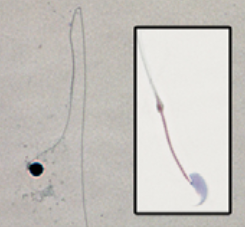
\includegraphics[scale=0.8]{figure/mouse_globo_spz} 

}

\caption[Comparaison entre les spermatozoïdes des
souris sauvages et globozoospermiques]{\textbf{\emph{Comparaison entre les spermatozoïdes
des souris sauvages et globozoospermiques} d'après
{[}\protect\hyperlink{ref-Pierre2012}{194}{]}} : À gauche, le
spermatozoïde d'une souris globozoospermique
\emph{Dpy19l2}\textsuperscript{-/-}. À droite, celui d'une souris
sauvage \emph{Dpy19l2}\textsuperscript{+/+}.\\}\label{fig:pictmouseglobo}
\end{figure}










\newpage

\section{\texorpdfstring{Résultats 1 : Les mécanismes mutationnels
entraînant la délétion au locus de \emph{DPY19L2} chez
l'humain}{Résultats 1 : Les mécanismes mutationnels entraînant la délétion au locus de DPY19L2 chez l'humain}}\label{mecamut}

\subsection{Article n°6:}\label{article-n6}

\textbf{Fine Characterisation of a Recombination Hotspot at the
\emph{DPY19L2} Locus and Resolution of the Paradoxical Excess of
Duplications over Deletions in the General Population}

Coutton C, Abada F, \textbf{Karaouzène T}, Sanlaville D, Satre V,
Lunardi J, Jouk PS, Arnoult C, Thierry-Mieg N, Ray PF

\textsuperscript{*} Co-premiers auteurs

PLOS GeneticS, Mars 2013

\newpage

\subsubsection{Contexte et objectifs}\label{contexte-et-objectifs-5}

Chez les mammifères il existe trois paralogues de \emph{DPY19L2} de
fonctions encore inconnues et un pseudogène présentant une très forte
homologie de séquence (\textgreater{} 95\%)
{[}\protect\hyperlink{ref-Carson2006}{195}{]}. Chez l'homme, ce gène est
flanqué de deux séquences présentant une forte homologie
(\textgreater{}95\%) d'une taille de 28kb. Ces séquences appelées LCRs
(\emph{low copy repeats}) représentent une large portion du génome
humain {[}\protect\hyperlink{ref-Cheung2003}{196},
\protect\hyperlink{ref-Bailey2002}{197}{]} et vont, de par leur
homologie favoriser les duplications de gènes jouant ainsi un rôle
important dans l'évolution des génomes des vertébrés
{[}\protect\hyperlink{ref-Walsh2003}{198},
\protect\hyperlink{ref-Ohno1970}{199}{]}. Dans le cas de \emph{DPY19L2},
ces LCRs vont, au cours de la méiose, entrainer la survenue de
recombinaisons homologues non-allélique (NAHR) donnant lieu soit à une
délétion du gène \emph{DPY19L2} et la formation d'un ADN circulaire
comprenant le gène soit à un allèle possédant deux copies du gène tandis
que l'autre n'en possède aucune
{[}\protect\hyperlink{ref-Harbuz2011a}{200}{]}.

Ce mécanisme de NAHR devrait, en théorie, engendrer la formation de plus
d'allèles délétés que d'allèles dupliqués puisque seuls les remaniments
interchromatidiens les induisent la formation d'un allèle dupliqué
tandis que les délétions surviennent à la fois lors des remanimets
interchromatidiens \textbf{et} intrachromatidiens
{[}\protect\hyperlink{ref-Liu2012}{201}{]} (\textbf{Figure :
}\ref{fig:pictnahr}). Cependant, les données mises à disposition par la
base de données \href{http://dgv.tcag.ca/dgv/app/home}{\emph{Database of
Genomic Variants}} (DGV)
{[}\protect\hyperlink{ref-MacDonald2014}{202}{]} indiquent un excès de
duplication puisque sur un total de 6575 individus analysés, 83
duplications et de 26 délétions hétérozygotes ont été observées pour le
locus de \emph{DPY19L2}.

Ainsi, dans cette étude, notre équipe a cherchée à caractériser
précisément le mécanisme génétique et les facteurs favorisant la
survenue par NAHR de la délétion homozygote récurrente emportant
totalement le gène DPY19L2. De même, nous avons tenté de résoudre le
paradoxe observé entre le modèle théorique de NAHR et la fréquence des
allèles observée dans la population générale afin de confirmer les
données fournies dans les bases de données et ainsi écarter l'hypothèse
d'un biais causé par la présence du pseudogène \emph{DPY19L2P1} très
homologue avec \emph{DPY19L2}
{[}\protect\hyperlink{ref-Carson2006}{195}{]}.

Dans ce contexte j'ai pu participer à diverses manipulations de biologie
moléculaire tel que l'extraction d'ADN spermatique, quantification des
délétions / duplications \emph{de novo}. J'ai également contribué au
diverses analyses statistiques.

\newpage 

\begin{figure}

{\centering \includegraphics[scale=0.5]{figure/nahr_process} 

}

\caption[Représentation schématique du mécanisme de NAHR]{\textbf{\emph{Représentation schématique du mécanisme de
NAHR} adapté d'après {[}\protect\hyperlink{ref-Liu2012}{201}{]}} : Lors
d'un NAHR interchromatidien, un allèle dupliqué et un allèle délété sont
formés. Lors d'un NAHR intrachromatidien, seul un allèle délété est
produit, en même temps qu'un petit ADN circulaire qui sera éliminé par
la suite.}\label{fig:pictnahr}
\end{figure}








\newpage

\includepdf[pages=-]{bib/DPY19L2_2013}

\newpage

\subsubsection{Principaux résultats}\label{principaux-resultats-5}

Contrairement à ce que prédit la théorie de formation des NAHRs, les
résultats extraits des bases de données publiques indiquent un excès
d'allèles dupliqués de \emph{DPY19L2} dans la population générale. Nous
avons donc cherché à déterminer les fréquences des duplications et
délétions \emph{de novo} de ce même locus. Ceci ayant pour but de
déterminer si cet excès est dû à une sélection de l'allèle dupliqué ou
au fait que celui-ci était effectivement produit plus fréquemment que
l'allèle délété. Pour ce faire nous avons quantifié le taux d'apparition
de ces événements génétiques à partir d'ADN spermatique. Les
spermatozoïdes étant le produit direct de la méiose, ils sont donc les
reflets d'haplotypes produits \emph{de novo}. Pour cela, nous avons
analysé par PCR digitale l'ADN spermatique de trois donneurs ainsi que
l'ADN spermatique constitué d'un mix provenant de ces trois donneurs.
Leur ADN a tout d'abord été dilué en série afin qu'environ 25\% des 96
puits de la PCR contiennent un événement (délétion ou duplication).
Ainsi, en acceptant qu'un génome haploïde humain représente 3pg, 50ng
d'ADN spermatique furent déposés dans chaque puit pour la PCR spécifique
à la délétion, et 100ng dans chaque puit spécifique à a duplication.
Chaque puit contient donc une partie de cette charge d'ADN initiale. La
distribution de cette charge d'ADN au sein des 96 puits peut donc
s'apparier à un tirage sans remise, la probabilité qu'un puit soit
positif pour un événement chromosomique (duplication ou délétion) peut
donc être modélisé par une loi hypergéométrique (\textbf{Équation} :
\eqref{eq:hypergeo}). Nous permettant ainsi d'estimer la fréquence
duplication / délétion \(\lambda\) pour chaque donneur
(\textbf{Équation} : \eqref{eq:lambda}).

\begin{equation} 
\frac{\frac{(N - R)!}{W!(N-R-W)!}}{\frac{N!}{W!(N-W)!}} = \frac{(N-R)!(N-W)!}{N!(N-W-R)!} = \prod_{i=0}^{R-1}{\frac{N-W-i}{N-i}}
\label{eq:hypergeo}
\end{equation}

\begin{equation} 
\lambda = \frac{R}{N}
\label{eq:lambda}
\end{equation}

Où :\\
. \(N\) : représente le nombre de copie de chromosome 12 dans la charge
d'ADN initiale (1.6x10\({^6}\) pour la PCR spécifique à la délétion,
3.2x10\({^6}\) pour la PCR spécifique à la duplication)\\
. \(W = \frac{N}{96}\) correspond au nombre de copiede chromosome 12 par
puit\\
. \(R\) représente le nombre total de recombinaison observées

L'intervalle de confiance (IC) à 95\% est ensuite calculé grâce à une
loi binomiale de sorte à modéliser la dilution initiale pour obtenir
l'ADN d'\emph{entrée}. Le puit contenant le \emph{pool} des trois ADN
spermatique est donc celui ayant les résultats les plus robustes, l'IC
étant le plus resserré et permet donc d'établir le taux de délétion
\emph{de novo} à 1.8 x 10\(^{-5}\) (IC 95\% : 1.4x 10\(^{-6}\); 2.2x
10\(^{-6}\)) tandis que le taux de duplication \emph{de novo} est estimé
à 7.7 x 10\(^{-6}\) (IC 95\% : 6.1 x 10\(^{-6}\); 9.7 x 10\(^{-6}\))
montrant un enrichissement environ deux fois supérieur des délétions
\emph{de novo} par rapport aux duplications sur le site de
\emph{DPY19L2}.

Ainsi nous avons observé qu'au locus \emph{DPY19L2} les délétions
\emph{de novo} apparaissent, au cours de la méiose, deux fois plus
fréquemment que les duplications alors que l'allèle dupliqué est trois
fois plus fréquent que l'allèle délété dans la population générale. Cet
effet pourrait en partie être dû aux effets de sélection naturelle. En
effet, Bien qu'à notre connaissance, les femmes portant l'allèle délété
à l'état homozygote ne soient caractérisées par aucun phénotype, les
hommes, eux sont 100\% infertiles tandis que l'allèle dupliqué ne
subirait aucune sélection.

Cette étude a également été pour notre équipe l'occasion d'effectuer une
étude plus approfondie des LCRs flanquants le locus de \emph{DPY19L2}.
Pour cela, nous avons génotypé 20 SNPs spécifiques des LCRs télomériques
et centromériques. À partir de ces données, 5 points de cassures
distincts (BP1-5) ont pu être identifiés sur les 185 allèles recombinés
étudiés (108 délétés et 77 dupliqués). L'ensemble de ces points de
cassures sont localisés dans une région d'environ 1150 pb localisée au
centre des 28kb du LCR. L'analyse bioinformatique de cette région a
permis de mettre en évidence, au centre de la région minimale de
recombinaison un site de reconnaissance consensus de la protéine PRDM9
(CCNCCNTNNCCNC). Cette protéine à doigts de zinc est connue pour son
rôle central dans les mécanismes de recombinaisons homologue au cours de
la méiose chez l'humain et la souris en ciblant de manière spécifique la
localisation des cassures doubles brins, préambule nécessaire à toute
recombinaison {[}\protect\hyperlink{ref-Parvanov2010}{203},
\protect\hyperlink{ref-Baudat2010}{204}{]}. On peut donc penser que la
présence de cette séquence consensus de PRDM9 est la raison pour
laquelle toute les points de cassures observés sont localisés dans cette
région minimale de 1150 nucléotide.

\newpage

\section{Résultat 2 : La transcriptomique}\label{transcriptome}

\subsection{Article n°7:}\label{article-n7}

\textbf{Comparative testicular transcriptome of wild type and
globozoospermic Dpy19l2 knock out mice}

\textbf{Karaouzène T} , El Atifi M, Issartel JP, Grepillat M, Charles
Coutton C, Martinez D, Arnoult C and Ray PF

Basic and Clinical Andrology, 2013

\newpage

\subsubsection{Contexte et objectifs}\label{contexte-et-objectifs-6}

Dans des études précédentes, notre équipe à réussit à démontrer que,
chez la souris, la protéine Dpy19l2 était localisée dans la membrane
interne des noyaux des spermatides pendant la spermatogenèse et qu'elle
était nécessaire pour fixer l'acrosome au noyau
{[}\protect\hyperlink{ref-Pierre2012}{194}{]}. Dans cette même étude,
nous avons pu montrer cette protéine colocalisait avec la protéine Sun5
et que \emph{Dpy19l2} pourrait être un partenaire de \emph{Sun5}
{[}\protect\hyperlink{ref-Pierre2012}{194}{]}. Chez la souris, la
protéine Sun1 est elle aussi nécessaire à la gamétogenèse et est connue
pour permettre l'interaction entre le noyau et les télomères
{[}\protect\hyperlink{ref-Ding2007}{205}{]}. Dans cette étude nous avons
donc cherché à savoir si l'absence de la protéine Dpy19l2 pouvait
entrainer des dérèglements transcriptionnels qui pourraient, entre
autre, expliquer l'absence de la protéine Plcz1 dans les spermatozoïdes
globozoocéphales murins.

De plus, au cours de production des souris \emph{Dpy19l2} KO au sein de
notre laboratoire nous avons pu observer un excès de naissance de souris
mâle lorsque l'on croisait deux souris \emph{Dpy19l}\(^{+/-}\). Ainsi,
en comparant les sexes des souris obtenues lors de 6 premières
naissances (\emph{Birth 1-6}) on observe un total de 28 souris mâles
pour 16 souris femelles. La p-valeur obtenue en effectuant un test de
\(\chi^2\) comparant ces deux effectifs était égale à 0.0486272 laissant
supposer l'existence d'un enrichissement réel, bien que faible, en
souris mâles.

C'est donc afin d'expliquer l'absence de la protéine \emph{Plcz1} dans
les spermatozoïdes des souris \emph{Dpy19l2}\(^{-/-}\) ainsi que
l'enrichissement en souris mâle dans les naissances issues
d'accouplement de souris \emph{Dpy19l2}\(^{+/-}\) que nous avons
effectué une analyse comparative du transcriptome testiculaire de deux
souris \emph{Dpy19l2}\(^{+/+}\) (S1\textsuperscript{+} et
S2\textsuperscript{+}) et deux souris \emph{Dpy19l2}\(^{-/-}\)
(S1\textsuperscript{-} et S2\textsuperscript{-}) ayant pour but de
mettre en évidence d'éventuels dérèglements transcriptionnels chez la
souris KO.

Dans cette étude j'ai pu effectuer l'intégralité des manipulations de
biologie moléculaire telles que la mise en place du protocole de
génotypage des souris, l'extraction de l'ARN testiculaire de souris et
l'analyse sur puce, ainsi que l'intégralité de l'analyse bioinformatique
des résultats.

\newpage

\begin{figure}

{\centering \includegraphics{thesis_files/figure-latex/plotborn-1} 

}

\caption[Quantification des sexes des souris observés lors de
chaque naissance issues d'un croisement de deux souris hétérozygotes
\emph{Dpy19l2}\textsuperscript{+/-}\\]{\textbf{\emph{Quantification des sexes des souris
observés lors de chaque naissance issues d'un croisement de deux souris
hétérozygotes \emph{Dpy19l2}\textsuperscript{+/-}}} : Après 6
naissances, 28 souriceaux mâles sont nés pour seulement 16 femelles,
ainsi le test du \(\chi^2\) comparant ces valeurs donne une p-valeur de
0.0486272.}\label{fig:plotborn}
\end{figure}











\newpage

\includepdf[pages=-]{bib/12610_2013_Article_8.pdf}

\newpage

\subsubsection{Principaux résultats :}\label{principaux-resultats-6}

Pour effectuer ces analyses, nous avons donc extrait l'ARN testiculaire
des 4 souris que nous avons ensuite hybridé sur des puces à ADN
Affymetrix GeneChip® Mouse Exon 1.0 contenant des sondes pour 35.557
gènes murins. Cette étape nous a permis d'obtenir pour chacune des 4
souris les valeurs d'expression testiculaire de l'ensemble de leurs
gènes. Pour chacun de ces gènes, nous avons donc cherché à savoir s'ils
étaient différentiellement exprimés chez les souris
S1\textsuperscript{-} et S2\textsuperscript{-} lorsqu'on comparait leur
expression avec celle des souris S1\textsuperscript{+} et
S2\textsuperscript{+}. Pour cela, nous avons calculé quatre ratios (R1,
R2, R3 et R4) (\textbf{Équation} : \eqref{eq:micerate}). Les gènes pour
lesquels au moins 3 de leurs ratios étaient \(\ge\) 1,7 furent
considérés comme sur-exprimés tandis que ceux pour lesquels 3 de leurs
ratio étaient \(\le\) 0,58 (\(\frac{1}{1,7}\)) furent considérés comme
sous-exprimés.

\begin{equation} 
\begin{split}
\forall gene \in & \ \{genes\ in\ array\}: \\
\\
& R1_{gene} = \frac{exp_{gene}(S1^-)}{exp_{gene}(S1^+)} \ \ \ \ R2_{gene} = \frac{exp_{gene}(S2^-)}{exp_{gene}(S1^+)} \\
& R3_{gene} = \frac{exp_{gene}(S1^-)}{exp_{gene}(S2^+)} \ \ \ \ R4_{gene} = \frac{exp_{gene}(S2^-)}{exp_{gene}(S2^+)} 
\label{eq:micerate}
\end{split}
\end{equation}

De cette manière cette étude a pu mettre en évidence la sous-expression
de 6 gènes (incluant \emph{Dpy19l2}) et la sur-expression de 70 gènes
chez les souris \emph{Dpy19l2}\(^{-/-}\). \emph{Plcz1} ne figurait pas
parmi ces gènes indiquant que l'absence de cette protéine chez les
spermatozoïdes globozoocéphales n'étaient pas due à un dysfonctionnement
transcriptionnel.

Afin de prédire les fonctions moléculaires dans lesquels étaient
impliqués ces gènes, nous nous sommes servis du logiciel PANTHER
{[}\protect\hyperlink{ref-Mi2017}{162}{]}. Ainsi, nous avons pu
constater que 23 gènes codant pour des protéines de liaison étaient
dérégulés (\textbf{Figure : }\ref{fig:plotmolfunction} - \textbf{A}),
dont sont des protéines de liaison aux acides nucléiques (\textbf{Figure
: }\ref{fig:plotmolfunction} - \textbf{B}) suggérant que \emph{Dpy19l2}
pourrait effectivement interagir avec l'ADN. D'autres fonctions
moléculaires telles que l'activité catalytique, la régulation de la
transcription et des protéines ayant des fonctions structurelles étaient
également dérégulées chez les souris KO. Ces fonctions sont
particulièrement intéressantes lorsque l'on sait que les spermatozoïdes
globozoocéphales sont caractérisés par plusieurs défauts structurels.

Cette étude a pour nous été l'occasion de mieux caractériser la protéine
\emph{Dpy19l2} chez la souris. Nous avons ainsi pu montrer que les
souris \emph{Dpy19l2}\(^{-/-}\) présentaient des dérèglements
transcriptionnels affectant plusieurs fonctions moléculaires pouvant
potentiellement expliquer, du moins en partie, les nombreux défauts
morphologiques caractérisant les spermatozoïdes globozoocéphales. De
même, nous avons pu observer le dérèglement de nombreux gènes impliqués
dans la liaison d'acide nucléique et de protéine pouvant ainsi expliquer
les défauts d'ancrage de l'acrosome au noyau chez les spermatozoïdes
globozoocéphales.

Ces résultats ne nous ont cependant pas permis d'expliquer l'absence de
la protéine Plcz1 dans le spermatozoïde globozoocéphale murin
l'expression du gène \emph{Plcz1} n'ayant montré aucune dérégulation
chez la souris \emph{Dpy19l2}\textsuperscript{-/-}. De même, aucun des
gènes retrouvés comme dérégulés ne nous a permis d'expliquer le biais de
sexe que nous avions observés. Cela n'a pas été une surprise pour nous
puisque après avoir entamé notre étude, une dernière portée issues d'un
croisement de souris \emph{Dpy19l2}\textsuperscript{+/-} a vue le jours.
Celle-ci état composée de 4 souriceaux mâles et de 4 souriceaux
femelles. Ainsi, avec un total de 32 souris mâles pour 20 souris
femelles, la p-valeur de notre test du \(\chi^2\) à 0.0635765 laissant
cette fois-ci supposer la non-existence d'un biais de sexe dans les
naissances issues d'un croisement de souris
\emph{Dpy19l2}\textsuperscript{-/-}.

\newpage 

\begin{figure}

{\centering \includegraphics{thesis_files/figure-latex/plotmolfunction-1} 

}

\caption[Principales fonctions moléculaires affectées
chez les souris \emph{Dpy19l2} KO\\]{\textbf{\emph{Principales fonctions moléculaires
affectées chez les souris \emph{Dpy19l2} KO}} : \textbf{A} : Liste des
fonctions moléculaires affectées : Bndn = Binding, Ctly = Catalytic,
Trnsc = Transcription, Strm = Structural molecule, Rcpt = Receptor.
\textbf{B} : Détails des fonctions moléculaires affectées par les gènes
dérégulés.}\label{fig:plotmolfunction}
\end{figure}










\chapter*{Conclusion et discussion}\label{conclusion-et-discussion}
\addcontentsline{toc}{chapter}{Conclusion et discussion}

L'infertilité est une problématique qui concerne entre 10 et 15\% des
couples {[}\protect\hyperlink{ref-Boivin2007a}{34}{]} faisant de cette
pathologie un enjeu de santé publique. Bien que les causes de ce
phénotype puissent être multifactorielles et acquises au cours de la vie
de l'l'individu, notamment suite à des infections du système urogénitale
ou encore à des perturbations du système endocrinien, la composante
génétique est extrêmement importante. À ce jour, malgré les efforts de
nombreuses équipes, incluant la notre, seulement une poignée de gènes a
pu être reliée à ce phénotype. De plus, pour nombre d'entre eux, les
bases moléculaires reliant une mutation au phénotype d'infertilité
restent inconnues. Ces quinze dernières années, les techniques
d'investigation employées dans les analyses phénotypes-génotype, ont été
boulversées par l'emmergence du séquençage haut-débit. En effet, ces
technologies permettent aujourd'hui de séquencer l'ensemble du génome /
exome d'un individu pour un coût et dans un temps raisonnable.
Malheuresement, la masse de données générées par ces méthodes, bien qu'à
l'origine du succès de celles-ci, deviennent aujourd'hui un frein dans
l'analyse et la compréhension des processus biologiques étudiés.

Dans ce contexte, j'ai pu, au cours de ma thèse, mettre au point un
pipeline permettant l'analyse des données issues de séquençage NGS. Ce
pipeline a ainsi permis, entre 2012 et 2017, l'analyse des données de
nombreux patients présentant tous un phénotype d'infertilité. Celle-ci
ayant pour vocation première de mettre en évidence les variants
responsables des phénotypes de ces patients. Contrairement à la plupart
des pipelines d'analyse de données WES existant, celui-ci prend en
charge l'ensemble des étapes de l'analyse allant de l'alignement des
\emph{short-reads} sur le génome de référence jusqu'à la priorisation
des variants en passant par l'appel des variants et leur annotation. Les
résultats de chacune de ces étapes pouvant être contrôlées et
personnalisées grâce à des paramètres ajustables. L'alignement des
\emph{reads} est effectué par le logiciel MAGIC tandis que les variants
et leur génotype sont appelés par un algorithme développé dans notre
laboratoire spécifiquement conçu pour analyser les informations fournies
par MAGIC et dont les paramètres sont ajustables en fonctions de la
distribution des pourcentages de \emph{reads} variants observés dans les
données analysées. Pour l'annotation nous avons utilisé plusieurs
ressources extérieures tel que le logiciel Variant Effect Predictor qui
va nous informer de l'effet d'un variant sur l'ensemble des transcrits
qu'il chevauche. De même, les bases de données ExAC ESP6500 ou encore
1KG nous donne une indication de la fréquence des variants dans la
population générale. Une fois ces étapes effectuées, nous avons mis en
place plusieurs filtres successifs afin d'éliminer de nos listes les
variants ayant le moins de chances d'être responsables du phénotype des
différents patients. Ceux-ci s'appuient à la fois sur les critères
qualité des résultats de séquençage, le génotype des variants, leur
fréquence ou encore leur impact sur la protéine.

L'efficacité de ce pipeline a pu être démontré grâce à son utilisation
sur des cas familiaux mais aussi sur des cohortes d'individus non
apparentés. Ainsi, nous avons pu dans un premier temps confirmer
l'importance de l'implication du gène \emph{DNAH1} dans le syndrome MMAF
en le retrouvant muté chez 9 de nos patients (4 au sein d'études
familiales et 5 parmi notre cohorte d'individus non apparentés).
Ensuite, dans un second temps, ce pipeline nous a permis de mettre en
évidence un total de 5 nouveaux gènes dans des phénotypes d'infertilité
masculine et féminine. Ainsi les gènes \emph{CFPA43}, \emph{CFAP44},
retrouvés respectivement mutés à chez 10 (9 homozygotes et 1
hétérozygote composite) et 6 (tous homozygotes) de nos patients ont pu
être liés à leur syndrome MMAF. Aussi, une même mutation impactant le
gène \emph{PATL2} a pu être reliée au phénotype de déficience méiotique
ovocytaire de cinq femmes. Pour finir, des mutations sur les gènes
\emph{SPINK2} et \emph{PLCZ1} ont, elles aussi, pu être liées aux
phénotypes d'azoospermie et d'echec de fécondation dont étaient atteint
deux fratries.

Dans autre partie de mon travail de thèse j'ai pu prendre part à la
caractérisation génétiques et moléculaires du gène \emph{DPY19L2}
impliqué dans le phénotype de globozoospermie. Ce phénotype, entrainant
la production de 100\% de spermatozoïdes à têtes rondes et dépourvus
d'acrosomes est principalement causé, chez l'humain, par une délétion
homozygote récurrente entrainant la perte de la totalité de la séquence
du gène \emph{DPY19L2}. Ainsi, dans deux études différentes, nous avons
pu, dans un premier temps, mieux caractériser les mécanismes
moléculaires responsables de cette délétion. Ainsi, nous avons pu mettre
en évidence cinq points de cassures au niveau des LCRs flanquant la
séquence de \emph{DPY19L2} chez l'humain. Ceux-ci étant tous concentrés
dans une région d'environ 1150 pb contenant en son centre un site de
reconnaissance consensus de la protéine PRDM9 connue pour son
implication dans la recombinaison chromosomique chez l'humain et la
souris {[}\protect\hyperlink{ref-Parvanov2010}{203},
\protect\hyperlink{ref-Baudat2010}{204}{]}. Cette même étude a également
permis de démontrer que les effets de la sélection naturelle étaient
responsables du paradoxe observé dans la population générale : une
fréquence plus élevée d'allèles dupliqués comparativement aux allèle
délétés au locus DPY19L2 tandis que \emph{de novo}, l'allèle délété est
produit, en théorie et en pratique, plus fréquemment que l'allèle
dupliqué. L'étude de ce phénotype nous a par la suite poussée à étudier
le modèle murin KO \emph{Dpy19l2}\textsuperscript{-/-} présentant le
même phénotype que l'humain. Afin d'expliquer l'absence de la protéine
PLCZ1 chez l'humain globozoosperme, nous avons effectué une analyse
comparative des transcriptomes testiculaires de souris sauvages
\emph{Dpy19l2}\textsuperscript{+/+} et KO
\emph{Dpy19l2}\textsuperscript{-/-}. Bien qu'aucun dérèglement
transcriptionnel n'ait pu être observé pour le gène \emph{Plcz1} cette
étude nous a permis de mettre en évidence un total de 75 gènes
présentant des dérégulations transcriptionnelles pouvant expliquer en
partie les anomalies physiologiques et morphologiques des spermatozoïdes
des souris\emph{Dpy19l2}\textsuperscript{-/-}.

Au cours des différents travaux réalisés au cours de ma thèse, nous
avons pu constater la puissance des technologies de séquençage
haut-débit. En effet, en seulement 5 ans, celles-ci ont permis
l'identification de 5 nouveaux gènes impliqués dans des phénotypes
d'infertilité au sein de notre laboratoire. Ces résultats sont cependant
à relativiser puisque qu'aucun candidat n'a pu être identifié pour 68\%
des patients analysés. Plusieurs raisons peuvent expliquer cela. Tout
d'abord, au cours des analyses décrites dans ces manuscrits nous nous
concentrons uniquement sur les SNPs et les indels. Cependant de nombreux
logiciels tel que ExomeDepth
{[}\protect\hyperlink{ref-Plagnol2012}{206}{]}, CoNIFER
{[}\protect\hyperlink{ref-Krumm2012}{207}{]} ou encore ExomeCNV
{[}\protect\hyperlink{ref-Sathirapongsasuti2011}{208}{]} permettent de
détecter des CNVs à partir de données WES et / ou WGS. Les stratégies de
prédictions de ces logiciels pouvant être extrêmement différents
(\textbf{Figure : }\ref{fig:pictcnvdetection}), le profil des CNVs
détectés ou non le sera aussi {[}\protect\hyperlink{ref-Zhao2013}{209},
\protect\hyperlink{ref-Guo2013}{210}{]}. Ainsi, dans des analyses non
décrites dans ce manuscrit, j'ai pu chercher à identifier des CNVs à
partir de nos données d'exome à l'aide du logiciel ExomeDepth
{[}\protect\hyperlink{ref-Plagnol2012}{206}{]}. Cette approche a été
extrêmement concluante puisqu'elle a permis d'identifier une délétion
homozygote sur le gène \emph{WDR66} chez 7 de nos patients pour lesquels
aucun candidat n'avait été alors identifié. Ces délétions ont ensuite pu
être confirmées par PCR et la caractérisation de ce gène est
actuellement en cours au sein de notre équipe. Au vu de cette réussite,
il est désormais prévu d'intégrer ce genre d'analyse de manière
automatique et systématique au sein de notre pipeline.

\newpage

\begin{figure}

{\centering \includegraphics[scale=0.55]{figure/cvn_detection_strategies} 

}

\caption[Présentation de cinq approches permettant la détection de CNVs à partir de données NGS]{\textbf{\emph{Présentation de cinq approches
permettant la détection de CNVs à partir de données NGS} d'après
{[}\protect\hyperlink{ref-Zhao2013}{209}{]}} : \textbf{A} : Cette
stratégie, permet de prédire des CNVs à partir des alignements
discordants des deux \emph{ends} d'un même \emph{read}, c'est à dire en
répertoriant les \emph{reads} pour lesquels la distance séparant les
deux \emph{ends} après l'alignement est significativement supérieure à
la taille moyenne de l'insert. \textbf{B} : La méthode \emph{split-read}
se base sur les \emph{reads} s'alignant de manière partielle sur
plusieurs régions génomiques. \textbf{C} : L'approche \emph{read depth}
compare la couverture observée sur plusieurs régions génomiques pour
prédire des CNVs. \textbf{D} : Cette méthode effectue un assemblage
\emph{de novo} (sans utilisé de génome de référence) ; les résultats de
l'assemblage appelés \emph{contigs} sont comparés au génome de référence
a posteriori pour détecter les CNVs. \textbf{E} : Cette méthode combine
les approches \textbf{A} et \textbf{C}.}\label{fig:pictcnvdetection}
\end{figure}


















\newpage

Pour les patients n'ayant eu aucun candidat identifié, il est possible
que le choix de la stratégie du séquençage exomique plutôt que du génome
entier ait masqué la cause génétique du phénotype de certains de nos
patients. En effet, dans ces analyses, nous nous sommes concentrés sur
l'analyse des variants situés dans les parties codantes
\textbf{uniquement}. Ainsi les variants situés par exemple dans les
microARN n'ont pu être observés. Or, les microARN jouent un rôle
important dans la régulation génique principalement en influant sur la
stabilité d'ARNm cibles et sont présent en grande quantité au sein des
cellules germinales et leur importance dans la spermatogenèse a déjà été
démontrée chez la souris
{[}\protect\hyperlink{ref-Comazzetto2014}{211}{]} ainsi que plus
récemment chez d'autres mammifères dont l'humain
{[}\protect\hyperlink{ref-Chen2017}{212}{]} laissant penser que des
défauts altérants ces microARN pourraient entrainer des
dysfonctionnements de la spermatogenèse. Aussi, il faut noter que les
analyses WES \textbf{et} WGS ne permettent pas d'observer les défauts
épigénétiques, or, ceux-ci représentent une part croissante des causes
impliquées dans les cas d'infertilité masculine
{[}\protect\hyperlink{ref-Carrell2011}{213}--\protect\hyperlink{ref-Dada2012}{215}{]}.
Aussi, au vu du grand nombre de gènes impliqués dans la spermatogénèse
il est très possible que les causes génétiques responsables d'un même
phénotype puissent être très hétérogènes. Par exemple, dans le cas de
l'analyse de la cohorte de patients MMAF, 3630 variants subsistaient
après avoir appliqué l'ensemble des filtres. Ces variants impactaient
2780 gènes différents parmi lesquels 1684 étaient retrouvés mutés chez
uniquement un seul des 78 patients de la cohorte. Au vu de ce nombre
important de gènes, il est très compliqué d'effectuer des analyses
poussées sur l'ensemble d'entre eux. Dès lors, il est possible que la
cause génétique responsable du phénotype d'un patient soit ``noyée''
parmi les nombreux variants restant mettant ainsi en évidence la
nécessité de créer de nouveaux filtres afin de pouvoir réduire encore
cette liste.

C'est dans ce but que notre équipe travaille actuellement au
développement du score MutaScript. Ce score a pour but de classer
l'ensemble des transcrit codant en fonction de leur charge mutationnelle
avec l'idée sous-jacente que les transcrits les plus mutés dans la
population générale ne sont probablement pas impliqués dans des
pathologies sévères à transmission Mendélienne, et \emph{a contrario}
ceux retrouvés comme n'étant pas / peu mutés le sont probablement. Pour
ce faire, le score MutaScript repose sur trois informations principales.
La première étant le jeu de transcrits fournit par Ensembl
{[}\protect\hyperlink{ref-Aken2017}{175}{]}. Afin de connaitre la charge
mutationnelle de ces transcrits, nous nous sommes basées sur les
variants mis à disposition par ExAC
{[}\protect\hyperlink{ref-Lek2016}{151}{]} qui réunit les données
d'exome de 60.706 individus non apparentés que nous avons ensuite annoté
grâce au logiciel \emph{variant effect predictor} (VEP)
{[}\protect\hyperlink{ref-McLaren2016}{152}{]} afin de prédire l'impact
de chaque variant sur l'ensemble des transcrits qu'ils chevauchent de
sorte à ce que les variants ayant un impact prédit comme étant délétère
aient une plus grosse contribution au score MutaScript que ceux ayant un
impact faible. Ces dernières années, des scores tel que le
\emph{residual variance intolerance score} (RVIS)
{[}\protect\hyperlink{ref-Petrovski2013}{164}{]} ou encore \emph{the the
Probability of loss-of-function Incoherency} (pLI)
{[}\protect\hyperlink{ref-Lek2016}{151}{]} ont vu le jour. MutaScript se
présente comme une alternative à ces derniers scores et, bien que sa
fonction soit similaire, il diffère de ceux-ci sur de nombreux points.
Tout d'abord, MutaScript donne un score à l'ensemble des transcrits
codant pour une protéine là où pLI donne un score seulement au transcrit
consensus de chaque gène et RVIS qui agrège les séquences codantes de
l'ensemble des transcrits d'un même gène créant ainsi un transcrit
``chimérique''. Ce procédé facilite l'interprétation du score mais
engendre une perte d'information puisque l'on se retrouve avec un seul
score par gène et non par transcrits. De plus, dans la conception de
leur score, RVIS et pLI ne considèrent que les variants dit
\emph{loss-of-function} (LoF), c'est à dire les variants impactant
l'épissage, engendrant un codon stop ou un décalage du cadre de lecture.
Cependant, ces variants ne représentent qu'une faible proportion des
variants fournis par la base de données ExAC. C'est pourquoi, MutaScript
prend en compte l'ensemble des variants, quelque que soit leur impact
sur les différents transcrits qu'ils chevauchent, et leur attribue un
poids en fonction de cet impact de sorte à ce que les variants
considérés comme étant les plus délétères contribuent plus au score d'un
transcrits que les autres. Aussi, l'étude des scores RVIS et pLI nous a
permis de mettre en évidence une corrélation forte entre le score qu'ils
attribuent à un gène et la taille de la séquence codante (CDS) de ce
même gène. Cette corrélation étant due à un biais causé par leur manière
de calculer leur score et non à une réalité biologique, MutaScript est
construit de sorte à éviter cette corrélation qui peut mener à des
erreurs d'interprétations. Le développement de ce score est en cours de
finalisation.

Après avoir fait ses preuves dans la recherche, le séquençage NGS joue
un rôle de plus en plus important dans le domaine du diagnostic clinique
et on peut logiquement penser que ces technologies remplaceront bientôt
la plupart des techniques diagnostiques actuelles. Il est néanmoins
légitime de se demander dès aujourd'hui quelle sera son efficacité. En
effet, en se basant sur les données de nos 78 patients non apparentés
souffrant du syndrome MMAF on peut s'attendre, à obtenir entre 747 et
2499 variants par patients avec un coefficient de variation de 29\%
(avec \(C_v = \frac{\sigma}{\mu}\) où \(\sigma\) est l'écart-type et
\(\mu\) la moyenne). Ces chiffres sont obtenus en filtrant de notre
ensemble de variants ceux ayant une fréquence \(\ge\) 0.01 dans les
bases de données publiques ainsi qu'en retirant les variants
introniques, synonymes et ceux impactant les séquences UTRs. On constate
alors que parmi l'ensemble de ces variants \texttt{rn\_var\_unique}
d'entre eux (26\%) sont ``individuels'', c'est à dire porté uniquement
par un seul des patients (\textbf{Figure : }\ref{fig:plotvarperimpact} -
\textbf{A}). De même on peut observer que chacun de nos patients est
porteur d'environ 153 variants tronquants parmi lesquels 78 le sont à
l'état homozygote (\textbf{Figure : }\ref{fig:plotvarperimpact} -
\textbf{B}). La priorisation de certains gènes par des outils tel que
MutaScript permettra alors d'orienter les analyses vers les gènes les
plus prometteurs. De même la recherche de variants parmi des panels de
gènes permettra également de cibler les recherches sur les gènes déjà
connus comme étant lié au phénotype en question. Ainsi, au vu de nos
résultats dans le cadre de patients atteins du syndrome MMAF, la
recherche de variants dans les gènes \emph{DNAH1}, \emph{CFAP43},
\emph{CFAP44} et \emph{WDR66} permettrait d'obtenir un diagnostic
positif dans environ 36\% des cas. On peut dès lors s'attendre que les
recherches futures vont permettre d'agrandir cette liste de gènes cibles
améliorant ainsi l'efficacité du diagnostic.

\newpage

\begin{figure}

{\centering \includegraphics{thesis_files/figure-latex/plotvarperimpact-1} 

}

\caption[Analyse des variants restant sur chacun des 78 patients après filtrage]{\textbf{\emph{Analyse des variants restant sur
chacun des 78 patients après filtrage}} : \textbf{A} : Répartition du
nombre de patients portant un même variant. Les variants portés par 10
patients ou plus sont regroupés sous l'étiquette 10+. On voit ici
clairement qu'une grande majorité des variants sont spécifiques à un
seul patient. \textbf{B} : Sur cette figure chaque point représente un
patient. Les variants homozygote sont représentés en rouge, les variants
hétérozygotes en bleu. L'impact \emph{LOW} correspond aux variants ayant
un impact peu délétère sur le gène tel que les variants intonique situés
dans les zones d'épissage lointaines. Les variants \emph{MODERATE} tel
que les faux-sens ont un impact modéré sur le gène. Les \emph{HIGH}
représentent les variant tronquants (décalage du cadre de lecture, codon
stop\ldots{}).}\label{fig:plotvarperimpact}
\end{figure}















\newpage

\begin{center}\rule{0.5\linewidth}{\linethickness}\end{center}

Pendant de nombreuses années, la Science et la Technique étaient
considérées comme des disciplines distinctes. Elles étaient pratiquées,
dans la grande majorité des cas, de manière indépendante l'une de
l'autre et surtout par des personnes différentes n'entretenant que peu
d'interactions. Bien que la distinction entre Science et Technique soit
réelle, la première pouvant être définie comme la quête de la
connaissance et de la compréhension du monde tandis que la seconde met
en œuvre un ensemble de moyen afin de modifier celui-ci d'une manière
déterminée à l'avance, l'interdépendance liant ces deux notions n'a
jamais été aussi forte qu'à notre époque tant et si bien qu'elles sont
souvent confondues. En effet, il est courant d'entendre parler de
progrès scientifique pour présenter une innovation technologique et
\emph{vice versa}. Ainsi, si la Science n'est pas la Technique, elle est
dans de nombreux cas dépendante de celle-ci. En effet, comme nous avons
pu le voir, l'étude et la connaissance du génome ont dû attendre les
progrès techniques permettant notamment le séquençage de l'ADN. La
Technique, elle, n'a pas nécessairement besoin de savoirs scientifiques
pour être conçue : des savoirs empiriquement acquis suffisent à
l'application d'une technique. Par exemple, bien qu'ils n'aient eu
aucune conscience des mécanismes scientifiques sous-jacents, les
premiers hommes ont su maitriser plusieurs techniques de production et
d'entretien du feu. De la même manière les agriculteurs n'ont pas eu
besoin d'attendre et de comprendre les travaux sur la génétique et
l'hérédité pour observer que la mise en reproduction des bêtes les plus
productives permettait de maximiser les chances que la descendance soit
elle aussi très productive. Cependant la Technique utilise de plus en
plus des connaissances scientifiques et a ainsi finit par beaucoup
dépendre d'elle en utilisant et appliquant des savoirs scientifiques.
Ainsi est née la Technologie. Les travaux décrits dans ce manuscrit
illustrent parfaitement cette relation d'interdépendance entre la
Science et le Technique / Technologie. En effet, la connaissance du
génome a été permise par l'émergence des différentes technologies de
séquençage qui s'appuient elles aussi sur de nombreuses connaissances
scientifiques. On peut dès lors s'attendre à ce que Science et
Techniques / Technologie continuent d'évoluer de manière concomitante en
s'entre alimentant. Dès lors, on peut prédire que les prochains progrès
technologiques seront à l'origine de découvertes scientifiques qui
serviront elles même à la fois de socle mais aussi de guide aux
évolutions technologiques futures.

\appendix

\hypertarget{dnah12014}{\chapter{Article annexe}\label{dnah12014}}

\textbf{Mutations in DNAH1, which Encodes an Inner Arm Heavy Chain
Dynein, Lead to Male Infertility from Multiple Morphological
Abnormalities of the Sperm Flagella}

Ben Khelifa M\textsuperscript{*}, Coutton C\textsuperscript{*}, Zouari
Raoudha, \textbf{Karaouzène T}, Rendu J, Bidart M, Yassine S, Pierre V,
Delaroche J, Hennebicq S, Grunwald D, Escalier D, Pernet-Gallay K, Jouk
PS, Thierry-Mieg N, Touré A, Arnoult C, Ray PF

American Journal of Human Genetics, Janvier 2014

\textsuperscript{*} Co-premiers auteurs

\newpage

\includepdf[pages=-]{bib/DNAH1_2014.pdf}

\newpage

\newpage

\chapter{Tables des variants restant après application des filtres pour
les cas
familliaux}\label{tables-des-variants-restant-apres-application-des-filtres-pour-les-cas-familliaux}

\begin{longtable}[t]{lll}
\caption{\label{tab:tabmmaf1}Liste des variants ayant passé l'ensemble des filtres pour les deux fères P1 et P2 de la famille MMAF1}\\
\toprule
\multicolumn{1}{c}{ } & \multicolumn{2}{c}{Variant impact} \\
\cmidrule(l{2pt}r{2pt}){2-3}
SYMBOL & HGVSc, HGVSp & Consequence\\
\midrule
PLA2G4B & c.1710-6delA ; . & splice region\\
\bottomrule
\end{longtable}

\begin{longtable}[t]{lll}
\caption{\label{tab:tabmmaf2}Liste des variants ayant passé l'ensemble des filtres pour les deux fères P3 et P4 de la famille MMAF2}\\
\toprule
\multicolumn{1}{c}{ } & \multicolumn{2}{c}{Variant impact} \\
\cmidrule(l{2pt}r{2pt}){2-3}
SYMBOL & HGVSc, HGVSp & Consequence\\
\midrule
SEMA5B & c.658C>A ; p.Glu220Lys & missense\\
CCDC37 & c.1234\_1236delTGG ; p.Glu412del & inframe deletion\\
DAPK1 & c.2431T>A ; p.Val811Met & missense\\
MTSS1L & . ; p.Arg609Trp & missense\\
HYDIN & c.14857>T ; p.Arg4953Trp & missense\\
\addlinespace
TMEM231 & . ; p.Ala71Val & missense\\
ZNF469 & . ; p.Arg1864Lys & missense\\
TGIF2 & c.496C>A ; p.Leu166Met & missense\\
MMP9 & c.820G>A ; p.Glu274Lys & missense\\
\bottomrule
\end{longtable}

\begin{longtable}[t]{lll}
\caption{\label{tab:tabmmaf3}Liste des variants ayant passé l'ensemble des filtres pour les deux fères P5 et P6 de la famille MMAF3}\\
\toprule
\multicolumn{1}{c}{ } & \multicolumn{2}{c}{Variant impact} \\
\cmidrule(l{2pt}r{2pt}){2-3}
SYMBOL & HGVSc, HGVSp & Consequence\\
\midrule
MYH11 & c.4625G>A ; p.Arg1542Gln & missense\\
DNAH1 & . ; . & splice acceptor\\
\bottomrule
\end{longtable}

\begin{longtable}[t]{lll}
\caption{\label{tab:tabmmaf4}Liste des variants ayant passé l'ensemble des filtres pour les deux fères P8 et P9 de la famille MMAF4}\\
\toprule
\multicolumn{1}{c}{ } & \multicolumn{2}{c}{Variant impact} \\
\cmidrule(l{2pt}r{2pt}){2-3}
SYMBOL & HGVSc, HGVSp & Consequence\\
\midrule
WEE2 & . ; p.Pro92Leu & missense\\
GBP2 & c.412T>A ; p.Ala138Thr & missense\\
ZFYVE28 & c.1729C>A ; p.Val577Met & missense\\
FCGR3A & c.133T>C ; p.Ala45Pro & missense\\
\bottomrule
\end{longtable}

\newpage

\begin{longtable}[t]{lll}
\caption{\label{tab:tabmmaf5}Liste des variants ayant passé l'ensemble des filtres pour le patient P10 de la famille MMAF5}\\
\toprule
\multicolumn{1}{c}{ } & \multicolumn{2}{c}{Variant impact} \\
\cmidrule(l{2pt}r{2pt}){2-3}
SYMBOL & HGVSc, HGVSp & Consequence\\
\midrule
ALOX15 & c.268T>C ; p.Asp90His & missense\\
NFATC4 & . ; p.Glu577Gly & missense\\
MYH7 & c.77G>T ; p.Ala26Val & missense\\
LDHAL6A & c.334A>T ; p.Arg112Ter & stop gained\\
GBF1 & c.1588G>T ; p.Arg530Cys & missense\\
\addlinespace
TRBV6-6 & c.5A>T ; p.Ser2Ile & missense\\
MROH2A & . ; p.Ile180Thr & missense\\
FSIP2 & . ; p.Ala86Val & missense\\
ZSWIM2 & c.676G>A ; p.Leu226Met & missense\\
CPZ & c.1236A>T ; p.Lys412Asn & missense\\
\addlinespace
CCDC73 & c.851A>C ; p.Phe284Ser & missense\\
NXPE2 & c.1595>T ; p.Thr532Met & missense\\
NKX2-1 & c.843G>T ; p.Gln281His & missense\\
CASP8 & c.74A>G ; p.Pro25Arg & missense\\
OR6S1 & . ; p.Leu116Met & missense\\
\addlinespace
PDZD7 & . ; p.Ser324Asn & missense\\
COL27A1 & c.5063G>A ; p.Arg1688Gln & missense\\
SPEF2 & c.3240delG ; p.Phe1080LeufsTer2 & frameshift\\
ACAP1 & c.1597A>T ; p.Arg533Trp & missense\\
C6 & c.2312C>A ; p.Gly771Asp & missense\\
\addlinespace
SLIT1 & . ; . & splice region\\
ARHGAP19-SLIT1 & c.*1721-7A>T ; . & splice region\\
DNAH2 & . ; p.Arg2538Gln & missense\\
\bottomrule
\end{longtable}

\chapter{\texorpdfstring{Table des variants retrouvés sur le gène
\emph{PATL2}}{Table des variants retrouvés sur le gène PATL2}}\label{table-des-variants-retrouves-sur-le-gene-patl2}

\begin{longtable}[t]{llll}
\caption{\label{tab:tabpatl2}Table des variants retrouvés sur le gène \textit{PATL2}}\\
\toprule
\multicolumn{2}{c}{ } & \multicolumn{2}{c}{Variant impact} \\
\cmidrule(l{2pt}r{2pt}){3-4}
Patient & Geno & HGVSc, HGVSp & Consequence\\
\midrule
Ghs103 & Homo & c.478G>T ; p.Arg160Ter & stop gained\\
Ghs104 & Homo & c.478G>T ; p.Arg160Ter & stop gained\\
Ghs114 & Homo & c.478G>T ; p.Arg160Ter & stop gained\\
Ghs5 & Homo & c.478G>T ; p.Arg160Ter & stop gained\\
Ghs98 & Homo & c.478G>T ; p.Arg160Ter & stop gained\\
\bottomrule
\end{longtable}

\newpage

\chapter{Variants retrouvés au sein de notre cohorte de patients
MMAF}\label{variants-retrouves-au-sein-de-notre-cohorte-de-patients-mmaf}

\newpage

\begin{landscape}
\begin{longtable}[t]{llllll}
\caption{\label{tab:tabcfap43}Variants homozygotes retrouvés sur le gène \textit{CFAP43}}\\
\toprule
\multicolumn{2}{c}{ } & \multicolumn{2}{c}{Variant impact} & \multicolumn{1}{c}{Variant frequency} \\
\cmidrule(l{2pt}r{2pt}){3-4} \cmidrule(l{2pt}r{2pt}){5-5}
Patient & Geno & HGVSc, HGVSp & Consequence & SIFT ; PolyPhen & ExAC ; ESP ; 1KG\\
\midrule
Ghs162 & Homo & c.1240\_1241delGC ; p.Val414LeufsTer46 & frameshift & . ; . & . ; . ; .\\
Ghs164 & Homo & c.1240\_1241delGC ; p.Val414LeufsTer46 & frameshift & . ; . & . ; . ; .\\
Ghs25 & Homo & c.2141+5T>A ; p.Lys714Val*11 & splice region & . ; . & . ; . ; .\\
Ghs17 & Homo & c.2658G>A ; p.Trp886Ter & stop gained & . ; . & 9.88e-05 ; 2e-04 ; .\\
Ghs41 & Homo & c.2680C>T ; p.Arg894Ter & stop gained & . ; . & 8.24e-06 ; . ; .\\
\addlinespace
Ghs126 & Homo & c.3352C>T ; p.Arg1118Ter & stop gained & . ; . & 3.29e-05 ; . ; .\\
Ghs105 & Homo & c.3541-2A>C ; p.Ser1181Lysfs*4 & splice acceptor & . ; . & . ; . ; .\\
Ghs160 & Homo & c.3541-2A>C ; p.Ser1181Lysfs*4 & splice acceptor & . ; . & . ; . ; .\\
Ghs102 & Homo & c.3882delA ; p.Glu1294AspfsTer47 & frameshift & . ; . & . ; . ; .\\
Ghs132 & Hete & c.1040G>C ; p.Val347Ala & missense & tolerated ; possibly damaging & 7.41e-05 ; 2e-04 ; .\\
Ghs132 & Hete & c.1300\_1301insT ; p.Leu435SerfsTer26 & frameshift & . ; . & . ; . ; .\\
\bottomrule
\end{longtable}
\end{landscape}

\newpage

\begin{longtable}[t]{llll}
\caption{\label{tab:tabcfap44}Variants homozygotes retrouvés sur le gène \textit{CFAP44}}\\
\toprule
\multicolumn{1}{c}{ } & \multicolumn{2}{c}{Variant impact} & \multicolumn{1}{c}{Variant frequency} \\
\cmidrule(l{2pt}r{2pt}){2-3} \cmidrule(l{2pt}r{2pt}){4-4}
Patient & HGVSc, HGVSp & Consequence & ExAC ; ESP ; 1KG\\
\midrule
Ghs155 & c.1387G>T ; p.Glu463Ter & stop gained & . ; . ; .\\
Ghs177 & c.1387G>T ; p.Glu463Ter & stop gained & . ; . ; .\\
Ghs34 & c.1890+1G>A ; p.Pro631Ile*22 & splice donor & . ; . ; .\\
Ghs168 & c.2818\_2819insG ; p.Glu940GlyfsTer19 & frameshift & 8.24e-06 ; . ; .\\
Ghs22 & c.3175C>T ; p.Arg1059Ter & stop gained & . ; . ; .\\
Ghs181 & c.4767delC ; p.Ile1589MetfsTer6 & frameshift & . ; . ; .\\
\bottomrule
\end{longtable}

\backmatter

\chapter*{References}\label{references}
\addcontentsline{toc}{chapter}{References}

\noindent

\setlength{\parindent}{-0.20in} \setlength{\leftskip}{0.20in}
\setlength{\parskip}{8pt}

\hypertarget{refs}{}
\hypertarget{ref-Gnessi1997}{}
1. L. Gnessi, A. Fabbri, and G. Spera: ``Gonadal peptides as mediators
of development and functional control of the testis: An integrated
system with hormones and local environment.'' \emph{Endocrine Reviews}.
vol. 18, no. 4, pp. 541--609, 1997.

\hypertarget{ref-Sharpe1994}{}
2. R.M. Sharpe, C. McKinnell, T. McLaren, M. Millar, T.P. West, S.
Maguire, J. Gaughan, V. Syed, B. J?gou, J.B. Kerr, and P.T.K. Saunders:
``Interactions Between Androgens, Sertoli Cells and Germ Cells in the
Control of Spermatogenesis.'' Molecular and cellular endocrinology of
the testis. pp. 115--142. \emph{Springer Berlin Heidelberg}, Berlin,
Heidelberg (1994).

\hypertarget{ref-KIERSZENBAUM1994}{}
3. A.L. KIERSZENBAUM: ``Mammalian Spermatogenesis
\textless{}i\textgreater{}in Vivo\textless{}/i\textgreater{} and
\textless{}i\textgreater{}in Vitro\textless{}/i\textgreater{} : A
Partnership of Spermatogenic and Somatic Cell Lineages*.''
\emph{Endocrine Reviews}. vol. 15, no. 1, pp. 116--134, 1994.

\hypertarget{ref-Johnson1980}{}
4. L. JOHNSON, C.S. PETTY, and W.B. NEAVES: ``A Comparative Study of
Daily Sperm Production and Testicular Composition in Humans and Rats.''
\emph{Biol Reprod}. vol. 22, no. 5, pp. 1233--1243, 1980.

\hypertarget{ref-Clermont1963}{}
5. Y. Clermont: ``The cycle of the seminiferous epithelium in man.''
\emph{American Journal of Anatomy}. vol. 112, no. 1, pp. 35--51, 1963.

\hypertarget{ref-Clermont1966}{}
6. Y. Clermont: ``Renewal of spermatogonia in man.'' \emph{American
Journal of Anatomy}. vol. 118, no. 2, pp. 509--524, 1966.

\hypertarget{ref-Goossens2013}{}
7. E. Goossens and H. Tournaye: ``Adult stem cells in the human
testis.'' \emph{Seminars in Reproductive Medicine}. vol. 31, no. 1, pp.
39--48, 2013.

\hypertarget{ref-Sasaki2008}{}
8. H. Sasaki and Y. Matsui: ``Epigenetic events in mammalian germ-cell
development: reprogramming and beyond.'' \emph{Nat Rev Genet}. vol. 9,
no. 2, pp. 129--140, 2008.

\hypertarget{ref-Handyside2012}{}
9. A.H. Handyside: ``Molecular origin of female meiotic aneuploidies.''
\emph{Biochimica et Biophysica Acta (BBA) - Molecular Basis of Disease}.
vol. 1822, no. 12, pp. 1913--1920, 2012.

\hypertarget{ref-Reece2014}{}
10. J.B. Reece, L.A. Urry, M.L.(.L. Cain, S.A. Wasserman, P.V. Minorsky,
R.B. Jackson, and N.A. Campbell: ``Campbell biology.'', 2014.

\hypertarget{ref-YvesClermontRichardOko1993}{}
11. L.H. Yves Clermont, Richard Oko: ``Cell and molecular biology of the
testis.'' \emph{Oxford University Press}, 1993.

\hypertarget{ref-Escalier1991}{}
12. D. Escalier, J.M. Gallo, M. Albert, G. Meduri, D. Bermudez, G.
David, and J. Schrevel: ``Human acrosome biogenesis: immunodetection of
proacrosin in primary spermatocytes and of its partitioning pattern
during meiosis.'' \emph{Development (Cambridge, England)}. vol. 113, no.
3, pp. 779--788, 1991.

\hypertarget{ref-Hamilton1987}{}
13. G.M.H. Hamilton, D. W., Waites: ``Cellular and Molecular Events in
Spermiogenesis.'' \emph{Cambridge University Press}, 1990.

\hypertarget{ref-Papic}{}
14. Z. Papic, G. Katona, and Z. Skrabalo: ``The cytologic identification
and quantification of testicular cell subtypes. Reproducibility and
relation to histologic findings in the diagnosis of male infertility.''
\emph{Acta cytologica}. vol. 32, no. 5, pp. 697--706, 1988.

\hypertarget{ref-Schenck}{}
15. U. Schenck and W.B. Schill: ``Cytology of the human seminiferous
epithelium.'' \emph{Acta cytologica}. vol. 32, no. 5, pp. 689--96,

\hypertarget{ref-Adelman1989}{}
16. M.M. Adelman and E.M. Cahill: ``Atlas of sperm morphology.''
\emph{ASCP Press}, 1989.

\hypertarget{ref-WorldHealthOrganization1992}{}
17. World Health Organization: ``WHO laboratory manual for the
examination of human semen and sperm-cervical mucus interaction.''
\emph{Cambridge University Press}, 1992.

\hypertarget{ref-Ogura1994}{}
18. a Ogura, J. Matsuda, and R. Yanagimachi: ``Birth of normal young
after electrofusion of mouse oocytes with round spermatids.''
\emph{Proceedings of the National Academy of Sciences of the United
States of America}. vol. 91, no. 16, pp. 7460--7462, 1994.

\hypertarget{ref-Kimura1995}{}
19. A. Ogura, J. Matsuda, T. Asano, O. Suzuki, and R. Yanagimachi:
``Mouse oocytes injected with cryopreserved round spermatids can develop
into normal offspring.'' \emph{Journal of Assisted Reproduction and
Genetics}. vol. 13, no. 5, pp. 431--434, 1996.

\hypertarget{ref-Sasagawa}{}
20. I. Sasagawa and R. Yanagimachi: ``Spermatids from mice after
cryptorchid and reversal operations can initiate normal embryo
development.'' \emph{Journal of andrology}. vol. 18, no. 2, pp.
203--209, 1997.

\hypertarget{ref-Tanaka2015}{}
21. A. Tanaka, M. Nagayoshi, Y. Takemoto, I. Tanaka, H. Kusunoki, S.
Watanabe, K. Kuroda, S. Takeda, M. Ito, and R. Yanagimachi: ``Fourteen
babies born after round spermatid injection into human oocytes.''
\emph{Proceedings of the National Academy of Sciences}. vol. 112, no.
March 2014, pp. 201517466, 2015.

\hypertarget{ref-Asimakopoulos2003}{}
22. B. Asimakopoulos: ``Is There a Place for Round and Elongated
Spermatids Injection in.'' vol. 1, no. 1, pp. 1--6, 2003.

\hypertarget{ref-Moreno2006}{}
23. R.D. Moreno, J. Palomino, and G. Schatten: ``Assembly of spermatid
acrosome depends on microtubule organization during mammalian
spermiogenesis.'' \emph{Developmental Biology}. vol. 293, no. 1, pp.
218--227, 2006.

\hypertarget{ref-Hermo2010}{}
24. L. Hermo, R.M. Pelletier, D.G. Cyr, and C.E. Smith: ``Surfing the
wave, cycle, life history, and genes/proteins expressed by testicular
germ cells. Part 3: Developmental changes in spermatid flagellum and
cytoplasmic droplet and interaction of sperm with the zona pellucida and
egg plasma membrane.'' \emph{Microscopy Research and Technique}. vol.
73, no. 4, pp. 320--363, 2010.

\hypertarget{ref-Toure2011}{}
25. A. Toure, B. Rode, G.R. Hunnicutt, D. Escalier, and G. Gacon:
``Septins at the annulus of mammalian sperm.'' \emph{Biological
Chemistry}. vol. 392, no. 8-9, pp. 799--803, 2011.

\hypertarget{ref-Kierszenbaum2004}{}
26. A.L. Kierszenbaum and L.L. Tres: ``The
acrosome-acroplaxome-manchette complex and the shaping of the spermatid
head.'' \emph{Archives of histology and cytology}. vol. 67, no. 4, pp.
271--84, 2004.

\hypertarget{ref-Cho2001}{}
27. C. Cho, W.D. Willis, E.H. Goulding, H. Jung-Ha, Y.C. Choi, N.B.
Hecht, and E.M. Eddy: ``Haploinsufficiency of protamine-1 or -2 causes
infertility in mice.'' \emph{Nature genetics}. vol. 28, no. 1, pp.
82--6, 2001.

\hypertarget{ref-Kierszenbaum1978}{}
28. A.L. Kierszenbaum and L.L. Tres: ``RNA transcription and chromatin
structure during meiotic and postmeiotic stages of spermatogenesis.''
\emph{Federation proceedings}. vol. 37, no. 11, pp. 2512--6, 1978.

\hypertarget{ref-Ward1994}{}
29. W.S. Ward: ``The structure of the sleeping genome: implications of
sperm DNA organization for somatic cells.'' \emph{Journal of cellular
biochemistry}. vol. 55, no. 1, pp. 77--82, 1994.

\hypertarget{ref-Braun2001}{}
30. R.E. Braun: ``Packaging paternal chromosomes with protamine.''
\emph{Nature genetics}. vol. 28, no. 1, pp. 10--12, 2001.

\hypertarget{ref-Inaba2003}{}
31. K. Inaba: ``Molecular Architecture of the Sperm Flagella: Molecules
for Motility and Signaling.'' \emph{Zoological Science}. vol. 20, no. 9,
pp. 1043--1056, 2003.

\hypertarget{ref-Eddy2007}{}
32. E.M. Eddy: ``The scaffold role of the fibrous sheath.''
\emph{Society of Reproduction and Fertility supplement}. vol. 65, pp.
45--62, 2007.

\hypertarget{ref-Borg2010}{}
33. C.L. Borg, K.M. Wolski, G.M. Gibbs, and M.K. O'Bryan: ``Phenotyping
male infertility in the mouse: how to get the most out of a
'non-performer'.'' \emph{Human reproduction update}. vol. 16, no. 2, pp.
205--24, 2010.

\hypertarget{ref-Boivin2007a}{}
34. J. Boivin, L. Bunting, J.A. Collins, and K.G. Nygren:
``International estimates of infertility prevalence and
treatment-seeking: potential need and demand for infertility medical
care.'' \emph{Human Reproduction}. vol. 22, no. 6, pp. 1506--1512, 2007.

\hypertarget{ref-Grudzinskas1995}{}
35. J.G.(.G. Grudzinskas and J. Yovich: ``Gametes : the spermatozoon.''
\emph{Cambridge University Press}, 1995.

\hypertarget{ref-Michael1937}{}
36. M. Michael and K. Joel: ``Zellformen in normalen und pathologischen
Ejakulaten und ihre klinische Bedeutung.'' \emph{Schweiz. Med. Wsch}.
1937.

\hypertarget{ref-Tomlinson1993a}{}
37. M. Tomlinson, C. Barrati, A. Bolton, E. Lenton, H. Roberts, and I.
Cooke: ``Round cells and sperm fertilizing capacity: The presence of
immature germ cells but not seminal leukocytes are associated with
reduced success of in vitro fertilization.'' \emph{International Journal
of Gynecology \& Obstetrics}. vol. 42, no. 2, pp. 223--224, 1993.

\hypertarget{ref-MacLeod1970}{}
38. J. MacLeod: ``The Significance of Deviations in Human Sperm
Morphology.'' Presented at the (1970).

\hypertarget{ref-Tomlinson1993}{}
39. M.J. Tomlinson, C.L.R. Barratt, and I.D. Cooke: ``Prospective study
of leukocytes and leukocyte subpopulations in semen suggests they are
not a cause of male infertility**Supported by the Infertility Research
Trust, and the University of Sheffield, Sheffield, United Kingdom
(M.J.T.).'' \emph{Fertility and Sterility}. vol. 60, no. 6, pp.
1069--1075, 1993.

\hypertarget{ref-Kurilo}{}
40. L.F. Kurilo, I.A. Liubashevskaia, V.P. Dubinskaia, and T.N. Gaeva:
``{[}Karyological analysis of the count of immature germ cells in the
ejaculate{]}.'' \emph{Urologiia i nefrologiia}. no. 2, pp. 45--7, 1993.

\hypertarget{ref-SPERLING1971}{}
41. K. SPERLING and R. KADEN: ``Meiotic Studies of the Ejaculated
Seminal Fluid of Humans with Normal Sperm Count and Oligospermia.''
\emph{Nature}. vol. 232, no. 5311, pp. 481--481, 1971.

\hypertarget{ref-Girgis}{}
42. S.M. Girgis, A.N. Etriby, A.A. Ibrahim, and S.A. Kahil: ``Testicular
biopsy in azoospermia. A review of the last ten years' experiences of
over 800 cases.'' \emph{Fertility and sterility}. vol. 20, no. 3, pp.
467--77, 1969.

\hypertarget{ref-Cooper2010}{}
43. T.G. Cooper, E. Noonan, S. von Eckardstein, J. Auger, H.W.G. Baker,
H.M. Behre, T.B. Haugen, T. Kruger, C. Wang, M.T. Mbizvo, and K.M.
Vogelsong: ``World Health Organization reference values for human semen
characteristics.'' \emph{Human Reproduction Update}. vol. 16, no. 3, pp.
231--245, 2010.

\hypertarget{ref-Colgan1980}{}
44. T.J. Colgan, Y.C. Bedard, H.T. Strawbridge, M.B. Buckspan, and P.G.
Klotz: ``Reappraisal of the Value of Testicular Biopsy in the
Investigation of Infertility.'' \emph{Fertility and Sterility}. vol. 33,
no. 1, pp. 56--60, 1980.

\hypertarget{ref-Levin1979}{}
45. H.S. Levin: ``Testicular biopsy in the study of male infertility.''
\emph{Human Pathology}. vol. 10, no. 5, pp. 569--584, 1979.

\hypertarget{ref-Soderstrom1980}{}
46. K.O. Soderström and J. Suominen: ``Histopathology and ultrastructure
of meiotic arrest in human spermatogenesis.'' \emph{Archives of
pathology \& laboratory medicine}. vol. 104, no. 9, pp. 476--82, 1980.

\hypertarget{ref-WONG1973}{}
47. T.-W. WONG, F.H.I. STRAUS, and N.E. WARNER: ``TESTICULAR BIOPSY IN
THE STUDY OF MALE INFERTILITY: II. POST... : Obstetrical \&
Gynecological Survey.'' \emph{Obstetrical \& Gynecological Survey}. vol.
28, no. 9, pp. 660--661, 1973.

\hypertarget{ref-Palermo1992}{}
48. G. Palermo, H. Joris, P. Devroey, and A.C. Van Steirteghem:
``Pregnancies after intracytoplasmic injection of single spermatozoon
into an oocyte.'' \emph{Lancet (London, England)}. vol. 340, no. 8810,
pp. 17--8, 1992.

\hypertarget{ref-Auger2001}{}
49. J. Auger, F. Eustache, A.G. Andersen, D.S. Irvine, N. Jørgensen,
N.E. Skakkebæk, J. Suominen, J. Toppari, M. Vierula, P. Jouannet, N.E.
Skakkebaek, J. Suominen, J. Toppari, M. Vierula, and P. Jouannet:
``Sperm morphological defects related to environment, lifestyle and
medical history of 1001 male partners of pregnant women from four
European cities.'' \emph{Human reproduction (Oxford, England)}. vol. 16,
no. 12, pp. 2710--7, 2001.

\hypertarget{ref-Lindholmer1974}{}
50. C. Lindholmer: ``The importance of seminal plasma for human sperm
motility.'' \emph{Biology of reproduction}. vol. 10, no. 5, pp. 533--42,
1974.

\hypertarget{ref-Bjorndahl2010}{}
51. L. Björndahl: ``The usefulness and significance of assessing rapidly
progressive spermatozoa.'' \emph{Asian journal of andrology}. vol. 12,
no. 1, pp. 33--5, 2010.

\hypertarget{ref-Aitken1985}{}
52. R.J. Aitken, M. Sutton, P. Warner, and D.W. Richardson:
``Relationship between the movement characteristics of human spermatozoa
and their ability to penetrate cervical mucus and zona-free hamster
oocytes.'' \emph{Journal of reproduction and fertility}. vol. 73, no. 2,
pp. 441--9, 1985.

\hypertarget{ref-Tuttelmann2011}{}
53. F. Tüttelmann, M. Simoni, S. Kliesch, S. Ledig, B. Dworniczak, P.
Wieacker, and A. Röpke: ``Copy number variants in patients with severe
oligozoospermia and Sertoli-cell-only syndrome.'' \emph{PloS one}. vol.
6, no. 4, pp. e19426, 2011.

\hypertarget{ref-Skaletsky2003}{}
54. H. Skaletsky, T. Kuroda-Kawaguchi, P.J. Minx, H.S. Cordum, L.
Hillier, L.G. Brown, S. Repping, T. Pyntikova, J. Ali, T. Bieri, A.
Chinwalla, A. Delehaunty, K. Delehaunty, H. Du, G. Fewell, L. Fulton, R.
Fulton, T. Graves, S.-F. Hou, P. Latrielle, S. Leonard, E. Mardis, R.
Maupin, J. McPherson, T. Miner, W. Nash, C. Nguyen, P. Ozersky, K.
Pepin, S. Rock, T. Rohlfing, K. Scott, B. Schultz, C. Strong, A.
Tin-Wollam, S.-P. Yang, R.H. Waterston, R.K. Wilson, S. Rozen, and D.C.
Page: ``The male-specific region of the human Y chromosome is a mosaic
of discrete sequence classes.'' \emph{Nature}. vol. 423, no. 6942, pp.
825--837, 2003.

\hypertarget{ref-Hotaling2014}{}
55. J. Hotaling and D.T. Carrell: ``Clinical genetic testing for male
factor infertility: current applications and future directions.''
\emph{Andrology}. vol. 2, no. 3, pp. 339--350, 2014.

\hypertarget{ref-OFlynnOBrien2010}{}
56. K.L. O'Flynn O'Brien, A.C. Varghese, and A. Agarwal: ``The genetic
causes of male factor infertility: A review.'' \emph{Fertility and
Sterility}. vol. 93, no. 1, pp. 1--12, 2010.

\hypertarget{ref-Ravel2006}{}
57. C. Ravel, I. Berthaut, J.L. Bresson, J.P. Siffroi, and Genetics
Commission of the French Federation of CECOS: ``Prevalence of
chromosomal abnormalities in phenotypically normal and fertile adult
males: large-scale survey of over 10 000 sperm donor karyotypes.''
\emph{Human Reproduction}. vol. 21, no. 6, pp. 1484--1489, 2006.

\hypertarget{ref-Bojesen2011}{}
58. A. Bojesen and C.H. Gravholt: ``Morbidity and mortality in
Klinefelter syndrome (47,XXY).'' \emph{Acta Paediatrica}. vol. 100, no.
6, pp. 807--813, 2011.

\hypertarget{ref-Gekas2001}{}
59. J. Gekas, F. Thepot, C. Turleau, J.P. Siffroi, J.P. Dadoune, S.
Briault, M. Rio, G. Bourouillou, F. Carré-Pigeon, R. Wasels, B.
Benzacken, and Association des Cytogeneticiens de Langue Francaise:
``Chromosomal factors of infertility in candidate couples for ICSI: an
equal risk of constitutional aberrations in women and men.'' \emph{Human
reproduction (Oxford, England)}. vol. 16, no. 1, pp. 82--90, 2001.

\hypertarget{ref-Elliott1997}{}
60. D.J. Elliott and H.J. Cooke: ``The molecular genetics of male
infertility.'' \emph{BioEssays}. vol. 19, no. 9, pp. 801--809, 1997.

\hypertarget{ref-Krausz2000}{}
61. C. Krausz and G. Forti: ``Clinical aspects of male infertility.''
\emph{Results and problems in cell differentiation}. vol. 28, pp. 1--21,
2000.

\hypertarget{ref-Vorona2007}{}
62. E. Vorona, M. Zitzmann, J. Gromoll, A.N. Schüring, and E. Nieschlag:
``Clinical, Endocrinological, and Epigenetic Features of the 46,XX Male
Syndrome, Compared with 47,XXY Klinefelter Patients.'' \emph{The Journal
of Clinical Endocrinology \& Metabolism}. vol. 92, no. 9, pp.
3458--3465, 2007.

\hypertarget{ref-Yu2012}{}
63. J. Yu, Z. Chen, Y. Ni, and Z. Li: ``CFTR mutations in men with
congenital bilateral absence of the vas deferens (CBAVD): a systemic
review and meta-analysis.'' \emph{Human Reproduction}. vol. 27, no. 1,
pp. 25--35, 2012.

\hypertarget{ref-Minase2017}{}
64. G. Minase, T. Miyamoto, Y. Miyagawa, M. Iijima, H. Ueda, Y. Saijo,
M. Namiki, and K. Sengoku: ``Single-nucleotide polymorphisms in the
human \textless{}i\textgreater{}RAD21L\textless{}/i\textgreater{} gene
may be a genetic risk factor for Japanese patients with azoospermia
caused by meiotic arrest and Sertoli cell-only syndrome.'' \emph{Human
Fertility}. pp. 1--4, 2017.

\hypertarget{ref-Yatsenko2015}{}
65. A.N. Yatsenko, A.P. Georgiadis, A. Röpke, A.J. Berman, T. Jaffe, M.
Olszewska, B. Westernströer, J. Sanfilippo, M. Kurpisz, A. Rajkovic,
S.A. Yatsenko, S. Kliesch, S. Schlatt, and F. Tüttelmann: ``X-linked
TEX11 mutations, meiotic arrest, and azoospermia in infertile men.''
\emph{The New England journal of medicine}. vol. 372, no. 22, pp.
2097--107, 2015.

\hypertarget{ref-Yang2015}{}
66. F. Yang, S. Silber, N.A. Leu, R.D. Oates, J.D. Marszalek, H.
Skaletsky, L.G. Brown, S. Rozen, D.C. Page, and P.J. Wang: ``TEX11 is
mutated in infertile men with azoospermia and regulates genome-wide
recombination rates in mouse.'' \emph{EMBO molecular medicine}. vol. 7,
no. 9, pp. 1198--210, 2015.

\hypertarget{ref-Maor-Sagie2015}{}
67. E. Maor-Sagie, Y. Cinnamon, B. Yaacov, A. Shaag, H. Goldsmidt, S.
Zenvirt, N. Laufer, C. Richler, and A. Frumkin: ``Deleterious mutation
in SYCE1 is associated with non-obstructive azoospermia.'' \emph{Journal
of assisted reproduction and genetics}. vol. 32, no. 6, pp. 887--91,
2015.

\hypertarget{ref-Nistal}{}
68. M. Nistal, R. Paniagua, and A. Herruzo: ``Multi-tailed spermatozoa
in a case with asthenospermia and teratospermia.'' \emph{Virchows Archiv
B}. vol. 26, no. 1, pp. 111--118, 1978.

\hypertarget{ref-Dieterich2007}{}
69. K. Dieterich, R. Soto Rifo, A.K. Faure, S. Hennebicq, B. Ben Amar,
M. Zahi, J. Perrin, D. Martinez, B. Sèle, P.-S. Jouk, T. Ohlmann, S.
Rousseaux, J. Lunardi, and P.F. Ray: ``Homozygous mutation of AURKC
yields large-headed polyploid spermatozoa and causes male infertility.''
\emph{Nature genetics}. vol. 39, no. 5, pp. 661--5, 2007.

\hypertarget{ref-BenKhelifa2011}{}
70. M. Ben Khelifa, R. Zouari, R. Harbuz, L. Halouani, C. Arnoult, J.
Lunardi, and P.F. Ray: ``A new AURKC mutation causing macrozoospermia:
implications for human spermatogenesis and clinical diagnosis.''
\emph{Molecular Human Reproduction}. vol. 17, no. 12, pp. 762--768,
2011.

\hypertarget{ref-Dieterich2009}{}
71. K. Dieterich, R. Zouari, R. Harbuz, F. Vialard, D. Martinez, H.
Bellayou, N. Prisant, A. Zoghmar, M.R. Guichaoua, I. Koscinski, M.
Kharouf, M. Noruzinia, S. Nadifi, A. Sefiani, J. Lornage, M. Zahi, S.
Viville, B. Sele, P.-S. Jouk, M.-C. Jacob, D. Escalier, Y. Nikas, S.
Hennebicq, J. Lunardi, and P.F. Ray: ``The Aurora Kinase C c.144delC
mutation causes meiosis I arrest in men and is frequent in the North
African population.'' \emph{Human Molecular Genetics}. vol. 18, no. 7,
pp. 1301--1309, 2009.

\hypertarget{ref-Dam2006}{}
72. A. Dam, I. Feenstra, J. Westphal, L. Ramos, R. van Golde, and J.
Kremer: ``Globozoospermia revisited.'' \emph{Human Reproduction Update}.
vol. 13, no. 1, pp. 63--75, 2006.

\hypertarget{ref-Sen2009}{}
73. C.G.S. Sen, A.F. Holstein, and C. Schirren: ``über die Morphogenese
rundköpfiger Spermatozoen des Menschen.'' \emph{Andrologia}. vol. 3, no.
3, pp. 117--125, 1971.

\hypertarget{ref-Holstein1973}{}
74. A.F. Holstein, C. Schirren, and C.G. Schirren: ``Human spermatids
and spermatozoa lacking acrosomes.'' \emph{Journal of reproduction and
fertility}. vol. 35, no. 3, pp. 489--91, 1973.

\hypertarget{ref-Dam2007a}{}
75. A.H. Dam, I. Koscinski, J.A. Kremer, C. Moutou, A.-S. Jaeger, A.R.
Oudakker, H. Tournaye, N. Charlet, C. Lagier-Tourenne, H. van Bokhoven,
and S. Viville: ``Homozygous Mutation in SPATA16 Is Associated with Male
Infertility in Human Globozoospermia.'' \emph{The American Journal of
Human Genetics}. vol. 81, no. 4, pp. 813--820, 2007.

\hypertarget{ref-Lu2006}{}
76. L. Lu, M. Lin, M. Xu, Z.-M. Zhou, and J.-H. Sha: ``Gene functional
research using polyethylenimine-mediated in vivo gene transfection into
mouse spermatogenic cells.'' \emph{Asian Journal of Andrology}. vol. 8,
no. 1, pp. 53--59, 2006.

\hypertarget{ref-Harbuz2011}{}
77. R. Harbuz, R. Zouari, V. Pierre, M. Ben Khelifa, M. Kharouf, C.
Coutton, G. Merdassi, F. Abada, J. Escoffier, Y. Nikas, F. Vialard, I.
Koscinski, C. Triki, N. Sermondade, T. Schweitzer, A. Zhioua, F. Zhioua,
H. Latrous, L. Halouani, M. Ouafi, M. Makni, P.-S. Jouk, B. Sèle, S.
Hennebicq, V. Satre, S. Viville, C. Arnoult, J. Lunardi, and P.F. Ray:
``A recurrent deletion of DPY19L2 causes infertility in man by blocking
sperm head elongation and acrosome formation.'' \emph{American journal
of human genetics}. vol. 88, no. 3, pp. 351--61, 2011.

\hypertarget{ref-Chemes2010}{}
78. H.E. Chemes and V.Y. Rawe: ``The making of abnormal spermatozoa:
cellular and molecular mechanisms underlying pathological
spermiogenesis.'' \emph{Cell and Tissue Research}. vol. 341, no. 3, pp.
349--357, 2010.

\hypertarget{ref-Panidis2001}{}
79. D. Panidis, D. Rousso, A. Kourtis, C. Gianoulis, K. Papathanasiou,
and J. Kalachanis: ``Headless spermatozoa in semen specimens from
fertile and subfertile men.'' \emph{The Journal of reproductive
medicine}. vol. 46, no. 11, pp. 947--50, 2001.

\hypertarget{ref-Chemes1987}{}
80. H.E. Chemes, C. Carizza, F. Scarinci, S. Brugo, N. Neuspiller, and
L. Schwarsztein: ``Lack of a head in human spermatozoa from sterile
patients: a syndrome associated with impaired fertilization.''
\emph{Fertility and sterility}. vol. 47, no. 2, pp. 310--6, 1987.

\hypertarget{ref-Zhu2016}{}
81. F. Zhu, F. Wang, X. Yang, J. Zhang, H. Wu, Z. Zhang, Z. Zhang, X.
He, P. Zhou, Z. Wei, J. Gecz, and Y. Cao: ``Biallelic SUN5 Mutations
Cause Autosomal-Recessive Acephalic Spermatozoa Syndrome.'' \emph{The
American Journal of Human Genetics}. vol. 99, no. 4, pp. 942--949, 2016.

\hypertarget{ref-Yassine2015}{}
82. S. Yassine, J. Escoffier, R. Abi Nahed, R.A. Nahed, V. Pierre, T.
Karaouzene, P.F. Ray, and C. Arnoult: ``Dynamics of Sun5 localization
during spermatogenesis in wild type and Dpy19l2 knock-out mice indicates
that Sun5 is not involved in acrosome attachment to the nuclear
envelope.'' \emph{PloS one}. vol. 10, no. 3, pp. e0118698, 2015.

\hypertarget{ref-Coutton2015}{}
83. C. Coutton, J. Escoffier, G. Martinez, C. Arnoult, and P.F. Ray:
``Teratozoospermia: spotlight on the main genetic actors in the human.''
\emph{Human Reproduction Update}. vol. 21, no. 4, pp. 455--485, 2015.

\hypertarget{ref-BenKhelifa2014}{}
84. M. Ben Khelifa, C. Coutton, R. Zouari, T. Karaouzène, J. Rendu, M.
Bidart, S. Yassine, V. Pierre, J. Delaroche, S. Hennebicq, D. Grunwald,
D. Escalier, K. Pernet-Gallay, P.S. Jouk, N. Thierry-Mieg, A. Touré, C.
Arnoult, and P.F. Ray: ``Mutations in DNAH1, which encodes an inner arm
heavy chain dynein, lead to male infertility from multiple morphological
abnormalities of the sperm flagella.'' \emph{American Journal of Human
Genetics}. vol. 94, no. 1, pp. 95--104, 2014.

\hypertarget{ref-Wang2017}{}
85. X. Wang, H. Jin, F. Han, Y. Cui, J. Chen, C. Yang, P. Zhu, W. Wang,
G. Jiao, W. Wang, C. Hao, and Z. Gao: ``Homozygous
\textless{}i\textgreater{}DNAH1\textless{}/i\textgreater{} frameshift
mutation causes multiple morphological anomalies of the sperm flagella
in Chinese.'' \emph{Clinical Genetics}. vol. 91, no. 2, pp. 313--321,
2017.

\hypertarget{ref-Amiri-Yekta2016}{}
86. A. Amiri-Yekta, C. Coutton, Z.-E. Kherraf, T. Karaouzène, P. Le
Tanno, M.H. Sanati, M. Sabbaghian, N. Almadani, M.A. Sadighi Gilani,
S.H. Hosseini, S. Bahrami, A. Daneshipour, M. Bini, C. Arnoult, R.
Colombo, H. Gourabi, and P.F. Ray: ``Whole-exome sequencing of familial
cases of multiple morphological abnormalities of the sperm flagella
(MMAF) reveals new
\textless{}i\textgreater{}DNAH1\textless{}/i\textgreater{} mutations.''
\emph{Human Reproduction}. vol. 31, no. 12, pp. 2872--2880, 2016.

\hypertarget{ref-Nomikos2013}{}
87. M. Nomikos, J. Kashir, K. Swann, and F.A. Lai: ``Sperm PLC\(\zeta\):
From structure to Ca
\textless{}sup\textgreater{}2+\textless{}/sup\textgreater{}
oscillations, egg activation and therapeutic potential.'' \emph{FEBS
Letters}. vol. 587, no. 22, pp. 3609--3616, 2013.

\hypertarget{ref-Amdani2013}{}
88. S.N. Amdani, C. Jones, and K. Coward: ``Phospholipase C zeta
(PLC\(\zeta\)): Oocyte activation and clinical links to male factor
infertility.'' \emph{Advances in Biological Regulation}. vol. 53, no. 3,
pp. 292--308, 2013.

\hypertarget{ref-Heytens2009}{}
89. E. Heytens, J. Parrington, K. Coward, C. Young, S. Lambrecht, S.-Y.
Yoon, R.A. Fissore, R. Hamer, C.M. Deane, M. Ruas, P. Grasa, R.
Soleimani, C.A. Cuvelier, J. Gerris, M. Dhont, D. Deforce, L. Leybaert,
and P. De Sutter: ``Reduced amounts and abnormal forms of phospholipase
C zeta (PLCzeta) in spermatozoa from infertile men.'' \emph{Human
reproduction (Oxford, England)}. vol. 24, no. 10, pp. 2417--28, 2009.

\hypertarget{ref-Escoffier2016}{}
90. J. Escoffier, H.C. Lee, S. Yassine, R. Zouari, G. Martinez, T.
Karaouzène, C. Coutton, Z.-E. Kherraf, L. Halouani, C. Triki, S. Nef, N.
Thierry-Mieg, S.N. Savinov, R. Fissore, P.F. Ray, and C. Arnoult:
``Homozygous mutation of PLCZ1 leads to defective human oocyte
activation and infertility that is not rescued by the WW-binding protein
PAWP.'' \emph{Human molecular genetics}. vol. 25, no. 5, pp. 878--91,
2016.

\hypertarget{ref-DeBoer2015}{}
91. P. de Boer, M. de Vries, and L. Ramos: ``A mutation study of sperm
head shape and motility in the mouse: lessons for the clinic.''
\emph{Andrology}. vol. 3, no. 2, pp. 174--202, 2015.

\hypertarget{ref-ElInati2012}{}
92. E. ElInati, P. Kuentz, C. Redin, S. Jaber, F. Vanden Meerschaut, J.
Makarian, I. Koscinski, M.H. Nasr-Esfahani, A. Demirol, T. Gurgan, N.
Louanjli, N. Iqbal, M. Bisharah, F.C. Pigeon, H. Gourabi, D. De Briel,
F. Brugnon, S.A. Gitlin, J.-M. Grillo, K. Ghaedi, M.R. Deemeh, S.
Tanhaei, P. Modarres, B. Heindryckx, M. Benkhalifa, D. Nikiforaki, S.C.
Oehninger, P. De Sutter, J. Muller, and S. Viville: ``Globozoospermia is
mainly due to DPY19L2 deletion via non-allelic homologous recombination
involving two recombination hotspots.'' \emph{Human Molecular Genetics}.
vol. 21, no. 16, pp. 3695--3702, 2012.

\hypertarget{ref-Miyamoto2003}{}
93. T. Miyamoto, S. Hasuike, L. Yogev, M.R. Maduro, M. Ishikawa, H.
Westphal, and D.J. Lamb: ``Azoospermia in patients heterozygous for a
mutation in SYCP3.'' \emph{The Lancet}. vol. 362, no. 9397, pp.
1714--1719, 2003.

\hypertarget{ref-Yatsenko2006}{}
94. A.N. Yatsenko, A. Roy, R. Chen, L. Ma, L.J. Murthy, W. Yan, D.J.
Lamb, and M.M. Matzuk: ``Non-invasive genetic diagnosis of male
infertility using spermatozoal RNA: KLHL10mutations in oligozoospermic
patients impair homodimerization.'' \emph{Human Molecular Genetics}.
vol. 15, no. 23, pp. 3411--3419, 2006.

\hypertarget{ref-Bashamboo2010}{}
95. A. Bashamboo, B. Ferraz-de-Souza, D. Lourenço, L. Lin, N.J. Sebire,
D. Montjean, J. Bignon-Topalovic, J. Mandelbaum, J.-P. Siffroi, S.
Christin-Maitre, U. Radhakrishna, H. Rouba, C. Ravel, J. Seeler, J.C.
Achermann, and K. McElreavey: ``Human male infertility associated with
mutations in NR5A1 encoding steroidogenic factor 1.'' \emph{American
journal of human genetics}. vol. 87, no. 4, pp. 505--12, 2010.

\hypertarget{ref-Alon1999}{}
96. U. Alon, N. Barkai, D.A. Notterman, K. Gish, S. Ybarra, D. Mack, and
A.J. Levine: ``Broad patterns of gene expression revealed by clustering
analysis of tumor and normal colon tissues probed by oligonucleotide
arrays.'' \emph{Proceedings of the National Academy of Sciences of the
United States of America}. vol. 96, no. 12, pp. 6745--50, 1999.

\hypertarget{ref-Wang2000}{}
97. T. Wang, D. Hopkins, C. Schmidt, S. Silva, R. Houghton, H. Takita,
E. Repasky, and S.G. Reed: ``Identification of genes differentially
over-expressed in lung squamous cell carcinoma using combination of cDNA
subtraction and microarray analysis.'' \emph{Oncogene}. vol. 19, no. 12,
pp. 1519--1528, 2000.

\hypertarget{ref-Singh2002}{}
98. D. Singh, P.G. Febbo, K. Ross, D.G. Jackson, J. Manola, C. Ladd, P.
Tamayo, A.A. Renshaw, A.V. D'Amico, J.P. Richie, E.S. Lander, M. Loda,
P.W. Kantoff, T.R. Golub, and W.R. Sellers: ``Gene expression correlates
of clinical prostate cancer behavior.'' \emph{Cancer cell}. vol. 1, no.
2, pp. 203--9, 2002.

\hypertarget{ref-VantVeer2002}{}
99. L.J. van 't Veer, H. Dai, M.J. van de Vijver, Y.D. He, A.A.M. Hart,
M. Mao, H.L. Peterse, K. van der Kooy, M.J. Marton, A.T. Witteveen, G.J.
Schreiber, R.M. Kerkhoven, C. Roberts, P.S. Linsley, R. Bernards, and
S.H. Friend: ``Gene expression profiling predicts clinical outcome of
breast cancer.'' \emph{Nature}. vol. 415, no. 6871, pp. 530--536, 2002.

\hypertarget{ref-Brachat2002}{}
100. A. Brachat, B. Pierrat, A. Xynos, K. Brecht, M. Simonen, A.
Brüngger, and J. Heim: ``A microarray-based, integrated approach to
identify novel regulators of cancer drug response and apoptosis.''
\emph{Oncogene}. vol. 21, no. 54, pp. 8361--8371, 2002.

\hypertarget{ref-Cutler2001}{}
101. D.J. Cutler, M.E. Zwick, M.M. Carrasquillo, C.T. Yohn, K.P. Tobin,
C. Kashuk, D.J. Mathews, N.A. Shah, E.E. Eichler, J.A. Warrington, and
A. Chakravarti: ``High-throughput variation detection and genotyping
using microarrays.'' \emph{Genome research}. vol. 11, no. 11, pp.
1913--25, 2001.

\hypertarget{ref-Trevino2007}{}
102. V. Trevino, F. Falciani, and H.A. Barrera-Saldaña: ``DNA
microarrays: a powerful genomic tool for biomedical and clinical
research.'' \emph{Molecular medicine (Cambridge, Mass.)}. vol. 13, no.
9-10, pp. 527--41, 2007.

\hypertarget{ref-Wang1998}{}
103. D.G. Wang, J.B. Fan, C.J. Siao, A. Berno, P. Young, R. Sapolsky, G.
Ghandour, N. Perkins, E. Winchester, J. Spencer, L. Kruglyak, L. Stein,
L. Hsie, T. Topaloglou, E. Hubbell, E. Robinson, M. Mittmann, M.S.
Morris, N. Shen, D. Kilburn, J. Rioux, C. Nusbaum, S. Rozen, T.J.
Hudson, R. Lipshutz, M. Chee, and E.S. Lander: ``Large-scale
identification, mapping, and genotyping of single-nucleotide
polymorphisms in the human genome.'' \emph{Science (New York, N.Y.)}.
vol. 280, no. 5366, pp. 1077--82, 1998.

\hypertarget{ref-Bumgarner2013}{}
104. R. Bumgarner: ``Overview of DNA microarrays: types, applications,
and their future.'' \emph{Current protocols in molecular biology}. vol.
Chapter 22, pp. Unit 22.1., 2013.

\hypertarget{ref-Brown1999}{}
105. P.O. Brown, J.R. Pollack, C.M. Perou, A.A. Alizadeh, M.B. Eisen, A.
Pergamenschikov, C.F. Williams, S.S. Jeffrey, and D. Botstein:
``Genome-wide analysis of DNA copy-number changes using cDNA
microarrays.'' \emph{Nature Genetics}. vol. 23, no. 1, pp. 41--46, 1999.

\hypertarget{ref-Collins2003}{}
106. F.S. Collins, M. Morgan, and A. Patrinos: ``The Human Genome
Project: Lessons from Large-Scale Biology.'' \emph{Science}. vol. 300,
no. 5617, pp. 286--290, 2003.

\hypertarget{ref-Metzker2010}{}
107. M.L. Metzker: ``Sequencing technologies - the next generation.''
\emph{Nature reviews. Genetics}. vol. 11, no. 1, pp. 31--46, 2010.

\hypertarget{ref-Sims2014}{}
108. D. Sims, I. Sudbery, N.E. Ilott, A. Heger, and C.P. Ponting:
``Sequencing depth and coverage: key considerations in genomic
analyses.'' \emph{Nature reviews. Genetics}. vol. 15, no. 2, pp.
121--32, 2014.

\hypertarget{ref-Hodkinson2015}{}
109. B.P. Hodkinson and E.A. Grice: ``Next-Generation Sequencing: A
Review of Technologies and Tools for Wound Microbiome Research.''
\emph{Advances in wound care}. vol. 4, no. 1, pp. 50--58, 2015.

\hypertarget{ref-Ng2010}{}
110. S.B. Ng, E.H. Turner, P.D. Robertson, S.D. Flygare, W. Abigail, C.
Lee, T. Shaffer, M. Wong, A. Bhattacharjee, E. Evan, M. Bamshad, D. a
Nickerson, and J. Shendure: ``Targeted Capture and Massicely Parallel
Sequencing of twelve human exomes.'' \emph{Nature}. vol. 461, no. 7261,
pp. 272--276, 2010.

\hypertarget{ref-Lelieveld2015}{}
111. S.H. Lelieveld, M. Spielmann, S. Mundlos, J. a Veltman, and C.
Gilissen: ``Comparison of Exome and Genome Sequencing Technologies for
the Complete Capture of Protein-Coding Regions.'' \emph{Human mutation}.
vol. 36, no. 8, pp. 815--22, 2015.

\hypertarget{ref-Meienberg2016}{}
112. J. Meienberg, R. Bruggmann, K. Oexle, and G. Matyas: ``Clinical
sequencing: is WGS the better WES?'' \emph{Human Genetics}. vol. 135,
no. 3, pp. 359--362, 2016.

\hypertarget{ref-Goodwin2016}{}
113. S. Goodwin, J.D. McPherson, and W.R. McCombie: ``Coming of age: ten
years of next-generation sequencing technologies.'' \emph{Nat Rev
Genet}. vol. 17, no. 6, pp. 333--351, 2016.

\hypertarget{ref-Guo2008}{}
114. J. Guo, N. Xu, Z. Li, S. Zhang, J. Wu, D.H. Kim, M. Sano Marma, Q.
Meng, H. Cao, X. Li, S. Shi, L. Yu, S. Kalachikov, J.J. Russo, N.J.
Turro, and J. Ju: ``Four-color DNA sequencing with 3'-O-modified
nucleotide reversible terminators and chemically cleavable fluorescent
dideoxynucleotides.'' \emph{Proceedings of the National Academy of
Sciences of the United States of America}. vol. 105, no. 27, pp.
9145--9150, 2008.

\hypertarget{ref-Tomkinson2006}{}
115. A.E. Tomkinson, S. Vijayakumar, J.M. Pascal, and T. Ellenberger:
``DNA Ligases:~ Structure, Reaction Mechanism, and Function.''
\emph{Chemical Reviews}. vol. 106, no. 2, pp. 687--699, 2006.

\hypertarget{ref-Wold2007}{}
116. B. Wold and R.M. Myers: ``Sequence census methods for functional
genomics.'' \emph{Nature Methods}. vol. 5, no. 1, pp. 19--21, 2007.

\hypertarget{ref-Yang2009}{}
117. M.Q. Yang, B.D. Athey, H.R. Arabnia, A.H. Sung, Q. Liu, J.Y. Yang,
J. Mao, and Y. Deng: ``High-throughput next-generation sequencing
technologies foster new cutting-edge computing techniques in
bioinformatics.'' \emph{BMC genomics}. vol. 10 Suppl 1, pp. I1, 2009.

\hypertarget{ref-Qin2010}{}
118. J. Qin, R. Li, J. Raes, M. Arumugam, S. Burgdorf, C. Manichanh, T.
Nielsen, N. Pons, T. Yamada, D.R. Mende, J. Li, J. Xu, S. Li, D. Li, J.
Cao, B. Wang, H. Liang, H. Zheng, Y. Xie, J. Tap, P. Lepage, M.
Bertalan, J.-m. Batto, T. Hansen, D.L. Paslier, A. Linneberg, H.B.
Nielsen, E. Pelletier, P. Renault, Y. Zhou, Y. Li, X. Zhang, S. Li, N.
Qin, and H. Yang: ``A human gut microbial gene catalog established by
metagenomic sequencing.'' \emph{Nature}. vol. 464, no. 7285, pp. 59--65,
2010.

\hypertarget{ref-VanTassell2008}{}
119. C.P. Van Tassell, T.P.L. Smith, L.K. Matukumalli, J.F. Taylor, R.D.
Schnabel, C.T. Lawley, C.D. Haudenschild, S.S. Moore, W.C. Warren, and
T.S. Sonstegard: ``SNP discovery and allele frequency estimation by deep
sequencing of reduced representation libraries.'' \emph{Nature Methods}.
vol. 5, no. 3, pp. 247--252, 2008.

\hypertarget{ref-Alkan2010}{}
120. C. Alkan, J.M. Kidd, T. Marques-bonet, G. Aksay, F. Hormozdiari,
J.O. Kitzman, C. Baker, M. Malig, S.C. Sahinalp, R.A. Gibbs, and E.E.
Eichler: ``Personalized Copy-Number and Segmental Duplication Maps using
Next-Generation Sequencing.'' \emph{Nature Genetics}. vol. 41, no. 10,
pp. 1061--1067, 2010.

\hypertarget{ref-Medvedev2009}{}
121. P. Medvedev, M. Stanciu, and M. Brudno: ``Computational methods for
discovering structural variation with next-generation sequencing.''
\emph{Nature Methods}. vol. 6, no. 11s, pp. S13--S20, 2009.

\hypertarget{ref-Taylor2007}{}
122. K.H. Taylor, R.S. Kramer, J.W. Davis, J. Guo, D.J. Duff, D. Xu,
C.W. Caldwell, and H. Shi: ``Ultradeep Bisulfite Sequencing Analysis of
DNA Methylation Patterns in Multiple Gene Promoters by 454 Sequencing.''
\emph{Cancer Research}. vol. 67, no. 18, pp. 8511--8518, 2007.

\hypertarget{ref-Sultan2008}{}
123. M. Sultan, M.H. Schulz, H. Richard, A. Magen, A. Klingenhoff, M.
Scherf, M. Seifert, T. Borodina, A. Soldatov, D. Parkhomchuk, D.
Schmidt, S. O'Keeffe, S. Haas, M. Vingron, H. Lehrach, and M.-L. Yaspo:
``A Global View of Gene Activity and Alternative Splicing by Deep
Sequencing of the Human Transcriptome.'' \emph{Science}. vol. 321, no.
5891, pp. 956--960, 2008.

\hypertarget{ref-Guffanti2009}{}
124. A. Guffanti, M. Iacono, P. Pelucchi, N. Kim, G. Soldà, L.J. Croft,
R.J. Taft, E. Rizzi, M. Askarian-Amiri, R.J. Bonnal, M. Callari, F.
Mignone, G. Pesole, G. Bertalot, L. Bernardi, A. Albertini, C. Lee, J.S.
Mattick, I. Zucchi, and G. De Bellis: ``A transcriptional sketch of a
primary human breast cancer by 454 deep sequencing.'' \emph{BMC
Genomics}. vol. 10, no. 1, pp. 163, 2009.

\hypertarget{ref-Auffray2009}{}
125. C. Auffray, Z. Chen, and L. Hood: ``Systems medicine: the future of
medical genomics and healthcare.'' \emph{Genome medicine}. vol. 1, no.
1, pp. 2, 2009.

\hypertarget{ref-Horner2009}{}
126. D.S. Horner, G. Pavesi, T. Castrignano', P.D.O. de Meo, S. Liuni,
M. Sammeth, E. Picardi, and G. Pesole: ``Bioinformatics approaches for
genomics and post genomics applications of next-generation sequencing.''
\emph{Briefings in Bioinformatics}. vol. 11, no. 2, pp. 181--197, 2009.

\hypertarget{ref-Mardis2008}{}
127. E.R. Mardis: ``The impact of next-generation sequencing technology
on genetics.'' \emph{Trends in Genetics}. vol. 24, no. 3, pp. 133--141,
2008.

\hypertarget{ref-Bentley2006}{}
128. D.R. Bentley: ``Whole-genome re-sequencing.'' \emph{Current Opinion
in Genetics and Development}. vol. 16, no. 6, pp. 545--552, 2006.

\hypertarget{ref-Li2008}{}
129. H. Li, J. Ruan, R. Durbin, H. Li, J. Ruan, and R. Durbin: ``Mapping
short DNA sequencing reads and calling variants using mapping quality
scores Mapping short DNA sequencing reads and calling variants using
mapping quality scores.'' pp. 1851--1858, 2008.

\hypertarget{ref-Korbel2009}{}
130. J.O. Korbel, A.E. Urban, J.P. Affourtit, B. Godwin, F. Grubert,
J.F. Simons, P.M. Kim, D. Palejev, J. Nicholas, L. Du, B.E. Taillon, Z.
Chen, A. Tanzer, a C. Eugenia, J. Chi, F. Yang, N.P. Carter, M.E.
Hurles, S.M. Weissman, T.T. Harkins, M.B. Gerstein, M. Egholm, and M.
Snyder: ``Paired-End Mapping Reveals Extensive Structural Variation in
the Human Genome.'' \emph{October}. vol. 318, no. 5849, pp. 420--426,
2009.

\hypertarget{ref-Cock2009}{}
131. P.J.A. Cock, C.J. Fields, N. Goto, M.L. Heuer, and P.M. Rice: ``The
Sanger FASTQ file format for sequences with quality scores, and the
Solexa/Illumina FASTQ variants.'' \emph{Nucleic Acids Research}. vol.
38, no. 6, pp. 1767--1771, 2009.

\hypertarget{ref-Flicek2009}{}
132. P. Flicek and E. Birney: ``Sense from sequence reads: methods for
alignment and assembly.'' \emph{Nature methods}. vol. 6, no. 11 Suppl,
pp. S6--S12, 2009.

\hypertarget{ref-Nielsen2011}{}
133. R. Nielsen, J.S. Paul, A. Albrechtsen, and Y.S. Song: ``Genotype
and SNP calling from next-generation sequencing data.'' \emph{Nature
reviews. Genetics}. vol. 12, no. 6, pp. 443--51, 2011.

\hypertarget{ref-Langmead2012}{}
134. B. Langmead and S.L. Salzberg: ``Fast gapped-read alignment with
Bowtie 2.'' \emph{Nature Methods}. vol. 9, no. 4, pp. 357--359, 2012.

\hypertarget{ref-Treangen2013}{}
135. T.J. Treangen and S.L. Salzberg: ``Repetitive DNA and
next-generation sequencing: computational challenges and solutions.''
\emph{Nat Rev Genet.} vol. 13, no. 1, pp. 36--46, 2013.

\hypertarget{ref-Langmead2009}{}
136. B. Langmead, C. Trapnell, M. Pop, and S. Salzberg: ``Ultrafast and
memory-efficient alignment of short DNA sequences to the human genome.''
\emph{Genome biology}. vol. 10, no. 3, pp. R25, 2009.

\hypertarget{ref-Su2014}{}
137. Z. Su, P.P. Łabaj, S.S. Li, J. Thierry-Mieg, D. Thierry-Mieg, W.
Shi, C. Wang, G.P. Schroth, R. a Setterquist, J.F. Thompson, W.D. Jones,
W. Xiao, W. Xu, R.V. Jensen, R. Kelly, J. Xu, A. Conesa, C. Furlanello,
H.H. Gao, H. Hong, N. Jafari, S. Letovsky, Y. Liao, F. Lu, E.J. Oakeley,
Z. Peng, C.A. Praul, J. Santoyo-Lopez, A. Scherer, T. Shi, G.K. Smyth,
F. Staedtler, P. Sykacek, X.-X. Tan, E.A. Thompson, J. Vandesompele,
M.D. Wang, J.J.J. Wang, R.D. Wolfinger, J. Zavadil, S.S. Auerbach, W.
Bao, H. Binder, T. Blomquist, M.H. Brilliant, P.R. Bushel, W. Cai, J.G.
Catalano, C.-W. Chang, T. Chen, G. Chen, R. Chen, M. Chierici, T.-M.
Chu, D.-A. Clevert, Y. Deng, A. Derti, V. Devanarayan, Z. Dong, J.
Dopazo, T. Du, H. Fang, Y. Fang, M. Fasold, A. Fernandez, M. Fischer, P.
Furió-Tari, J.C. Fuscoe, F. Caimet, S. Gaj, J. Gandara, H.H. Gao, W. Ge,
Y. Gondo, B. Gong, M. Gong, Z. Gong, B. Green, C. Guo, L.-W.L. Guo,
L.-W.L. Guo, J. Hadfield, J. Hellemans, S. Hochreiter, M. Jia, M. Jian,
C.D. Johnson, S. Kay, J. Kleinjans, S. Lababidi, S. Levy, Q.-Z. Li, L.
Li, P. Li, Y. Li, H. Li, J. Li, S.S. Li, S.M. Lin, F.J. López, X. Lu, H.
Luo, X. Ma, J. Meehan, D.B. Megherbi, N. Mei, B. Mu, B. Ning, A. Pandey,
J. Pérez-Florido, R.G. Perkins, R. Peters, J.H. Phan, M. Pirooznia, F.
Qian, T. Qing, L. Rainbow, P. Rocca-Serra, L. Sambourg, S.-A. Sansone,
S. Schwartz, R. Shah, J. Shen, T.M. Smith, O. Stegle, N. Stralis-Pavese,
E. Stupka, Y. Suzuki, L.T. Szkotnicki, M. Tinning, B. Tu, J. van Delft,
A. Vela-Boza, E. Venturini, S.J. Walker, L. Wan, W. Wang, J.J.J. Wang,
J.J.J. Wang, E.D. Wieben, J.C. Willey, P.-Y. Wu, J. Xuan, Y. Yang, Z.
Ye, Y. Yin, Y. Yu, Y.-C. Yuan, J. Zhang, K.K. Zhang, W.W. Zhang, W.W.
Zhang, Y. Zhang, C. Zhao, Y. Zheng, Y. Zhou, P. Zumbo, W. Tong, D.P.
Kreil, C.E. Mason, and L. Shi: ``A comprehensive assessment of RNA-seq
accuracy, reproducibility and information content by the Sequencing
Quality Control Consortium.'' \emph{Nature Biotechnology}. vol. 32, no.
9, pp. 903--14, 2014.

\hypertarget{ref-Ruffalo2011}{}
138. M. Ruffalo, T. Laframboise, and M. Koyutürk: ``Comparative analysis
of algorithms for next-generation sequencing read alignment.''
\emph{Bioinformatics}. vol. 27, no. 20, pp. 2790--2796, 2011.

\hypertarget{ref-Thankaswamy-Kosalai2017}{}
139. S. Thankaswamy-Kosalai, P. Sen, and I. Nookaew: ``Evaluation and
assessment of read-mapping by multiple next-generation sequencing
aligners based on genome-wide characteristics.'' \emph{Genomics}. 2017.

\hypertarget{ref-Bao2011}{}
140. S. Bao, R. Jiang, W. Kwan, B. Wang, X. Ma, and Y.-Q. Song:
``Evaluation of next-generation sequencing software in mapping and
assembly.'' \emph{Journal of Human Genetics}. vol. 56, no. May, pp.
406--414, 2011.

\hypertarget{ref-DePristo2011}{}
141. M.A. DePristo, E. Banks, R. Poplin, K.V. Garimella, J.R. Maguire,
C. Hartl, A.A. Philippakis, G. del Angel, M.A. Rivas, M. Hanna, A.
McKenna, T.J. Fennell, A.M. Kernytsky, A.Y. Sivachenko, K. Cibulskis,
S.B. Gabriel, D. Altshuler, M.J. Daly, S. Keenan, M. Komorowska, E.
Kulesha, I. Longden, T. Maurel, W. McLaren, M. Muffato, R. Nag, B.
Overduin, M. Pignatelli, B. Pritchard, and E. Pritchard: ``A framework
for variation discovery and genotyping using next-generation DNA
sequencing data.'' \emph{Nature Genetics}. vol. 43, no. 5, pp. 491--498,
2011.

\hypertarget{ref-Lunter2011}{}
142. G. Lunter and M. Goodson: ``Stampy: A statistical algorithm for
sensitive and fast mapping of Illumina sequence reads.'' \emph{Genome
Research}. vol. 21, no. 6, pp. 936--939, 2011.

\hypertarget{ref-Li2009}{}
143. H. Li, B. Handsaker, A. Wysoker, T. Fennell, J. Ruan, N. Homer, G.
Marth, G. Abecasis, and R. Durbin: ``The Sequence Alignment/Map format
and SAMtools.'' \emph{Bioinformatics}. vol. 25, no. 16, pp. 2078--2079,
2009.

\hypertarget{ref-McKenna2010}{}
144. A. McKenna, M. Hanna, E. Banks, A. Sivachenko, K. Cibulskis, A.
Kernytsky, K. Garimella, D. Altshuler, S. Gabriel, M. Daly, and M.A.
DePristo: ``The Genome Analysis Toolkit: a MapReduce framework for
analyzing next-generation DNA sequencing data.'' \emph{Genome research}.
vol. 20, no. 9, pp. 1297--303, 2010.

\hypertarget{ref-Hwang2015}{}
145. S. Hwang, E. Kim, I. Lee, and E.M. Marcotte: ``Systematic
comparison of variant calling pipelines using gold standard personal
exome variants.'' \emph{Scientific Reports}. vol. 5, no. December, pp.
17875, 2015.

\hypertarget{ref-Baes2014}{}
146. C.F. Baes, M.A. Dolezal, J.E. Koltes, B. Bapst, E. Fritz-Waters, S.
Jansen, C. Flury, H. Signer-Hasler, C. Stricker, R. Fernando, R. Fries,
J. Moll, D.J. Garrick, J.M. Reecy, and B. Gredler: ``Evaluation of
variant identification methods for whole genome sequencing data in dairy
cattle.'' \emph{BMC genomics}. vol. 15, no. 1, pp. 948, 2014.

\hypertarget{ref-ORawe2013}{}
147. J. O'Rawe, T. Jiang, G. Sun, Y. Wu, W. Wang, J. Hu, P. Bodily, L.
Tian, H. Hakonarson, W.E. Johnson, Z. Wei, K. Wang, and G.J. Lyon: ``Low
concordance of multiple variant-calling pipelines: practical
implications for exome and genome sequencing.'' \emph{Genome Medicine}.
vol. 5, no. 3, pp. 28, 2013.

\hypertarget{ref-Rosenfeld2012}{}
148. J.A. Rosenfeld, C.E. Mason, T.M. Smith, C. Wallin, and M. Diekhans:
``Limitations of the Human Reference Genome for Personalized Genomics.''
\emph{PLoS ONE}. vol. 7, no. 7, pp. e40294, 2012.

\hypertarget{ref-Gonzaga-Jauregui2012}{}
149. C. Gonzaga-Jauregui, J.R. Lupski, and R.A. Gibbs: ``Human genome
sequencing in health and disease.'' \emph{Annual review of medicine}.
vol. 63, pp. 35--61, 2012.

\hypertarget{ref-1000GenomesProjectConsortium2015}{}
150. T.1.G.P. 1000 Genomes Project Consortium, A. Auton, L.D. Brooks,
R.M. Durbin, E.P. Garrison, H.M. Kang, J.O. Korbel, J.L. Marchini, S.
McCarthy, G.A. McVean, and G.R. Abecasis: ``A global reference for human
genetic variation.'' \emph{Nature}. vol. 526, no. 7571, pp. 68--74,
2015.

\hypertarget{ref-Lek2016}{}
151. M. Lek, K.J. Karczewski, E.V. Minikel, K.E. Samocha, E. Banks, T.
Fennell, A.H. O'Donnell-Luria, J.S. Ware, A.J. Hill, B.B. Cummings, T.
Tukiainen, D.P. Birnbaum, J.A. Kosmicki, L.E. Duncan, K. Estrada, F.
Zhao, J. Zou, E. Pierce-Hoffman, J. Berghout, D.N. Cooper, N. Deflaux,
M. DePristo, R. Do, J. Flannick, M. Fromer, L. Gauthier, J. Goldstein,
N. Gupta, D. Howrigan, A. Kiezun, M.I. Kurki, A.L. Moonshine, P.
Natarajan, L. Orozco, G.M. Peloso, R. Poplin, M.A. Rivas, V.
Ruano-Rubio, S.A. Rose, D.M. Ruderfer, K. Shakir, P.D. Stenson, C.
Stevens, B.P. Thomas, G. Tiao, M.T. Tusie-Luna, B. Weisburd, H.-H. Won,
D. Yu, D.M. Altshuler, D. Ardissino, M. Boehnke, J. Danesh, S. Donnelly,
R. Elosua, J.C. Florez, S.B. Gabriel, G. Getz, S.J. Glatt, C.M. Hultman,
S. Kathiresan, M. Laakso, S. McCarroll, M.I. McCarthy, D. McGovern, R.
McPherson, B.M. Neale, A. Palotie, S.M. Purcell, D. Saleheen, J.M.
Scharf, P. Sklar, P.F. Sullivan, J. Tuomilehto, M.T. Tsuang, H.C.
Watkins, J.G. Wilson, M.J. Daly, D.G. MacArthur, and D.G. Exome
Aggregation Consortium: ``Analysis of protein-coding genetic variation
in 60,706 humans.'' \emph{Nature}. vol. 536, no. 7616, pp. 285--91,
2016.

\hypertarget{ref-McLaren2016}{}
152. W. McLaren, L. Gil, S.E. Hunt, H.S. Riat, G.R.S. Ritchie, A.
Thormann, P. Flicek, and F. Cunningham: ``The Ensembl Variant Effect
Predictor.'' \emph{Genome biology}. vol. 17, no. 1, pp. 122, 2016.

\hypertarget{ref-Cingolani2012}{}
153. P. Cingolani, A. Platts, L.L. Wang, M. Coon, T. Nguyen, L. Wang,
S.J. Land, X. Lu, and D.M. Ruden: ``A program for annotating and
predicting the effects of single nucleotide polymorphisms, SnpEff.''
\emph{Fly}. vol. 6, no. 2, pp. 80--92, 2012.

\hypertarget{ref-Wang2010}{}
154. K. Wang, M. Li, and H. Hakonarson: ``ANNOVAR: functional annotation
of genetic variants from high-throughput sequencing data.''
\emph{Nucleic Acids Research}. vol. 38, no. 16, pp. e164--e164, 2010.

\hypertarget{ref-Kumar2009}{}
155. P. Kumar, S. Henikoff, and P.C. Ng: ``Predicting the effects of
coding non-synonymous variants on protein function using the SIFT
algorithm.'' \emph{Nature protocols}. vol. 4, no. 7, pp. 1073--1081,
2009.

\hypertarget{ref-Choi2012}{}
156. Y. Choi, G.E. Sims, S. Murphy, J.R. Miller, and A.P. Chan:
``Predicting the Functional Effect of Amino Acid Substitutions and
Indels.'' \emph{PLoS ONE}. vol. 7, no. 10, 2012.

\hypertarget{ref-Salgado2016}{}
157. D. Salgado, M.I. Bellgard, J.P. Desvignes, and C. B??roud: ``How to
Identify Pathogenic Mutations among All Those Variations: Variant
Annotation and Filtration in the Genome Sequencing Era.'' \emph{Human
Mutation}. vol. 37, no. 12, pp. 1272--1282, 2016.

\hypertarget{ref-Kircher2014}{}
158. M. Kircher, D.M. Witten, P. Jain, B.J. O'Roak, G.M. Cooper, and J.
Shendure: ``A general framework for estimating the relative
pathogenicity of human genetic variants.'' \emph{Nature genetics}. vol.
46, no. 3, pp. 310--5, 2014.

\hypertarget{ref-Adzhubei2010}{}
159. I.A. Adzhubei, S. Schmidt, L. Peshkin, V.E. Ramensky, A.
Gerasimova, P. Bork, A.S. Kondrashov, and S.R. Sunyaev: ``A method and
server for predicting damaging missense mutations.'' \emph{Nature
methods}. vol. 7, no. 4, pp. 248--9, 2010.

\hypertarget{ref-Schwarz2010}{}
160. J.M. Schwarz, C. Rödelsperger, M. Schuelke, and D. Seelow:
``MutationTaster evaluates disease-causing potential of sequence
alterations.'' \emph{Nature Methods}. vol. 7, no. 8, pp. 575--576, 2010.

\hypertarget{ref-Salgado2016a}{}
161. D. Salgado, J.-P. Desvignes, G. Rai, A. Blanchard, M. Miltgen, A.
Pinard, N. Lévy, G. Collod-Béroud, and C. Béroud: ``UMD-Predictor: A
High-Throughput Sequencing Compliant System for Pathogenicity Prediction
of any Human cDNA Substitution.'' \emph{Human Mutation}. vol. 37, no. 5,
pp. 439--446, 2016.

\hypertarget{ref-Mi2017}{}
162. H. Mi, X. Huang, A. Muruganujan, H. Tang, C. Mills, D. Kang, and
P.D. Thomas: ``PANTHER version 11: expanded annotation data from Gene
Ontology and Reactome pathways, and data analysis tool enhancements.''
\emph{Nucleic Acids Research}. vol. 45, no. D1, pp. D183--D189, 2017.

\hypertarget{ref-Kohler2014}{}
163. S. Köhler, S.C. Doelken, C.J. Mungall, S. Bauer, H.V. Firth, I.
Bailleul-Forestier, G.C.M. Black, D.L. Brown, M. Brudno, J. Campbell,
D.R. FitzPatrick, J.T. Eppig, A.P. Jackson, K. Freson, M. Girdea, I.
Helbig, J.A. Hurst, J. Jähn, L.G. Jackson, A.M. Kelly, D.H. Ledbetter,
S. Mansour, C.L. Martin, C. Moss, A. Mumford, W.H. Ouwehand, S.-M. Park,
E.R. Riggs, R.H. Scott, S. Sisodiya, S. Van Vooren, R.J. Wapner, A.O.M.
Wilkie, C.F. Wright, A.T. Vulto-van Silfhout, N. de Leeuw, B.B.A. de
Vries, N.L. Washingthon, C.L. Smith, M. Westerfield, P. Schofield, B.J.
Ruef, G.V. Gkoutos, M. Haendel, D. Smedley, S.E. Lewis, and P.N.
Robinson: ``The Human Phenotype Ontology project: linking molecular
biology and disease through phenotype data.'' \emph{Nucleic acids
research}. vol. 42, no. Database issue, pp. D966--74, 2014.

\hypertarget{ref-Petrovski2013}{}
164. S. Petrovski, Q. Wang, E.L. Heinzen, A.S. Allen, D.B. Goldstein, E.
Davydov, D. Goode, M. Sirota, G. Cooper, A. Sidow, I. Adzhubei, S.
Schmidt, L. Peshkin, V. Ramensky, A. Gerasimova, W. Lee, P. Yue, Z.
Zhang, N. Sim, P. Kumar, J. Hu, S. Henikoff, G. Schneider, S. Hicks, D.
Wheeler, S. Plon, M. Kimmel, G. Cooper, J. Shendure, B. Neale, Y. Kou,
L. Liu, A. Ma'ayan, K. Samocha, B. O'Roak, L. Vives, S. Girirajan, E.
Karakoc, N. Krumm, S. Sanders, M. Murtha, A. Gupta, J. Murdoch, M.
Raubeson, J. de Ligt, M. Willemsen, B. van Bon, T. Kleefstra, H. Yntema,
A. Rauch, D. Wieczorek, E. Graf, T. Wieland, S. Endele, I. Iossifov, M.
Ronemus, D. Levy, Z. Wang, I. Hakker, J. Tennessen, A. Bigham, T.
O'Connor, W. Fu, E. Kenny, K. Pruitt, J. Harrow, R. Harte, C. Wallin, M.
Diekhans, A. McKenna, M. Hanna, E. Banks, A. Sivachenko, K. Cibulskis,
E. Heinzen, K. Swoboda, Y. Hitomi, F. Gurrieri, S. Nicole, J. Eppig, J.
Blake, C. Bult, J. Kadin, J. Richardson, B. Georgi, B. Voight, M. Bucan,
N. Goldman, Z. Yang, W. Li, C. Wu, C. Luo, M. Nei, T. Gojobori, C.
Zhang, J. Wang, M. Long, C. Fan, K. Goh, M. Cusick, D. Valle, B. Childs,
M. Vidal, E. DeLong, D. DeLong, D. Clarke-Pearson, X. Robin, N. Turck,
A. Hainard, N. Tiberti, and F. Lisacek: ``Genic Intolerance to
Functional Variation and the Interpretation of Personal Genomes.''
\emph{PLoS Genetics}. vol. 9, no. 8, pp. e1003709, 2013.

\hypertarget{ref-McCarthy2014}{}
165. D.J. McCarthy, P. Humburg, A. Kanapin, M. a Rivas, K. Gaulton,
J.-B. Cazier, and P. Donnelly: ``Choice of transcripts and software has
a large effect on variant annotation.'' \emph{Genome medicine}. vol. 6,
no. 3, pp. 26, 2014.

\hypertarget{ref-Zhao2015}{}
166. S. Zhao and B. Zhang: ``A comprehensive evaluation of ensembl,
RefSeq, and UCSC annotations in the context of RNA-seq read mapping and
gene quantification.'' \emph{BMC genomics}. vol. 16, no. 1, pp. 97,
2015.

\hypertarget{ref-Pruitt2009}{}
167. K.D. Pruitt, J. Harrow, R.A. Harte, C. Wallin, M. Diekhans, D.R.
Maglott, S. Searle, C.M. Farrell, J.E. Loveland, B.J. Ruef, E. Hart,
M.M. Suner, M.J. Landrum, B. Aken, S. Ayling, R. Baertsch, J.
Fernandez-Banet, J.L. Cherry, V. Curwen, M. DiCuccio, M. Kellis, J. Lee,
M.F. Lin, M. Schuster, A. Shkeda, C. Amid, G. Brown, O. Dukhanina, A.
Frankish, J. Hart, B.L. Maidak, J. Mudge, M.R. Murphy, T. Murphy, J.
Rajan, B. Rajput, L.D. Riddick, C. Snow, C. Steward, D. Webb, J.A.
Weber, L. Wilming, W. Wu, E. Birney, D. Haussler, T. Hubbard, J. Ostell,
R. Durbin, and D. Lipman: ``The consensus coding sequence (CCDS)
project: Identifying a common protein-coding gene set for the human and
mouse genomes.'' \emph{Genome Research}. vol. 19, no. 7, pp. 1316--1323,
2009.

\hypertarget{ref-Schatz2013}{}
168. M.C. Schatz and B. Langmead: ``The DNA Data Deluge: Fast, efficient
genome sequencing machines are spewing out more data than geneticists
can analyze.'' \emph{IEEE spectrum}. vol. 50, no. 7, pp. 26--33, 2013.

\hypertarget{ref-McPherson2009}{}
169. J.D. McPherson: ``Next-generation gap.'' \emph{Nature Methods}.
vol. 6, no. 11s, pp. S2--S5, 2009.

\hypertarget{ref-Amberger2011}{}
170. J. Amberger, C. Bocchini, and A. Hamosh: ``A new face and new
challenges for Online Mendelian Inheritance in Man (OMIM).'' \emph{Human
Mutation}. vol. 32, no. 5, pp. 564--567, 2011.

\hypertarget{ref-Ng}{}
171. S.B. Ng, K.J. Buckingham, C. Lee, A.W. Bigham, H.K. Tabor, K.M.
Dent, C.D. Huff, P.T. Shannon, E.W. Jabs, D.A. Nickerson, J. Shendure,
and M.J. Bamshad: ``Exome sequencing identifies the cause of a Mendelian
disorder.''

\hypertarget{ref-Pelak2010}{}
172. K. Pelak, K.V. Shianna, D. Ge, J.M. Maia, M. Zhu, J.P. Smith, E.T.
Cirulli, J. Fellay, S.P. Dickson, C.E. Gumbs, E.L. Heinzen, A.C. Need,
E.K. Ruzzo, A. Singh, C.R. Campbell, L.K. Hong, K.A. Lornsen, A.M.
McKenzie, N.L.M. Sobreira, J.E. Hoover-Fong, J.D. Milner, R. Ottman,
B.F. Haynes, J.J. Goedert, and D.B. Goldstein: ``The characterization of
twenty sequenced human genomes.'' \emph{PLoS genetics}. vol. 6, no. 9,
pp. e1001111, 2010.

\hypertarget{ref-Robinson2014}{}
173. P.N. Robinson, S. Köhler, A. Oellrich, S.M.G. Sanger Mouse Genetics
Project, K. Wang, C.J. Mungall, S.E. Lewis, N. Washington, S. Bauer, D.
Seelow, P. Krawitz, C. Gilissen, M. Haendel, and D. Smedley: ``Improved
exome prioritization of disease genes through cross-species phenotype
comparison.'' \emph{Genome research}. vol. 24, no. 2, pp. 340--8, 2014.

\hypertarget{ref-Robinson2011}{}
174. J.T. Robinson, H. Thorvaldsdóttir, W. Winckler, M. Guttman, E.S.
Lander, G. Getz, J.P. Mesirov, L. Pachter, J. Aach, E. Leproust, K.
Eggan, G. Church, H. Li, Y. Lu, X. Fang, H. Liang, Z. Du, D. Li, Y.
Zhao, Y. Hu, Z. Yang, H. Zheng, I. Hellmann, M. Inouye, J. Pool, X. Yi,
J. Zhao, J. Duan, Y. Zhou, and J. Qin: ``Integrative genomics viewer.''
\emph{Nature Biotechnology}. vol. 29, no. 1, pp. 24--26, 2011.

\hypertarget{ref-Aken2017}{}
175. B.L. Aken, P. Achuthan, W. Akanni, M.R. Amode, F. Bernsdorff, J.
Bhai, K. Billis, D. Carvalho-Silva, C. Cummins, P. Clapham, L. Gil, C.G.
Girón, L. Gordon, T. Hourlier, S.E. Hunt, S.H. Janacek, T. Juettemann,
S. Keenan, M.R. Laird, I. Lavidas, T. Maurel, W. McLaren, B. Moore, D.N.
Murphy, R. Nag, V. Newman, M. Nuhn, C.K. Ong, A. Parker, M. Patricio,
H.S. Riat, D. Sheppard, H. Sparrow, K. Taylor, A. Thormann, A. Vullo, B.
Walts, S.P. Wilder, A. Zadissa, M. Kostadima, F.J. Martin, M. Muffato,
E. Perry, M. Ruffier, D.M. Staines, S.J. Trevanion, F. Cunningham, A.
Yates, D.R. Zerbino, and P. Flicek: ``Ensembl 2017.'' \emph{Nucleic
acids research}. vol. 45, no. D1, pp. D635--D642, 2017.

\hypertarget{ref-Chang2007}{}
176. Y.-F. Chang, J.S. Imam, and M.F. Wilkinson: ``The Nonsense-Mediated
Decay RNA Surveillance Pathway.'' \emph{Annual Review of Biochemistry}.
vol. 76, no. 1, pp. 51--74, 2007.

\hypertarget{ref-Baker2004}{}
177. K.E. Baker and R. Parker: ``Nonsense-mediated mRNA decay:
terminating erroneous gene expression.'' \emph{Current opinion in cell
biology}. vol. 16, no. 3, pp. 293--9, 2004.

\hypertarget{ref-Lee2011}{}
178. B. Lee, I. Park, S. Jin, H. Choi, J.T. Kwon, J. Kim, J. Jeong,
B.-N. Cho, E.M. Eddy, and C. Cho: ``Impaired spermatogenesis and
fertility in mice carrying a mutation in the Spink2 gene expressed
predominantly in testes.'' \emph{The Journal of biological chemistry}.
vol. 286, no. 33, pp. 29108--17, 2011.

\hypertarget{ref-Aarabi2014}{}
179. M. Aarabi, H. Balakier, S. Bashar, S.I. Moskovtsev, P. Sutovsky,
C.L. Librach, and R. Oko: ``Sperm content of postacrosomal WW binding
protein is related to fertilization outcomes in patients undergoing
assisted reproductive technology.'' \emph{Fertility and Sterility}. vol.
102, no. 2, pp. 440--447, 2014.

\hypertarget{ref-Aarabi2014a}{}
180. M. Aarabi, H. Balakier, S. Bashar, S.I. Moskovtsev, P. Sutovsky,
C.L. Librach, and R. Oko: ``Sperm-derived WW domain-binding protein,
PAWP, elicits calcium oscillations and oocyte activation in humans and
mice.'' \emph{FASEB journal : official publication of the Federation of
American Societies for Experimental Biology}. vol. 28, no. 10, pp.
4434--40, 2014.

\hypertarget{ref-Lehti2017}{}
181. M.S. Lehti, F.-P. Zhang, N. Kotaja, and A. Sironen: ``SPEF2
functions in microtubule-mediated transport in elongating spermatids to
ensure proper male germ cell differentiation.'' \emph{Development}. vol.
144, no. 14, 2017.

\hypertarget{ref-Marnef2010}{}
182. A. Marnef, M. Maldonado, A. Bugaut, S. Balasubramanian, M. Kress,
D. Weil, and N. Standart: ``Distinct functions of maternal and somatic
Pat1 protein paralogs.'' \emph{RNA}. vol. 16, no. 11, pp. 2094--2107,
2010.

\hypertarget{ref-Nakamura2010}{}
183. Y. Nakamura, K.J. Tanaka, M. Miyauchi, L. Huang, M. Tsujimoto, and
K. Matsumoto: ``Translational repression by the oocyte-specific protein
P100 in Xenopus.'' \emph{Developmental biology}. vol. 344, no. 1, pp.
272--83, 2010.

\hypertarget{ref-Ivliev2012}{}
184. A.E. Ivliev, P.A.C. 't Hoen, W.M.C. van Roon-Mom, D.J.M. Peters,
and M.G. Sergeeva: ``Exploring the Transcriptome of Ciliated Cells Using
In Silico Dissection of Human Tissues.'' \emph{PLoS ONE}. vol. 7, no. 4,
pp. e35618, 2012.

\hypertarget{ref-Smith2008}{}
185. T.F. Smith: ``Diversity of WD-Repeat proteins.'' The coronin family
of proteins. pp. 20--30. \emph{Springer New York}, New York, NY (2008).

\hypertarget{ref-Broadhead2006}{}
186. R. Broadhead, H.R. Dawe, H. Farr, S. Griffiths, S.R. Hart, N.
Portman, M.K. Shaw, M.L. Ginger, S.J. Gaskell, P.G. McKean, and K. Gull:
``Flagellar motility is required for the viability of the bloodstream
trypanosome.'' \emph{Nature}. vol. 440, no. 7081, pp. 224--227, 2006.

\hypertarget{ref-Subota2014}{}
187. I. Subota, D. Julkowska, L. Vincensini, N. Reeg, J. Buisson, T.
Blisnick, D. Huet, S. Perrot, J. Santi-Rocca, M. Duchateau, V. Hourdel,
J.-C. Rousselle, N. Cayet, A. Namane, J. Chamot-Rooke, and P. Bastin:
``Proteomic Analysis of Intact Flagella of Procyclic
\textless{}i\textgreater{}Trypanosoma brucei\textless{}/i\textgreater{}
Cells Identifies Novel Flagellar Proteins with Unique Sub-localization
and Dynamics.'' \emph{Molecular \& Cellular Proteomics}. vol. 13, no. 7,
pp. 1769--1786, 2014.

\hypertarget{ref-Singh}{}
188. G. Singh: ``Ultrastructural features of round-headed human
spermatozoa.'' \emph{International journal of fertility}. vol. 37, no.
2, pp. 99--102,

\hypertarget{ref-Pedersen1974}{}
189. H. Pedersen and H. Rebbe: ``Fine structure of round-headed human
spermatozoa.'' \emph{Journal of reproduction and fertility}. vol. 37,
no. 1, pp. 51--4, 1974.

\hypertarget{ref-Taylor2010}{}
190. S. Taylor, S. Yoon, M. Morshedi, D. Lacey, T. Jellerette, R.
Fissore, and S. Oehninger: ``Complete globozoospermia associated with
PLC\(\zeta\) deficiency treated with calcium ionophore and ICSI results
in pregnancy.'' \emph{Reproductive BioMedicine Online}. vol. 20, no. 4,
pp. 559--564, 2010.

\hypertarget{ref-Yoon2008}{}
191. S.-Y. Yoon, T. Jellerette, A.M. Salicioni, H.C. Lee, M.-S. Yoo, K.
Coward, J. Parrington, D. Grow, J.B. Cibelli, P.E. Visconti, J. Mager,
and R.A. Fissore: ``Human sperm devoid of PLC, zeta 1 fail to induce
Ca(2+) release and are unable to initiate the first step of embryo
development.'' \emph{The Journal of clinical investigation}. vol. 118,
no. 11, pp. 3671--81, 2008.

\hypertarget{ref-Dam2007}{}
192. A.H.D.M. Dam, I. Koscinski, J.A.M. Kremer, C. Moutou, A.-S. Jaeger,
A.R. Oudakker, H. Tournaye, N. Charlet, C. Lagier-Tourenne, H. van
Bokhoven, and S. Viville: ``Homozygous mutation in SPATA16 is associated
with male infertility in human globozoospermia.'' \emph{American journal
of human genetics}. vol. 81, no. 4, pp. 813--20, 2007.

\hypertarget{ref-Ray2011}{}
193. P.F. Ray and C. Arnoult: ``La délétion homozygote du gène
\textless{}i\textgreater{}DPY19L2\textless{}/i\textgreater{} est
responsable de la majorité des cas de globozoospermie.''
\emph{médecine/sciences}. vol. 27, no. 8-9, pp. 692--693, 2011.

\hypertarget{ref-Pierre2012}{}
194. V. Pierre, G. Martinez, C. Coutton, J. Delaroche, S. Yassine, C.
Novella, K. Pernet-Gallay, S. Hennebicq, P.F. Ray, and C. Arnoult:
``Absence of Dpy19l2, a new inner nuclear membrane protein, causes
globozoospermia in mice by preventing the anchoring of the acrosome to
the nucleus.'' \emph{Development}. vol. 139, no. 16, pp. 2955--2965,
2012.

\hypertarget{ref-Carson2006}{}
195. A.R. Carson, J. Cheung, and S.W. Scherer: ``Duplication and
relocation of the functional DPY19L2 gene within low copy repeats.''
\emph{BMC genomics}. vol. 7, pp. 45, 2006.

\hypertarget{ref-Cheung2003}{}
196. J. Cheung, X. Estivill, R. Khaja, J.R. MacDonald, K. Lau, L.-C.
Tsui, and S.W. Scherer: ``Genome-wide detection of segmental
duplications and potential assembly errors in the human genome
sequence.'' \emph{Genome biology}. vol. 4, no. 4, pp. R25, 2003.

\hypertarget{ref-Bailey2002}{}
197. J.A. Bailey, Z. Gu, R.A. Clark, K. Reinert, R.V. Samonte, S.
Schwartz, M.D. Adams, E.W. Myers, P.W. Li, and E.E. Eichler: ``Recent
Segmental Duplications in the Human Genome.'' \emph{Science}. vol. 297,
no. 5583, pp. 1003--1007, 2002.

\hypertarget{ref-Walsh2003}{}
198. B. Walsh: ``Population-genetic models of the fates of duplicate
genes.'' \emph{Genetica}. vol. 118, no. 2-3, pp. 279--94, 2003.

\hypertarget{ref-Ohno1970}{}
199. S. Ohno: ``Evolution by Gene Duplication.'' \emph{Springer Berlin
Heidelberg}, Berlin, Heidelberg, 1970.

\hypertarget{ref-Harbuz2011a}{}
200. R. Harbuz, R. Zouari, V. Pierre, M. Ben Khelifa, M. Kharouf, C.
Coutton, G. Merdassi, F. Abada, J. Escoffier, Y. Nikas, F. Vialard, I.
Koscinski, C. Triki, N. Sermondade, T. Schweitzer, A. Zhioua, F. Zhioua,
H. Latrous, L. Halouani, M. Ouafi, M. Makni, P.-S. Jouk, B. Sèle, S.
Hennebicq, V. Satre, S. Viville, C. Arnoult, J. Lunardi, and P.F. Ray:
``A recurrent deletion of DPY19L2 causes infertility in man by blocking
sperm head elongation and acrosome formation.'' \emph{American journal
of human genetics}. vol. 88, no. 3, pp. 351--61, 2011.

\hypertarget{ref-Liu2012}{}
201. P. Liu, C.M. Carvalho, P. Hastings, and J.R. Lupski: ``Mechanisms
for recurrent and complex human genomic rearrangements.'' \emph{Current
Opinion in Genetics \& Development}. vol. 22, no. 3, pp. 211--220, 2012.

\hypertarget{ref-MacDonald2014}{}
202. J.R. MacDonald, R. Ziman, R.K.C. Yuen, L. Feuk, and S.W. Scherer:
``The Database of Genomic Variants: a curated collection of structural
variation in the human genome.'' \emph{Nucleic acids research}. vol. 42,
no. Database issue, pp. D986--92, 2014.

\hypertarget{ref-Parvanov2010}{}
203. E.D. Parvanov, P.M. Petkov, and K. Paigen: ``Prdm9 controls
activation of mammalian recombination hotspots.'' \emph{Science (New
York, N.Y.)}. vol. 327, no. 5967, pp. 835, 2010.

\hypertarget{ref-Baudat2010}{}
204. F. Baudat, J. Buard, C. Grey, A. Fledel-Alon, C. Ober, M.
Przeworski, G. Coop, and B. de Massy: ``PRDM9 is a major determinant of
meiotic recombination hotspots in humans and mice.'' \emph{Science (New
York, N.Y.)}. vol. 327, no. 5967, pp. 836--40, 2010.

\hypertarget{ref-Ding2007}{}
205. X. Ding, R. Xu, J. Yu, T. Xu, Y. Zhuang, and M. Han: ``SUN1 Is
Required for Telomere Attachment to Nuclear Envelope and Gametogenesis
in Mice.'' \emph{Developmental Cell}. vol. 12, no. 6, pp. 863--872,
2007.

\hypertarget{ref-Plagnol2012}{}
206. V. Plagnol, J. Curtis, M. Epstein, K.Y. Mok, E. Stebbings, S.
Grigoriadou, N.W. Wood, S. Hambleton, S.O. Burns, A.J. Thrasher, D.
Kumararatne, R. Doffinger, and S. Nejentsev: ``A robust model for read
count data in exome sequencing experiments and implications for copy
number variant calling.'' \emph{Bioinformatics (Oxford, England)}. vol.
28, no. 21, pp. 2747--54, 2012.

\hypertarget{ref-Krumm2012}{}
207. N. Krumm, P.H. Sudmant, A. Ko, B.J. O'Roak, M. Malig, B.P. Coe,
N.E.S. NHLBI Exome Sequencing Project, A.R. Quinlan, D.A. Nickerson, and
E.E. Eichler: ``Copy number variation detection and genotyping from
exome sequence data.'' \emph{Genome research}. vol. 22, no. 8, pp.
1525--32, 2012.

\hypertarget{ref-Sathirapongsasuti2011}{}
208. J.F. Sathirapongsasuti, H. Lee, B.A.J. Horst, G. Brunner, A.J.
Cochran, S. Binder, J. Quackenbush, and S.F. Nelson: ``Exome
sequencing-based copy-number variation and loss of heterozygosity
detection: ExomeCNV.'' \emph{Bioinformatics (Oxford, England)}. vol. 27,
no. 19, pp. 2648--54, 2011.

\hypertarget{ref-Zhao2013}{}
209. M. Zhao, Q. Wang, Q. Wang, P. Jia, and Z. Zhao: ``Computational
tools for copy number variation (CNV) detection using next-generation
sequencing data: features and perspectives.'' \emph{BMC Bioinformatics}.
vol. 14, pp. S1, 2013.

\hypertarget{ref-Guo2013}{}
210. Y. Guo, Q. Sheng, D.C. Samuels, B. Lehmann, J.A. Bauer, J.
Pietenpol, and Y. Shyr: ``Comparative study of exome copy number
variation estimation tools using array comparative genomic hybridization
as control.'' \emph{BioMed research international}. vol. 2013, pp.
915636, 2013.

\hypertarget{ref-Comazzetto2014}{}
211. S. Comazzetto, M. Di Giacomo, K.D. Rasmussen, C. Much, C. Azzi, E.
Perlas, M. Morgan, and D. O'Carroll: ``Oligoasthenoteratozoospermia and
Infertility in Mice Deficient for miR-34b/c and miR-449 Loci.''
\emph{PLoS Genetics}. vol. 10, no. 10, pp. e1004597, 2014.

\hypertarget{ref-Chen2017}{}
212. X. Chen, X. Li, J. Guo, P. Zhang, and W. Zeng: ``The roles of
microRNAs in regulation of mammalian spermatogenesis.'' \emph{Journal of
animal science and biotechnology}. vol. 8, pp. 35, 2017.

\hypertarget{ref-Carrell2011}{}
213. D.T. Carrell and K.I. Aston: ``The search for SNPs, CNVs, and
epigenetic variants associated with the complex disease of male
infertility.'' \emph{Systems Biology in Reproductive Medicine}. vol. 57,
no. 1-2, pp. 17--26, 2011.

\hypertarget{ref-Dada2011}{}
214. R. Dada, M. Shamsi, and K. Kumar: ``Genetic and epigenetic factors:
Role in male infertility.'' \emph{Indian Journal of Urology}. vol. 27,
no. 1, pp. 110, 2011.

\hypertarget{ref-Dada2012}{}
215. R. Dada, M. Kumar, R. Jesudasan, J.L. Fernández, J. Gosálvez, and
A. Agarwal: ``Epigenetics and its role in male infertility.''
\emph{Journal of Assisted Reproduction and Genetics}. vol. 29, no. 3,
pp. 213--223, 2012.


% Index?

\end{document}

